\documentclass[twoside]{book}

% Packages required by doxygen
\usepackage{fixltx2e}
\usepackage{calc}
\usepackage{doxygen}
\usepackage{graphicx}
\usepackage[utf8]{inputenc}
\usepackage{makeidx}
\usepackage{multicol}
\usepackage{multirow}
\PassOptionsToPackage{warn}{textcomp}
\usepackage{textcomp}
\usepackage[nointegrals]{wasysym}
\usepackage[table]{xcolor}

% Font selection
\usepackage[T1]{fontenc}
\usepackage{mathptmx}
\usepackage[scaled=.90]{helvet}
\usepackage{courier}
\usepackage{amssymb}
\usepackage{sectsty}
\renewcommand{\familydefault}{\sfdefault}
\allsectionsfont{%
  \fontseries{bc}\selectfont%
  \color{darkgray}%
}
\renewcommand{\DoxyLabelFont}{%
  \fontseries{bc}\selectfont%
  \color{darkgray}%
}
\newcommand{\+}{\discretionary{\mbox{\scriptsize$\hookleftarrow$}}{}{}}

% Page & text layout
\usepackage{geometry}
\geometry{%
  a4paper,%
  top=2.5cm,%
  bottom=2.5cm,%
  left=2.5cm,%
  right=2.5cm%
}
\tolerance=750
\hfuzz=15pt
\hbadness=750
\setlength{\emergencystretch}{15pt}
\setlength{\parindent}{0cm}
\setlength{\parskip}{0.2cm}
\makeatletter
\renewcommand{\paragraph}{%
  \@startsection{paragraph}{4}{0ex}{-1.0ex}{1.0ex}{%
    \normalfont\normalsize\bfseries\SS@parafont%
  }%
}
\renewcommand{\subparagraph}{%
  \@startsection{subparagraph}{5}{0ex}{-1.0ex}{1.0ex}{%
    \normalfont\normalsize\bfseries\SS@subparafont%
  }%
}
\makeatother

% Headers & footers
\usepackage{fancyhdr}
\pagestyle{fancyplain}
\fancyhead[LE]{\fancyplain{}{\bfseries\thepage}}
\fancyhead[CE]{\fancyplain{}{}}
\fancyhead[RE]{\fancyplain{}{\bfseries\leftmark}}
\fancyhead[LO]{\fancyplain{}{\bfseries\rightmark}}
\fancyhead[CO]{\fancyplain{}{}}
\fancyhead[RO]{\fancyplain{}{\bfseries\thepage}}
\fancyfoot[LE]{\fancyplain{}{}}
\fancyfoot[CE]{\fancyplain{}{}}
\fancyfoot[RE]{\fancyplain{}{\bfseries\scriptsize Generated on Tue Nov 11 2014 14\+:15\+:02 for Tracy by Doxygen }}
\fancyfoot[LO]{\fancyplain{}{\bfseries\scriptsize Generated on Tue Nov 11 2014 14\+:15\+:02 for Tracy by Doxygen }}
\fancyfoot[CO]{\fancyplain{}{}}
\fancyfoot[RO]{\fancyplain{}{}}
\renewcommand{\footrulewidth}{0.4pt}
\renewcommand{\chaptermark}[1]{%
  \markboth{#1}{}%
}
\renewcommand{\sectionmark}[1]{%
  \markright{\thesection\ #1}%
}

% Indices & bibliography
\usepackage{natbib}
\usepackage[titles]{tocloft}
\setcounter{tocdepth}{3}
\setcounter{secnumdepth}{5}
\makeindex

% Custom commands
\newcommand{\clearemptydoublepage}{%
  \newpage{\pagestyle{empty}\cleardoublepage}%
}


%===== C O N T E N T S =====

\begin{document}

% Titlepage & ToC
\pagenumbering{roman}
\begin{titlepage}
\vspace*{7cm}
\begin{center}%
{\Large Tracy \\[1ex]\large 1 }\\
\vspace*{1cm}
{\large Generated by Doxygen 1.8.8}\\
\vspace*{0.5cm}
{\small Tue Nov 11 2014 14:15:02}\\
\end{center}
\end{titlepage}
\clearemptydoublepage
\tableofcontents
\clearemptydoublepage
\pagenumbering{arabic}

%--- Begin generated contents ---
\chapter{Main Page}
\label{index}This lab skeleton consisitutes of a a simple raytracer with a few primitive classes for different objects and materials. Although, or perhaps because of, it is a rather simplistic raytracer, modern computers are fast enough to render the simple example scenes used here more or less in realtime.

In order to create and render a scene a scenegraph is created by adding objects (raytracer\+::add\+Object) to the raytracer. Since many objects can contain other objects (eg. \doxyref{Transform}{p.}{class_transform} objects or \doxyref{Intersection}{p.}{class_intersection} objects) this creates a hierarchical graph of objects. To have animated and interactive scenes, the main program must create the scenes and later change properties of them between different frames to create the illustion of animation. One example is by eg. modifying the translation values of a translation object contanining other objects.

For documentation of the different available primitive objects see the class hierarchy. For examples on how to use the raytracer see the existing skeleton code in \doxyref{main.\+cc}{p.}{main_8cc}

The raytracer uses multiple threads to render a scene with as many processors as are available on the local machine as possible. See the variable n\+Threads to change this manually.

To start, see the {\tt class list } or {\tt class hierarchy }. 
\chapter{Hierarchical Index}
\section{Class Hierarchy}
This inheritance list is sorted roughly, but not completely, alphabetically\+:\begin{DoxyCompactList}
\item \contentsline{section}{Camera}{\pageref{class_camera}}{}
\item \contentsline{section}{Lighting\+Properties}{\pageref{class_lighting_properties}}{}
\item \contentsline{section}{Raytracer}{\pageref{class_raytracer}}{}
\item \contentsline{section}{Referenced\+Object}{\pageref{class_referenced_object}}{}
\begin{DoxyCompactList}
\item \contentsline{section}{Light}{\pageref{class_light}}{}
\item \contentsline{section}{Material}{\pageref{class_material}}{}
\begin{DoxyCompactList}
\item \contentsline{section}{Checkerboard\+Material}{\pageref{class_checkerboard_material}}{}
\item \contentsline{section}{Material\+Map}{\pageref{class_material_map}}{}
\item \contentsline{section}{Noise\+Material}{\pageref{class_noise_material}}{}
\item \contentsline{section}{Object}{\pageref{class_object}}{}
\begin{DoxyCompactList}
\item \contentsline{section}{Intersection}{\pageref{class_intersection}}{}
\item \contentsline{section}{Inverse}{\pageref{class_inverse}}{}
\item \contentsline{section}{Plane}{\pageref{class_plane}}{}
\item \contentsline{section}{Sphere}{\pageref{class_sphere}}{}
\item \contentsline{section}{Transform}{\pageref{class_transform}}{}
\end{DoxyCompactList}
\item \contentsline{section}{Simple\+Material}{\pageref{class_simple_material}}{}
\end{DoxyCompactList}
\end{DoxyCompactList}
\end{DoxyCompactList}

\chapter{Class Index}
\section{Class List}
Here are the classes, structs, unions and interfaces with brief descriptions\+:\begin{DoxyCompactList}
\item\contentsline{section}{{\bf Camera} \\*Represents the camera and determines the point from which rays are cast in the scene }{\pageref{class_camera}}{}
\item\contentsline{section}{{\bf Checkerboard\+Material} \\*A checkerboard pattern material }{\pageref{class_checkerboard_material}}{}
\item\contentsline{section}{{\bf Intersection} \\*Creates new objects as the intersection of multiple child objects }{\pageref{class_intersection}}{}
\item\contentsline{section}{{\bf Inverse} \\*Creates the inverse of an object by negating the \doxyref{Object\+::is\+Inside}{p.}{class_object_a652359286747bf237cb2d4d0a802bd18} and Object\+::\+Get\+Normal functions }{\pageref{class_inverse}}{}
\item\contentsline{section}{{\bf Light} \\*Represents a simple direct point light in the scene }{\pageref{class_light}}{}
\item\contentsline{section}{{\bf Lighting\+Properties} \\*Stores lighting properties used for Phong lighting, reflections and transparancy }{\pageref{class_lighting_properties}}{}
\item\contentsline{section}{{\bf Material} \\*Abstract base class for all materials }{\pageref{class_material}}{}
\item\contentsline{section}{{\bf Material\+Map} \\*Generic function mapped material }{\pageref{class_material_map}}{}
\item\contentsline{section}{{\bf Noise\+Material} \\*Creates gray noise all over the object }{\pageref{class_noise_material}}{}
\item\contentsline{section}{{\bf Object} \\*Abstract base class for all renderable objects }{\pageref{class_object}}{}
\item\contentsline{section}{{\bf Plane} \\*An infinite plane with given normal and offset from origo }{\pageref{class_plane}}{}
\item\contentsline{section}{{\bf Raytracer} \\*Main class for performing all raytracing operations }{\pageref{class_raytracer}}{}
\item\contentsline{section}{{\bf Referenced\+Object} \\*Base class for all objects which use a reference counter for memory management }{\pageref{class_referenced_object}}{}
\item\contentsline{section}{{\bf Simple\+Material} \\*Implements a simple material with the same properties over all of the whole object }{\pageref{class_simple_material}}{}
\item\contentsline{section}{{\bf Sphere} \\*A sphere of given radius }{\pageref{class_sphere}}{}
\item\contentsline{section}{{\bf Transform} \\*Represents generic affine transformations }{\pageref{class_transform}}{}
\end{DoxyCompactList}

\chapter{File Index}
\section{File List}
Here is a list of all files with brief descriptions\+:\begin{DoxyCompactList}
\item\contentsline{section}{{\bf camera.\+cc} \\*Implements all methods for the \doxyref{Camera}{p.}{class_camera} class }{\pageref{camera_8cc}}{}
\item\contentsline{section}{{\bf camera.\+h} \\*Declares all methods for the \doxyref{Camera}{p.}{class_camera} class }{\pageref{camera_8h}}{}
\item\contentsline{section}{{\bf csg.\+cc} \\*Implements all methods for all C\+S\+G classes (\doxyref{Intersection}{p.}{class_intersection}, \doxyref{Inverse}{p.}{class_inverse}) }{\pageref{csg_8cc}}{}
\item\contentsline{section}{{\bf csg.\+h} \\*Declares all methods for all C\+S\+G classes (\doxyref{Intersection}{p.}{class_intersection}, \doxyref{Inverse}{p.}{class_inverse}) }{\pageref{csg_8h}}{}
\item\contentsline{section}{{\bf general.\+h} \\*Contains common type definitions, includes, etc }{\pageref{general_8h}}{}
\item\contentsline{section}{{\bf light.\+cc} \\*Implements all methods for the \doxyref{Light}{p.}{class_light} class }{\pageref{light_8cc}}{}
\item\contentsline{section}{{\bf light.\+h} \\*Declares all methods for the \doxyref{Light}{p.}{class_light} class }{\pageref{light_8h}}{}
\item\contentsline{section}{{\bf main.\+cc} \\*The main entry point and code skeleton for a raytracer }{\pageref{main_8cc}}{}
\item\contentsline{section}{{\bf material.\+cc} \\*Implements all methods for all materials (\doxyref{Simple\+Material}{p.}{class_simple_material}, \doxyref{Checkerboard\+Material}{p.}{class_checkerboard_material}, \doxyref{Noise\+Material}{p.}{class_noise_material}, \doxyref{Material\+Map}{p.}{class_material_map}) }{\pageref{material_8cc}}{}
\item\contentsline{section}{{\bf material.\+h} \\*Declares all methods for all materials (\doxyref{Simple\+Material}{p.}{class_simple_material}, \doxyref{Checkerboard\+Material}{p.}{class_checkerboard_material}, \doxyref{Noise\+Material}{p.}{class_noise_material}, \doxyref{Material\+Map}{p.}{class_material_map}) }{\pageref{material_8h}}{}
\item\contentsline{section}{{\bf noise.\+cc} \\*Implements functions for computing semi-\/random noise in 2-\/5 dimensions }{\pageref{noise_8cc}}{}
\item\contentsline{section}{{\bf noise.\+h} \\*Declares functions for computing semi-\/random noise in 2-\/5 dimensions }{\pageref{noise_8h}}{}
\item\contentsline{section}{{\bf object.\+cc} \\*Implements all generic methods for all raytracable objects }{\pageref{object_8cc}}{}
\item\contentsline{section}{{\bf object.\+h} \\*Declares all generic methods for all raytracable objects }{\pageref{object_8h}}{}
\item\contentsline{section}{{\bf plane.\+cc} \\*Implements all methods for the \doxyref{Plane}{p.}{class_plane} class }{\pageref{plane_8cc}}{}
\item\contentsline{section}{{\bf plane.\+h} \\*Declares all methods for the \doxyref{Plane}{p.}{class_plane} class }{\pageref{plane_8h}}{}
\item\contentsline{section}{{\bf raytracer.\+cc} \\*Implements the main raytracing functionality for the \doxyref{Raytracer}{p.}{class_raytracer} class }{\pageref{raytracer_8cc}}{}
\item\contentsline{section}{{\bf raytracer.\+h} \\*Declares the main raytracing functionality for the \doxyref{Raytracer}{p.}{class_raytracer} class }{\pageref{raytracer_8h}}{}
\item\contentsline{section}{{\bf referenced.\+cc} \\*Implements reference counters for all objects used by the raytracer via the \doxyref{Referenced\+Object}{p.}{class_referenced_object} class }{\pageref{referenced_8cc}}{}
\item\contentsline{section}{{\bf referenced.\+h} \\*Implements reference counters for all objects used by the raytracer via the \doxyref{Referenced\+Object}{p.}{class_referenced_object} class }{\pageref{referenced_8h}}{}
\item\contentsline{section}{{\bf sphere.\+cc} \\*Implements all methods for the \doxyref{Sphere}{p.}{class_sphere} class }{\pageref{sphere_8cc}}{}
\item\contentsline{section}{{\bf sphere.\+h} \\*Declares all methods for the \doxyref{Sphere}{p.}{class_sphere} class }{\pageref{sphere_8h}}{}
\item\contentsline{section}{{\bf transform.\+cc} \\*Implements all methods for the \doxyref{Transform}{p.}{class_transform} class }{\pageref{transform_8cc}}{}
\item\contentsline{section}{{\bf transform.\+h} \\*Declares all methods for the \doxyref{Transform}{p.}{class_transform} class }{\pageref{transform_8h}}{}
\item\contentsline{section}{{\bf vector.\+cc} \\*Implements some miscellaneous }{\pageref{vector_8cc}}{}
\item\contentsline{section}{{\bf vector.\+h} \\*Declares some miscellaneous }{\pageref{vector_8h}}{}
\end{DoxyCompactList}

\chapter{Class Documentation}
\section{Camera Class Reference}
\label{class_camera}\index{Camera@{Camera}}


Represents the camera and determines the point from which rays are cast in the scene.  




{\ttfamily \#include $<$camera.\+h$>$}

\subsection*{Public Member Functions}
\begin{DoxyCompactItemize}
\item 
{\bf Camera} ()
\item 
void {\bf set\+Origin} (double[3])
\item 
void {\bf set\+Up} (double[3])
\begin{DoxyCompactList}\small\item\em Defines the up vector used by the camera, usually set to +\+Y. \end{DoxyCompactList}\item 
void {\bf set\+Right} (double[3])
\begin{DoxyCompactList}\small\item\em Defines the right vector used by the camera. \end{DoxyCompactList}\item 
void {\bf set\+Forward} (double[3])
\begin{DoxyCompactList}\small\item\em Defines the forward vector used by the camera. \end{DoxyCompactList}\item 
void {\bf set\+Focus} (double[3])
\begin{DoxyCompactList}\small\item\em Computes up/right/forward vectors so that we are focusing on given point. \end{DoxyCompactList}\item 
void {\bf get\+Pixel\+Ray} (double x, double y, double {\bf origin}[3], double direction[3])
\begin{DoxyCompactList}\small\item\em Assigns the origin/direction ray corresponding to a given pixel where x/y is a fraction 0.\+0 -\/ 1.\+0 of screen width/height. \end{DoxyCompactList}\end{DoxyCompactItemize}
\subsection*{Private Attributes}
\begin{DoxyCompactItemize}
\item 
double {\bf origin} [3]
\item 
double {\bf up} [3]
\item 
double {\bf right} [3]
\item 
double {\bf forward} [3]
\item 
double {\bf tan\+Fov\+Y}
\item 
double {\bf tan\+Fov\+X}
\end{DoxyCompactItemize}


\subsection{Detailed Description}
Represents the camera and determines the point from which rays are cast in the scene. 

Use this to modify the perspective and to move the camera between frames. 

Definition at line 32 of file camera.\+h.



\subsection{Constructor \& Destructor Documentation}
\index{Camera@{Camera}!Camera@{Camera}}
\index{Camera@{Camera}!Camera@{Camera}}
\subsubsection[{Camera}]{\setlength{\rightskip}{0pt plus 5cm}Camera\+::\+Camera (
\begin{DoxyParamCaption}
{}
\end{DoxyParamCaption}
)}\label{class_camera_a01f94c3543f56ede7af49dc778f19331}


Definition at line 28 of file camera.\+cc.



References forward, origin, right, tan\+Fov\+X, tan\+Fov\+Y, up, and zero().



\subsection{Member Function Documentation}
\index{Camera@{Camera}!get\+Pixel\+Ray@{get\+Pixel\+Ray}}
\index{get\+Pixel\+Ray@{get\+Pixel\+Ray}!Camera@{Camera}}
\subsubsection[{get\+Pixel\+Ray}]{\setlength{\rightskip}{0pt plus 5cm}void Camera\+::get\+Pixel\+Ray (
\begin{DoxyParamCaption}
\item[{double}]{x, }
\item[{double}]{y, }
\item[{double}]{origin[3], }
\item[{double}]{direction[3]}
\end{DoxyParamCaption}
)}\label{class_camera_a83adcb9422badb67533f8d676343d3a0}


Assigns the origin/direction ray corresponding to a given pixel where x/y is a fraction 0.\+0 -\/ 1.\+0 of screen width/height. 



Definition at line 57 of file camera.\+cc.



References assign(), forward, normalize(), right, tan\+Fov\+X, tan\+Fov\+Y, and up.

\index{Camera@{Camera}!set\+Focus@{set\+Focus}}
\index{set\+Focus@{set\+Focus}!Camera@{Camera}}
\subsubsection[{set\+Focus}]{\setlength{\rightskip}{0pt plus 5cm}void Camera\+::set\+Focus (
\begin{DoxyParamCaption}
\item[{double}]{focus[3]}
\end{DoxyParamCaption}
)}\label{class_camera_a00df3752f4d70ff0fac3d4e945789476}


Computes up/right/forward vectors so that we are focusing on given point. 

Uses old values of up as hint whenever possible. 

Definition at line 38 of file camera.\+cc.



References cross\+Product(), dot\+Product(), forward, normalize(), origin, right, sub(), and up.



Referenced by do\+Redraw().

\index{Camera@{Camera}!set\+Forward@{set\+Forward}}
\index{set\+Forward@{set\+Forward}!Camera@{Camera}}
\subsubsection[{set\+Forward}]{\setlength{\rightskip}{0pt plus 5cm}void Camera\+::set\+Forward (
\begin{DoxyParamCaption}
\item[{double}]{v[3]}
\end{DoxyParamCaption}
)}\label{class_camera_a1f4f3efde69f841fd6da836ac44d7586}


Defines the forward vector used by the camera. 

Must be orthogonal to right and up vectors. 

Definition at line 36 of file camera.\+cc.



References assign(), forward, and normalize().

\index{Camera@{Camera}!set\+Origin@{set\+Origin}}
\index{set\+Origin@{set\+Origin}!Camera@{Camera}}
\subsubsection[{set\+Origin}]{\setlength{\rightskip}{0pt plus 5cm}void Camera\+::set\+Origin (
\begin{DoxyParamCaption}
\item[{double}]{v[3]}
\end{DoxyParamCaption}
)}\label{class_camera_a493cfa819bd86a70ceaa9b8f046a3d74}


Definition at line 33 of file camera.\+cc.



References assign(), and origin.



Referenced by do\+Redraw().

\index{Camera@{Camera}!set\+Right@{set\+Right}}
\index{set\+Right@{set\+Right}!Camera@{Camera}}
\subsubsection[{set\+Right}]{\setlength{\rightskip}{0pt plus 5cm}void Camera\+::set\+Right (
\begin{DoxyParamCaption}
\item[{double}]{v[3]}
\end{DoxyParamCaption}
)}\label{class_camera_a78761beccc99b02161e4d65de9434ab8}


Defines the right vector used by the camera. 

Must be orthogonal to up and forward vectors. 

Definition at line 35 of file camera.\+cc.



References assign(), normalize(), and right.

\index{Camera@{Camera}!set\+Up@{set\+Up}}
\index{set\+Up@{set\+Up}!Camera@{Camera}}
\subsubsection[{set\+Up}]{\setlength{\rightskip}{0pt plus 5cm}void Camera\+::set\+Up (
\begin{DoxyParamCaption}
\item[{double}]{v[3]}
\end{DoxyParamCaption}
)}\label{class_camera_a56c8da10e84cf09b89d497167122a17c}


Defines the up vector used by the camera, usually set to +\+Y. 

Must be orthogonal to right and forward vectors. 

Definition at line 34 of file camera.\+cc.



References assign(), normalize(), and up.



Referenced by do\+Redraw().



\subsection{Member Data Documentation}
\index{Camera@{Camera}!forward@{forward}}
\index{forward@{forward}!Camera@{Camera}}
\subsubsection[{forward}]{\setlength{\rightskip}{0pt plus 5cm}double Camera\+::forward[3]\hspace{0.3cm}{\ttfamily [private]}}\label{class_camera_aa73fe4b7a65620ba8666a6e4153ef5e0}


Definition at line 63 of file camera.\+h.



Referenced by Camera(), get\+Pixel\+Ray(), set\+Focus(), and set\+Forward().

\index{Camera@{Camera}!origin@{origin}}
\index{origin@{origin}!Camera@{Camera}}
\subsubsection[{origin}]{\setlength{\rightskip}{0pt plus 5cm}double Camera\+::origin[3]\hspace{0.3cm}{\ttfamily [private]}}\label{class_camera_ab434eeb127d9900a8c62c3de293776e2}


Definition at line 59 of file camera.\+h.



Referenced by Camera(), set\+Focus(), and set\+Origin().

\index{Camera@{Camera}!right@{right}}
\index{right@{right}!Camera@{Camera}}
\subsubsection[{right}]{\setlength{\rightskip}{0pt plus 5cm}double Camera\+::right[3]\hspace{0.3cm}{\ttfamily [private]}}\label{class_camera_a1b0770aece5b6ab495c1b38557fa6de8}


Definition at line 62 of file camera.\+h.



Referenced by Camera(), get\+Pixel\+Ray(), set\+Focus(), and set\+Right().

\index{Camera@{Camera}!tan\+Fov\+X@{tan\+Fov\+X}}
\index{tan\+Fov\+X@{tan\+Fov\+X}!Camera@{Camera}}
\subsubsection[{tan\+Fov\+X}]{\setlength{\rightskip}{0pt plus 5cm}double Camera\+::tan\+Fov\+X\hspace{0.3cm}{\ttfamily [private]}}\label{class_camera_a6cca78cef9affdbecab440df3f751776}


Definition at line 65 of file camera.\+h.



Referenced by Camera(), and get\+Pixel\+Ray().

\index{Camera@{Camera}!tan\+Fov\+Y@{tan\+Fov\+Y}}
\index{tan\+Fov\+Y@{tan\+Fov\+Y}!Camera@{Camera}}
\subsubsection[{tan\+Fov\+Y}]{\setlength{\rightskip}{0pt plus 5cm}double Camera\+::tan\+Fov\+Y\hspace{0.3cm}{\ttfamily [private]}}\label{class_camera_a269f0793e78f88f54c8b31aacb1be3f5}


Definition at line 65 of file camera.\+h.



Referenced by Camera(), and get\+Pixel\+Ray().

\index{Camera@{Camera}!up@{up}}
\index{up@{up}!Camera@{Camera}}
\subsubsection[{up}]{\setlength{\rightskip}{0pt plus 5cm}double Camera\+::up[3]\hspace{0.3cm}{\ttfamily [private]}}\label{class_camera_af6d50d50de039113a852a12b4e752cdc}


Definition at line 61 of file camera.\+h.



Referenced by Camera(), get\+Pixel\+Ray(), set\+Focus(), and set\+Up().



The documentation for this class was generated from the following files\+:\begin{DoxyCompactItemize}
\item 
{\bf camera.\+h}\item 
{\bf camera.\+cc}\end{DoxyCompactItemize}

\section{Checkerboard\+Material Class Reference}
\label{class_checkerboard_material}\index{Checkerboard\+Material@{Checkerboard\+Material}}


A checkerboard pattern material.  




{\ttfamily \#include $<$material.\+h$>$}



Inheritance diagram for Checkerboard\+Material\+:
\nopagebreak
\begin{figure}[H]
\begin{center}
\leavevmode
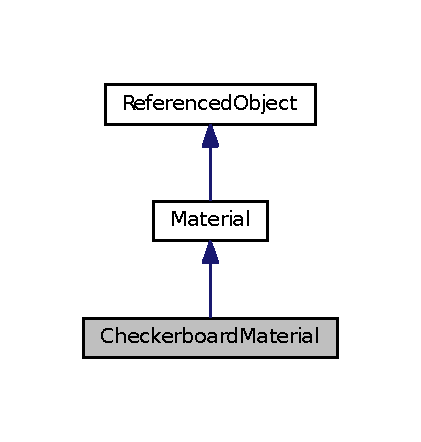
\includegraphics[width=202pt]{class_checkerboard_material__inherit__graph}
\end{center}
\end{figure}


Collaboration diagram for Checkerboard\+Material\+:
\nopagebreak
\begin{figure}[H]
\begin{center}
\leavevmode
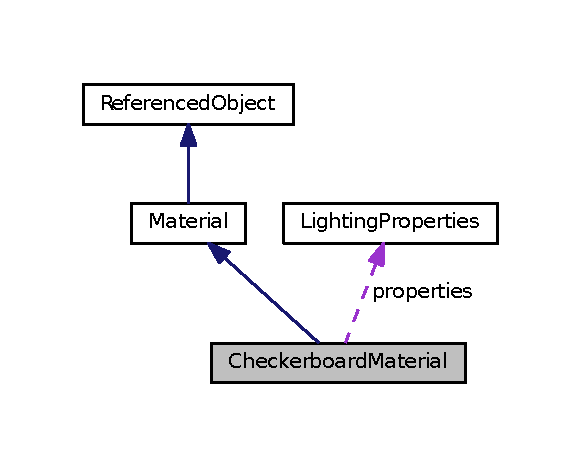
\includegraphics[width=279pt]{class_checkerboard_material__coll__graph}
\end{center}
\end{figure}
\subsection*{Public Member Functions}
\begin{DoxyCompactItemize}
\item 
{\bf Checkerboard\+Material} (double {\bf size}, {\bf Lighting\+Properties} $\ast$, {\bf Lighting\+Properties} $\ast$)
\item 
virtual void {\bf get\+Lighting\+Properties} (double point[3], {\bf Lighting\+Properties} $\ast$props, double normal[3])
\begin{DoxyCompactList}\small\item\em Returns the lighting properites at a certain point. \end{DoxyCompactList}\end{DoxyCompactItemize}
\subsection*{Private Attributes}
\begin{DoxyCompactItemize}
\item 
double {\bf size}
\item 
{\bf Lighting\+Properties} {\bf properties} [2]
\end{DoxyCompactItemize}


\subsection{Detailed Description}
A checkerboard pattern material. 

Requires checkerboard size and two sets of properties. 

Definition at line 75 of file material.\+h.



\subsection{Constructor \& Destructor Documentation}
\index{Checkerboard\+Material@{Checkerboard\+Material}!Checkerboard\+Material@{Checkerboard\+Material}}
\index{Checkerboard\+Material@{Checkerboard\+Material}!Checkerboard\+Material@{Checkerboard\+Material}}
\subsubsection[{Checkerboard\+Material}]{\setlength{\rightskip}{0pt plus 5cm}Checkerboard\+Material\+::\+Checkerboard\+Material (
\begin{DoxyParamCaption}
\item[{double}]{size, }
\item[{{\bf Lighting\+Properties} $\ast$}]{props\+A, }
\item[{{\bf Lighting\+Properties} $\ast$}]{props\+B}
\end{DoxyParamCaption}
)}\label{class_checkerboard_material_ae8ae0357838edb4f4ae27da273b7819f}


Definition at line 35 of file material.\+cc.



References properties, and size.



\subsection{Member Function Documentation}
\index{Checkerboard\+Material@{Checkerboard\+Material}!get\+Lighting\+Properties@{get\+Lighting\+Properties}}
\index{get\+Lighting\+Properties@{get\+Lighting\+Properties}!Checkerboard\+Material@{Checkerboard\+Material}}
\subsubsection[{get\+Lighting\+Properties}]{\setlength{\rightskip}{0pt plus 5cm}void Checkerboard\+Material\+::get\+Lighting\+Properties (
\begin{DoxyParamCaption}
\item[{double}]{point[3], }
\item[{{\bf Lighting\+Properties} $\ast$}]{props, }
\item[{double}]{normal[3]}
\end{DoxyParamCaption}
)\hspace{0.3cm}{\ttfamily [virtual]}}\label{class_checkerboard_material_a1fd16339705d7653381e72ee3d188613}


Returns the lighting properites at a certain point. 

Is also given the current normal at that point, and can modify it. 

Implements {\bf Material} \doxyref{}{p.}{class_material_ab61e7df6a740ad2ad3a82700005982bd}.



Definition at line 42 of file material.\+cc.



References properties, and size.



\subsection{Member Data Documentation}
\index{Checkerboard\+Material@{Checkerboard\+Material}!properties@{properties}}
\index{properties@{properties}!Checkerboard\+Material@{Checkerboard\+Material}}
\subsubsection[{properties}]{\setlength{\rightskip}{0pt plus 5cm}{\bf Lighting\+Properties} Checkerboard\+Material\+::properties[2]\hspace{0.3cm}{\ttfamily [private]}}\label{class_checkerboard_material_a02fdbb9c4d5aeca8e3f00d3bf4919d48}


Definition at line 82 of file material.\+h.



Referenced by Checkerboard\+Material(), and get\+Lighting\+Properties().

\index{Checkerboard\+Material@{Checkerboard\+Material}!size@{size}}
\index{size@{size}!Checkerboard\+Material@{Checkerboard\+Material}}
\subsubsection[{size}]{\setlength{\rightskip}{0pt plus 5cm}double Checkerboard\+Material\+::size\hspace{0.3cm}{\ttfamily [private]}}\label{class_checkerboard_material_a956d7bc460529a215a868c0ab9a4f806}


Definition at line 81 of file material.\+h.



Referenced by Checkerboard\+Material(), and get\+Lighting\+Properties().



The documentation for this class was generated from the following files\+:\begin{DoxyCompactItemize}
\item 
{\bf material.\+h}\item 
{\bf material.\+cc}\end{DoxyCompactItemize}

\section{Intersection Class Reference}
\label{class_intersection}\index{Intersection@{Intersection}}


Creates new objects as the intersection of multiple child objects.  




{\ttfamily \#include $<$csg.\+h$>$}



Inheritance diagram for Intersection\+:
\nopagebreak
\begin{figure}[H]
\begin{center}
\leavevmode
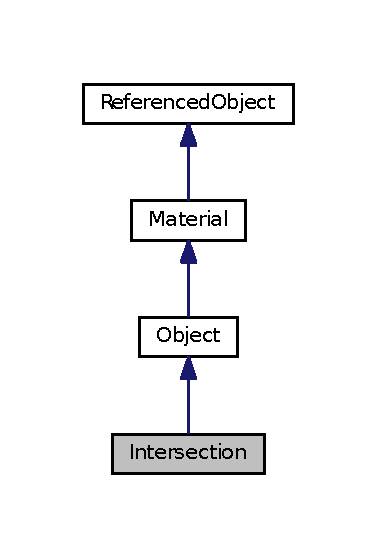
\includegraphics[width=181pt]{class_intersection__inherit__graph}
\end{center}
\end{figure}


Collaboration diagram for Intersection\+:
\nopagebreak
\begin{figure}[H]
\begin{center}
\leavevmode
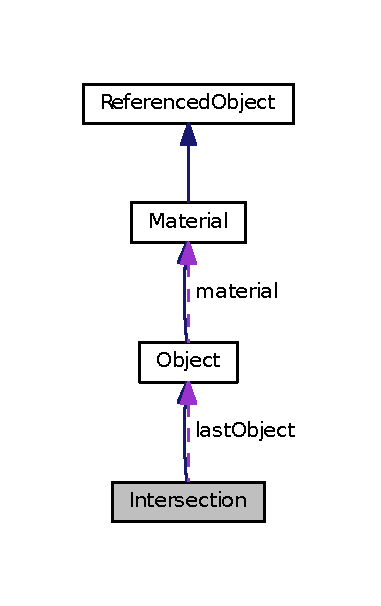
\includegraphics[width=183pt]{class_intersection__coll__graph}
\end{center}
\end{figure}
\subsection*{Public Member Functions}
\begin{DoxyCompactItemize}
\item 
{\bf Intersection} ()
\item 
{\bf $\sim$\+Intersection} ()
\item 
void {\bf add\+Object} ({\bf Object} $\ast$)
\item 
double {\bf line\+Test} (double origin[3], double direction[3], double max\+Distance)
\begin{DoxyCompactList}\small\item\em Must do the line intersection test and return the closest distance in which a ray originating in origin with given direction intersects the object -\/ if such a point exists closer than max\+Distance. \end{DoxyCompactList}\item 
void {\bf get\+Normal} (double point[3], double normal[3])
\begin{DoxyCompactList}\small\item\em Compute the normal of the object at the given point. \end{DoxyCompactList}\item 
bool {\bf is\+Inside} (double point[3])
\begin{DoxyCompactList}\small\item\em Tests if a point is inside the object or not. \end{DoxyCompactList}\item 
void {\bf get\+Lighting\+Properties} (double point[3], {\bf Lighting\+Properties} $\ast$props, double normal[3])
\begin{DoxyCompactList}\small\item\em Default material handling that queries the default material given for this object. \end{DoxyCompactList}\end{DoxyCompactItemize}
\subsection*{Private Attributes}
\begin{DoxyCompactItemize}
\item 
class std\+::set$<$ {\bf Object} $\ast$ $>$ $\ast$ {\bf objects}
\item 
{\bf Object} $\ast$ {\bf last\+Object} [{\bf M\+A\+X\+\_\+\+O\+M\+P\+\_\+\+T\+H\+R\+E\+A\+D\+S}]
\end{DoxyCompactItemize}
\subsection*{Additional Inherited Members}


\subsection{Detailed Description}
Creates new objects as the intersection of multiple child objects. 

This is one of the basic C\+S\+G building blocks of more complex geometry. In this current implementation it is done in a generic, but inefficeint manner. More efficient code can be made using harder restrictions on the contained child objects. 

Definition at line 38 of file csg.\+h.



\subsection{Constructor \& Destructor Documentation}
\index{Intersection@{Intersection}!Intersection@{Intersection}}
\index{Intersection@{Intersection}!Intersection@{Intersection}}
\subsubsection[{Intersection}]{\setlength{\rightskip}{0pt plus 5cm}Intersection\+::\+Intersection (
\begin{DoxyParamCaption}
{}
\end{DoxyParamCaption}
)}\label{class_intersection_a67497e3efe2793b23909052eeb82c4f3}


Definition at line 30 of file csg.\+cc.



References M\+A\+X\+\_\+\+O\+M\+P\+\_\+\+T\+H\+R\+E\+A\+D\+S.

\index{Intersection@{Intersection}!````~Intersection@{$\sim$\+Intersection}}
\index{````~Intersection@{$\sim$\+Intersection}!Intersection@{Intersection}}
\subsubsection[{$\sim$\+Intersection}]{\setlength{\rightskip}{0pt plus 5cm}Intersection\+::$\sim$\+Intersection (
\begin{DoxyParamCaption}
{}
\end{DoxyParamCaption}
)}\label{class_intersection_a064951a970ed8dd11081b2903ab62122}


Definition at line 34 of file csg.\+cc.



\subsection{Member Function Documentation}
\index{Intersection@{Intersection}!add\+Object@{add\+Object}}
\index{add\+Object@{add\+Object}!Intersection@{Intersection}}
\subsubsection[{add\+Object}]{\setlength{\rightskip}{0pt plus 5cm}void Intersection\+::add\+Object (
\begin{DoxyParamCaption}
\item[{{\bf Object} $\ast$}]{object}
\end{DoxyParamCaption}
)}\label{class_intersection_a62cc72188b282d2887f5979e7b5f5325}


Definition at line 42 of file csg.\+cc.



Referenced by main().

\index{Intersection@{Intersection}!get\+Lighting\+Properties@{get\+Lighting\+Properties}}
\index{get\+Lighting\+Properties@{get\+Lighting\+Properties}!Intersection@{Intersection}}
\subsubsection[{get\+Lighting\+Properties}]{\setlength{\rightskip}{0pt plus 5cm}void Intersection\+::get\+Lighting\+Properties (
\begin{DoxyParamCaption}
\item[{double}]{point[3], }
\item[{{\bf Lighting\+Properties} $\ast$}]{props, }
\item[{double}]{normal[3]}
\end{DoxyParamCaption}
)\hspace{0.3cm}{\ttfamily [virtual]}}\label{class_intersection_aeaf604c0cdbef2d4c2a0f2087287ead8}


Default material handling that queries the default material given for this object. 



Reimplemented from {\bf Object} \doxyref{}{p.}{class_object_a510171215bdf364cc0bf8f72336039b9}.



Definition at line 137 of file csg.\+cc.

\index{Intersection@{Intersection}!get\+Normal@{get\+Normal}}
\index{get\+Normal@{get\+Normal}!Intersection@{Intersection}}
\subsubsection[{get\+Normal}]{\setlength{\rightskip}{0pt plus 5cm}void Intersection\+::get\+Normal (
\begin{DoxyParamCaption}
\item[{double}]{point[3], }
\item[{double}]{normal[3]}
\end{DoxyParamCaption}
)\hspace{0.3cm}{\ttfamily [virtual]}}\label{class_intersection_aca5201537e1f12305142be681b0e0b47}


Compute the normal of the object at the given point. 

Result is not guaranteed to be of unit length. 

Implements {\bf Object} \doxyref{}{p.}{class_object_a22c15ace5725e2577dbb187265bd3201}.



Definition at line 114 of file csg.\+cc.

\index{Intersection@{Intersection}!is\+Inside@{is\+Inside}}
\index{is\+Inside@{is\+Inside}!Intersection@{Intersection}}
\subsubsection[{is\+Inside}]{\setlength{\rightskip}{0pt plus 5cm}bool Intersection\+::is\+Inside (
\begin{DoxyParamCaption}
\item[{double}]{point[3]}
\end{DoxyParamCaption}
)\hspace{0.3cm}{\ttfamily [virtual]}}\label{class_intersection_acbba7803bcd3928967fd675992a8ae96}


Tests if a point is inside the object or not. 



Implements {\bf Object} \doxyref{}{p.}{class_object_a652359286747bf237cb2d4d0a802bd18}.



Definition at line 125 of file csg.\+cc.

\index{Intersection@{Intersection}!line\+Test@{line\+Test}}
\index{line\+Test@{line\+Test}!Intersection@{Intersection}}
\subsubsection[{line\+Test}]{\setlength{\rightskip}{0pt plus 5cm}double Intersection\+::line\+Test (
\begin{DoxyParamCaption}
\item[{double}]{origin[3], }
\item[{double}]{direction[3], }
\item[{double}]{max\+Distance}
\end{DoxyParamCaption}
)\hspace{0.3cm}{\ttfamily [virtual]}}\label{class_intersection_acadaeb4e35a52f4d1ff80769586921ff}


Must do the line intersection test and return the closest distance in which a ray originating in origin with given direction intersects the object -\/ if such a point exists closer than max\+Distance. 

Returns distance M\+A\+X\+\_\+\+D\+I\+S\+T\+A\+N\+C\+E if no such intersection exists.

Direction is not neccessarily a vector of unit length, and distances are measured in multiples of this vector. 

Implements {\bf Object} \doxyref{}{p.}{class_object_a1bfd7ffbccda28c67d8a537393113a7e}.



Definition at line 47 of file csg.\+cc.



References assign(), debug\+Indentation, debug\+This\+Pixel, M\+A\+X\+\_\+\+D\+I\+S\+T\+A\+N\+C\+E, and print\+Debug\+Indentation().



\subsection{Member Data Documentation}
\index{Intersection@{Intersection}!last\+Object@{last\+Object}}
\index{last\+Object@{last\+Object}!Intersection@{Intersection}}
\subsubsection[{last\+Object}]{\setlength{\rightskip}{0pt plus 5cm}{\bf Object}$\ast$ Intersection\+::last\+Object[{\bf M\+A\+X\+\_\+\+O\+M\+P\+\_\+\+T\+H\+R\+E\+A\+D\+S}]\hspace{0.3cm}{\ttfamily [private]}}\label{class_intersection_a4bb95b11d0d394e87971b20b1cb12f45}


Definition at line 53 of file csg.\+h.

\index{Intersection@{Intersection}!objects@{objects}}
\index{objects@{objects}!Intersection@{Intersection}}
\subsubsection[{objects}]{\setlength{\rightskip}{0pt plus 5cm}class std\+::set$<$ {\bf Object} $\ast$ $>$$\ast$ Intersection\+::objects\hspace{0.3cm}{\ttfamily [private]}}\label{class_intersection_aa44bbc9287dbeaf174128bdbbba0ca71}


Definition at line 51 of file csg.\+h.



The documentation for this class was generated from the following files\+:\begin{DoxyCompactItemize}
\item 
{\bf csg.\+h}\item 
{\bf csg.\+cc}\end{DoxyCompactItemize}

\section{Inverse Class Reference}
\label{class_inverse}\index{Inverse@{Inverse}}


Creates the inverse of an object by negating the \doxyref{Object\+::is\+Inside}{p.}{class_object_a652359286747bf237cb2d4d0a802bd18} and Object\+::\+Get\+Normal functions.  




{\ttfamily \#include $<$csg.\+h$>$}



Inheritance diagram for Inverse\+:
\nopagebreak
\begin{figure}[H]
\begin{center}
\leavevmode
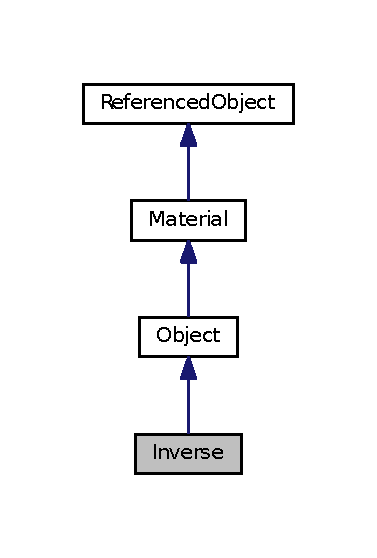
\includegraphics[width=181pt]{class_inverse__inherit__graph}
\end{center}
\end{figure}


Collaboration diagram for Inverse\+:
\nopagebreak
\begin{figure}[H]
\begin{center}
\leavevmode
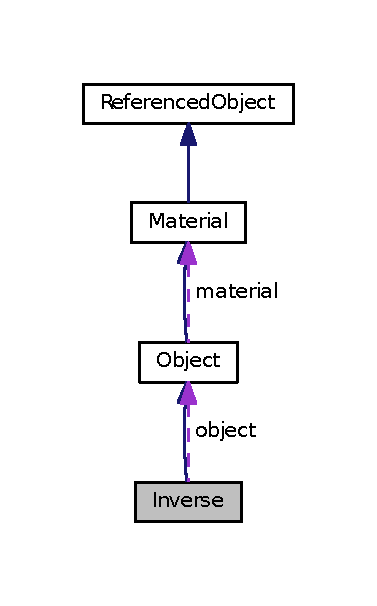
\includegraphics[width=181pt]{class_inverse__coll__graph}
\end{center}
\end{figure}
\subsection*{Public Member Functions}
\begin{DoxyCompactItemize}
\item 
{\bf Inverse} ({\bf Object} $\ast$)
\item 
{\bf $\sim$\+Inverse} ()
\item 
double {\bf line\+Test} (double origin[3], double direction[3], double max\+Distance)
\begin{DoxyCompactList}\small\item\em Must do the line intersection test and return the closest distance in which a ray originating in origin with given direction intersects the object -\/ if such a point exists closer than max\+Distance. \end{DoxyCompactList}\item 
void {\bf get\+Normal} (double point[3], double normal[3])
\begin{DoxyCompactList}\small\item\em Compute the normal of the object at the given point. \end{DoxyCompactList}\item 
bool {\bf is\+Inside} (double point[3])
\begin{DoxyCompactList}\small\item\em Tests if a point is inside the object or not. \end{DoxyCompactList}\item 
void {\bf get\+Lighting\+Properties} (double point[3], {\bf Lighting\+Properties} $\ast$props, double normal[3])
\begin{DoxyCompactList}\small\item\em Default material handling that queries the default material given for this object. \end{DoxyCompactList}\end{DoxyCompactItemize}
\subsection*{Private Attributes}
\begin{DoxyCompactItemize}
\item 
{\bf Object} $\ast$ {\bf object}
\end{DoxyCompactItemize}
\subsection*{Additional Inherited Members}


\subsection{Detailed Description}
Creates the inverse of an object by negating the \doxyref{Object\+::is\+Inside}{p.}{class_object_a652359286747bf237cb2d4d0a802bd18} and Object\+::\+Get\+Normal functions. 



Definition at line 58 of file csg.\+h.



\subsection{Constructor \& Destructor Documentation}
\index{Inverse@{Inverse}!Inverse@{Inverse}}
\index{Inverse@{Inverse}!Inverse@{Inverse}}
\subsubsection[{Inverse}]{\setlength{\rightskip}{0pt plus 5cm}Inverse\+::\+Inverse (
\begin{DoxyParamCaption}
\item[{{\bf Object} $\ast$}]{o}
\end{DoxyParamCaption}
)}\label{class_inverse_ab465fd57124caf679827ec3dddabe2ea}


Definition at line 148 of file csg.\+cc.



References Referenced\+Object\+::reference().

\index{Inverse@{Inverse}!````~Inverse@{$\sim$\+Inverse}}
\index{````~Inverse@{$\sim$\+Inverse}!Inverse@{Inverse}}
\subsubsection[{$\sim$\+Inverse}]{\setlength{\rightskip}{0pt plus 5cm}Inverse\+::$\sim$\+Inverse (
\begin{DoxyParamCaption}
{}
\end{DoxyParamCaption}
)}\label{class_inverse_a21add8a55de3e5c898701e0a22a12cc1}


Definition at line 149 of file csg.\+cc.



\subsection{Member Function Documentation}
\index{Inverse@{Inverse}!get\+Lighting\+Properties@{get\+Lighting\+Properties}}
\index{get\+Lighting\+Properties@{get\+Lighting\+Properties}!Inverse@{Inverse}}
\subsubsection[{get\+Lighting\+Properties}]{\setlength{\rightskip}{0pt plus 5cm}void Inverse\+::get\+Lighting\+Properties (
\begin{DoxyParamCaption}
\item[{double}]{point[3], }
\item[{{\bf Lighting\+Properties} $\ast$}]{props, }
\item[{double}]{normal[3]}
\end{DoxyParamCaption}
)\hspace{0.3cm}{\ttfamily [virtual]}}\label{class_inverse_abedf66c2607143f237f913187ecfdc40}


Default material handling that queries the default material given for this object. 



Reimplemented from {\bf Object} \doxyref{}{p.}{class_object_a510171215bdf364cc0bf8f72336039b9}.



Definition at line 161 of file csg.\+cc.

\index{Inverse@{Inverse}!get\+Normal@{get\+Normal}}
\index{get\+Normal@{get\+Normal}!Inverse@{Inverse}}
\subsubsection[{get\+Normal}]{\setlength{\rightskip}{0pt plus 5cm}void Inverse\+::get\+Normal (
\begin{DoxyParamCaption}
\item[{double}]{point[3], }
\item[{double}]{normal[3]}
\end{DoxyParamCaption}
)\hspace{0.3cm}{\ttfamily [virtual]}}\label{class_inverse_aead295a76d1bd7d8478fc0e32710c84f}


Compute the normal of the object at the given point. 

Result is not guaranteed to be of unit length. 

Implements {\bf Object} \doxyref{}{p.}{class_object_a22c15ace5725e2577dbb187265bd3201}.



Definition at line 153 of file csg.\+cc.

\index{Inverse@{Inverse}!is\+Inside@{is\+Inside}}
\index{is\+Inside@{is\+Inside}!Inverse@{Inverse}}
\subsubsection[{is\+Inside}]{\setlength{\rightskip}{0pt plus 5cm}bool Inverse\+::is\+Inside (
\begin{DoxyParamCaption}
\item[{double}]{point[3]}
\end{DoxyParamCaption}
)\hspace{0.3cm}{\ttfamily [virtual]}}\label{class_inverse_af3747e94047e18d4eff0fc61a92bf915}


Tests if a point is inside the object or not. 



Implements {\bf Object} \doxyref{}{p.}{class_object_a652359286747bf237cb2d4d0a802bd18}.



Definition at line 158 of file csg.\+cc.

\index{Inverse@{Inverse}!line\+Test@{line\+Test}}
\index{line\+Test@{line\+Test}!Inverse@{Inverse}}
\subsubsection[{line\+Test}]{\setlength{\rightskip}{0pt plus 5cm}double Inverse\+::line\+Test (
\begin{DoxyParamCaption}
\item[{double}]{origin[3], }
\item[{double}]{direction[3], }
\item[{double}]{max\+Distance}
\end{DoxyParamCaption}
)\hspace{0.3cm}{\ttfamily [virtual]}}\label{class_inverse_a7cd665a12ccf90142526965dfe416d1f}


Must do the line intersection test and return the closest distance in which a ray originating in origin with given direction intersects the object -\/ if such a point exists closer than max\+Distance. 

Returns distance M\+A\+X\+\_\+\+D\+I\+S\+T\+A\+N\+C\+E if no such intersection exists.

Direction is not neccessarily a vector of unit length, and distances are measured in multiples of this vector. 

Implements {\bf Object} \doxyref{}{p.}{class_object_a1bfd7ffbccda28c67d8a537393113a7e}.



Definition at line 150 of file csg.\+cc.



\subsection{Member Data Documentation}
\index{Inverse@{Inverse}!object@{object}}
\index{object@{object}!Inverse@{Inverse}}
\subsubsection[{object}]{\setlength{\rightskip}{0pt plus 5cm}{\bf Object}$\ast$ Inverse\+::object\hspace{0.3cm}{\ttfamily [private]}}\label{class_inverse_a744f471528f6830a87d04d3e88fd38c1}


Definition at line 69 of file csg.\+h.



The documentation for this class was generated from the following files\+:\begin{DoxyCompactItemize}
\item 
{\bf csg.\+h}\item 
{\bf csg.\+cc}\end{DoxyCompactItemize}

\section{Light Class Reference}
\label{class_light}\index{Light@{Light}}


Represents a simple direct point light in the scene.  




{\ttfamily \#include $<$light.\+h$>$}



Inheritance diagram for Light\+:
\nopagebreak
\begin{figure}[H]
\begin{center}
\leavevmode
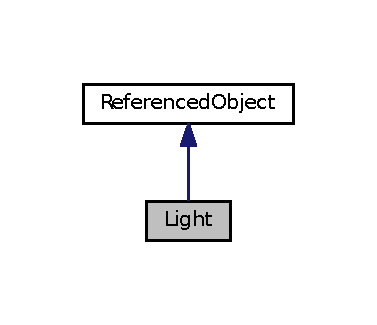
\includegraphics[width=181pt]{class_light__inherit__graph}
\end{center}
\end{figure}


Collaboration diagram for Light\+:
\nopagebreak
\begin{figure}[H]
\begin{center}
\leavevmode
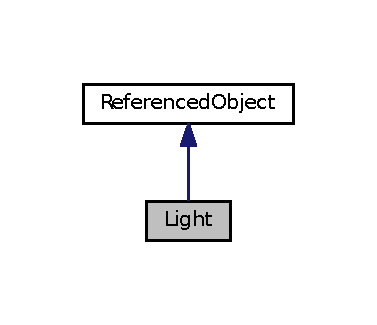
\includegraphics[width=181pt]{class_light__coll__graph}
\end{center}
\end{figure}
\subsection*{Public Member Functions}
\begin{DoxyCompactItemize}
\item 
{\bf Light} (double {\bf position}[3], double {\bf colour}[3])
\end{DoxyCompactItemize}
\subsection*{Private Attributes}
\begin{DoxyCompactItemize}
\item 
double {\bf position} [3]
\item 
double {\bf colour} [3]
\end{DoxyCompactItemize}
\subsection*{Friends}
\begin{DoxyCompactItemize}
\item 
class {\bf Raytracer}
\end{DoxyCompactItemize}


\subsection{Detailed Description}
Represents a simple direct point light in the scene. 

Must be added to the raytracer using the raytracer\+::add\+Light function. 

Definition at line 34 of file light.\+h.



\subsection{Constructor \& Destructor Documentation}
\index{Light@{Light}!Light@{Light}}
\index{Light@{Light}!Light@{Light}}
\subsubsection[{Light}]{\setlength{\rightskip}{0pt plus 5cm}Light\+::\+Light (
\begin{DoxyParamCaption}
\item[{double}]{position[3], }
\item[{double}]{colour[3]}
\end{DoxyParamCaption}
)}\label{class_light_abebfe14faccfd16ddb4b6548d5898857}


Definition at line 27 of file light.\+cc.



References assign(), colour, and position.



\subsection{Friends And Related Function Documentation}
\index{Light@{Light}!Raytracer@{Raytracer}}
\index{Raytracer@{Raytracer}!Light@{Light}}
\subsubsection[{Raytracer}]{\setlength{\rightskip}{0pt plus 5cm}friend class {\bf Raytracer}\hspace{0.3cm}{\ttfamily [friend]}}\label{class_light_abdcaeaebdde8832b52218293829319d1}


Definition at line 41 of file light.\+h.



\subsection{Member Data Documentation}
\index{Light@{Light}!colour@{colour}}
\index{colour@{colour}!Light@{Light}}
\subsubsection[{colour}]{\setlength{\rightskip}{0pt plus 5cm}double Light\+::colour[3]\hspace{0.3cm}{\ttfamily [private]}}\label{class_light_afa2b33995ca8745650d9dbc98dbb8710}


Definition at line 39 of file light.\+h.



Referenced by Light(), and Raytracer\+::raytrace().

\index{Light@{Light}!position@{position}}
\index{position@{position}!Light@{Light}}
\subsubsection[{position}]{\setlength{\rightskip}{0pt plus 5cm}double Light\+::position[3]\hspace{0.3cm}{\ttfamily [private]}}\label{class_light_a6fcf74c8199df0c6fdfb10afe0c0fac1}


Definition at line 38 of file light.\+h.



Referenced by Light(), and Raytracer\+::raytrace().



The documentation for this class was generated from the following files\+:\begin{DoxyCompactItemize}
\item 
{\bf light.\+h}\item 
{\bf light.\+cc}\end{DoxyCompactItemize}

\section{Lighting\+Properties Class Reference}
\label{class_lighting_properties}\index{Lighting\+Properties@{Lighting\+Properties}}


Stores lighting properties used for Phong lighting, reflections and transparancy.  




{\ttfamily \#include $<$material.\+h$>$}

\subsection*{Public Attributes}
\begin{DoxyCompactItemize}
\item 
double {\bf ambient} [3]
\item 
double {\bf diffuse} [3]
\item 
double {\bf specular} [3]
\item 
double {\bf shininess}
\item 
double {\bf reflection} [3]
\end{DoxyCompactItemize}


\subsection{Detailed Description}
Stores lighting properties used for Phong lighting, reflections and transparancy. 

Must be given by any custom defined material on a per pixel basis. 

Definition at line 37 of file material.\+h.



\subsection{Member Data Documentation}
\index{Lighting\+Properties@{Lighting\+Properties}!ambient@{ambient}}
\index{ambient@{ambient}!Lighting\+Properties@{Lighting\+Properties}}
\subsubsection[{ambient}]{\setlength{\rightskip}{0pt plus 5cm}double Lighting\+Properties\+::ambient[3]}\label{class_lighting_properties_a10acb0d655b119de855389ec9840ca8e}


Definition at line 39 of file material.\+h.



Referenced by Noise\+Material\+::get\+Lighting\+Properties(), Material\+Map\+::get\+Lighting\+Properties(), and Raytracer\+::raytrace().

\index{Lighting\+Properties@{Lighting\+Properties}!diffuse@{diffuse}}
\index{diffuse@{diffuse}!Lighting\+Properties@{Lighting\+Properties}}
\subsubsection[{diffuse}]{\setlength{\rightskip}{0pt plus 5cm}double Lighting\+Properties\+::diffuse[3]}\label{class_lighting_properties_a2929421503c5030cb19a5f8eefabbfdd}


Definition at line 40 of file material.\+h.



Referenced by Noise\+Material\+::get\+Lighting\+Properties(), Material\+Map\+::get\+Lighting\+Properties(), and Raytracer\+::raytrace().

\index{Lighting\+Properties@{Lighting\+Properties}!reflection@{reflection}}
\index{reflection@{reflection}!Lighting\+Properties@{Lighting\+Properties}}
\subsubsection[{reflection}]{\setlength{\rightskip}{0pt plus 5cm}double Lighting\+Properties\+::reflection[3]}\label{class_lighting_properties_a39dea5f8dd780e1ab17261ab3503795d}


Definition at line 42 of file material.\+h.



Referenced by Noise\+Material\+::get\+Lighting\+Properties(), Material\+Map\+::get\+Lighting\+Properties(), and Raytracer\+::raytrace().

\index{Lighting\+Properties@{Lighting\+Properties}!shininess@{shininess}}
\index{shininess@{shininess}!Lighting\+Properties@{Lighting\+Properties}}
\subsubsection[{shininess}]{\setlength{\rightskip}{0pt plus 5cm}double Lighting\+Properties\+::shininess}\label{class_lighting_properties_a213c42ef1df28e24a0b737ea6a5907f4}


Definition at line 41 of file material.\+h.



Referenced by Noise\+Material\+::get\+Lighting\+Properties(), Material\+Map\+::get\+Lighting\+Properties(), and Raytracer\+::raytrace().

\index{Lighting\+Properties@{Lighting\+Properties}!specular@{specular}}
\index{specular@{specular}!Lighting\+Properties@{Lighting\+Properties}}
\subsubsection[{specular}]{\setlength{\rightskip}{0pt plus 5cm}double Lighting\+Properties\+::specular[3]}\label{class_lighting_properties_a51c284c37c2b0ce9eb430b2091254eb8}


Definition at line 41 of file material.\+h.



Referenced by Noise\+Material\+::get\+Lighting\+Properties(), Material\+Map\+::get\+Lighting\+Properties(), and Raytracer\+::raytrace().



The documentation for this class was generated from the following file\+:\begin{DoxyCompactItemize}
\item 
{\bf material.\+h}\end{DoxyCompactItemize}

\section{Material Class Reference}
\label{class_material}\index{Material@{Material}}


Abstract base class for all materials.  




{\ttfamily \#include $<$material.\+h$>$}



Inheritance diagram for Material\+:
\nopagebreak
\begin{figure}[H]
\begin{center}
\leavevmode
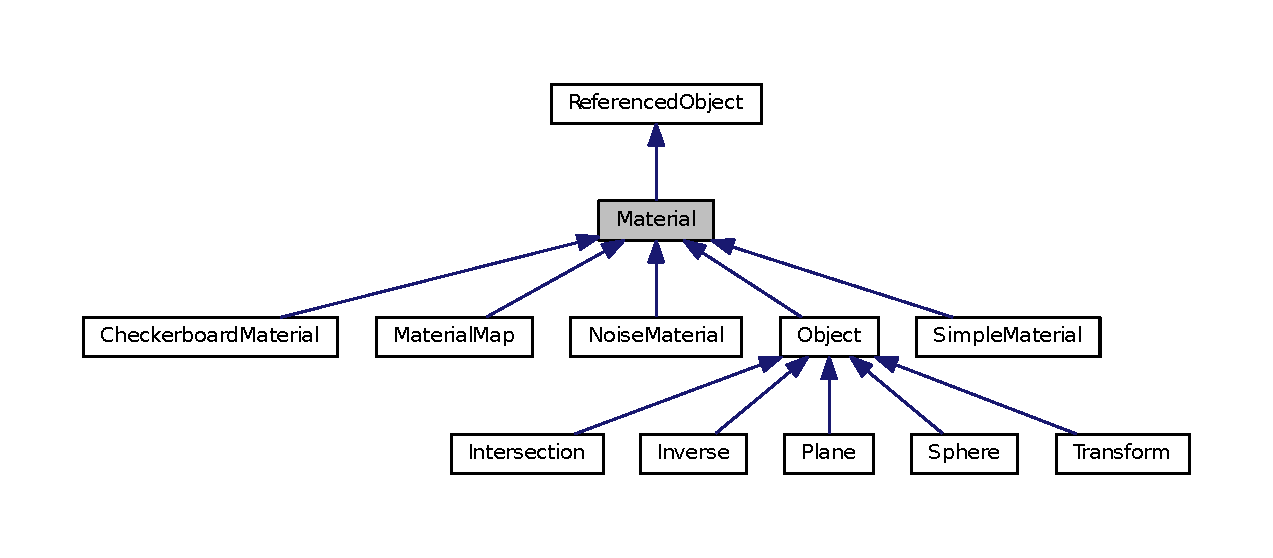
\includegraphics[width=350pt]{class_material__inherit__graph}
\end{center}
\end{figure}


Collaboration diagram for Material\+:
\nopagebreak
\begin{figure}[H]
\begin{center}
\leavevmode
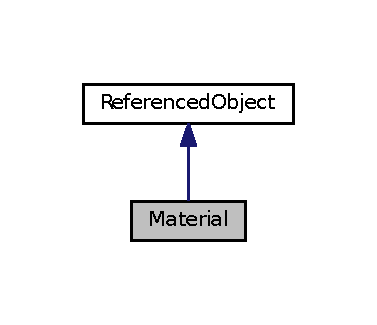
\includegraphics[width=181pt]{class_material__coll__graph}
\end{center}
\end{figure}
\subsection*{Public Member Functions}
\begin{DoxyCompactItemize}
\item 
{\bf Material} ()
\item 
virtual void {\bf get\+Lighting\+Properties} (double point[3], {\bf Lighting\+Properties} $\ast$props, double normal[3])=0
\begin{DoxyCompactList}\small\item\em Returns the lighting properites at a certain point. \end{DoxyCompactList}\end{DoxyCompactItemize}


\subsection{Detailed Description}
Abstract base class for all materials. 

These objects are used to compute the lighting properties for any specific point in the scene using the virtual function \doxyref{Material\+::get\+Lighting\+Properties()}{p.}{class_material_ab61e7df6a740ad2ad3a82700005982bd}. 

Definition at line 51 of file material.\+h.



\subsection{Constructor \& Destructor Documentation}
\index{Material@{Material}!Material@{Material}}
\index{Material@{Material}!Material@{Material}}
\subsubsection[{Material}]{\setlength{\rightskip}{0pt plus 5cm}Material\+::\+Material (
\begin{DoxyParamCaption}
{}
\end{DoxyParamCaption}
)}\label{class_material_a137e987401b63eb7c6c27c3e38bc74b5}


Definition at line 29 of file material.\+cc.



\subsection{Member Function Documentation}
\index{Material@{Material}!get\+Lighting\+Properties@{get\+Lighting\+Properties}}
\index{get\+Lighting\+Properties@{get\+Lighting\+Properties}!Material@{Material}}
\subsubsection[{get\+Lighting\+Properties}]{\setlength{\rightskip}{0pt plus 5cm}virtual void Material\+::get\+Lighting\+Properties (
\begin{DoxyParamCaption}
\item[{double}]{point[3], }
\item[{{\bf Lighting\+Properties} $\ast$}]{props, }
\item[{double}]{normal[3]}
\end{DoxyParamCaption}
)\hspace{0.3cm}{\ttfamily [pure virtual]}}\label{class_material_ab61e7df6a740ad2ad3a82700005982bd}


Returns the lighting properites at a certain point. 

Is also given the current normal at that point, and can modify it. 

Implemented in {\bf Material\+Map} \doxyref{}{p.}{class_material_map_abd631c6e7b36737bcaadffbf47ca60aa}, {\bf Noise\+Material} \doxyref{}{p.}{class_noise_material_a07c6bb884031fea88df86e8d9fd85bec}, {\bf Checkerboard\+Material} \doxyref{}{p.}{class_checkerboard_material_a1fd16339705d7653381e72ee3d188613}, {\bf Inverse} \doxyref{}{p.}{class_inverse_abedf66c2607143f237f913187ecfdc40}, {\bf Simple\+Material} \doxyref{}{p.}{class_simple_material_a23e6ee14c9b9f1bd369023472f676168}, {\bf Object} \doxyref{}{p.}{class_object_a510171215bdf364cc0bf8f72336039b9}, {\bf Transform} \doxyref{}{p.}{class_transform_a6759fe52b87d9113c48c0414824ac067}, and {\bf Intersection} \doxyref{}{p.}{class_intersection_aeaf604c0cdbef2d4c2a0f2087287ead8}.



Referenced by Transform\+::get\+Lighting\+Properties(), and Object\+::get\+Lighting\+Properties().



The documentation for this class was generated from the following files\+:\begin{DoxyCompactItemize}
\item 
{\bf material.\+h}\item 
{\bf material.\+cc}\end{DoxyCompactItemize}

\section{Material\+Map Class Reference}
\label{class_material_map}\index{Material\+Map@{Material\+Map}}


Generic function mapped material.  




{\ttfamily \#include $<$material.\+h$>$}



Inheritance diagram for Material\+Map\+:
\nopagebreak
\begin{figure}[H]
\begin{center}
\leavevmode
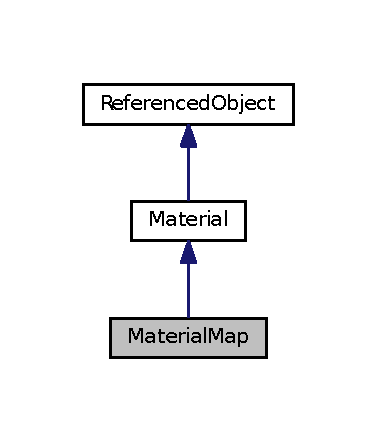
\includegraphics[width=181pt]{class_material_map__inherit__graph}
\end{center}
\end{figure}


Collaboration diagram for Material\+Map\+:
\nopagebreak
\begin{figure}[H]
\begin{center}
\leavevmode
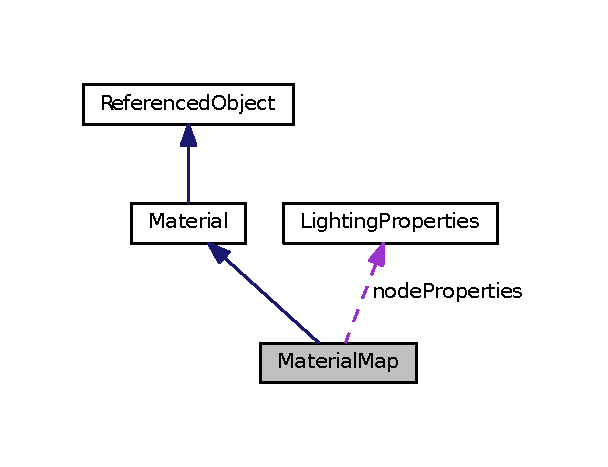
\includegraphics[width=292pt]{class_material_map__coll__graph}
\end{center}
\end{figure}
\subsection*{Public Types}
\begin{DoxyCompactItemize}
\item 
enum {\bf Function} \{ {\bf Noise}
 \}
\end{DoxyCompactItemize}
\subsection*{Public Member Functions}
\begin{DoxyCompactItemize}
\item 
{\bf Material\+Map} ({\bf Function} fun)
\item 
void {\bf add} (double node\+Position, {\bf Lighting\+Properties} $\ast${\bf node\+Properties})
\item 
virtual void {\bf get\+Lighting\+Properties} (double point[3], {\bf Lighting\+Properties} $\ast$props, double normal[3])
\begin{DoxyCompactList}\small\item\em Returns the lighting properites at a certain point. \end{DoxyCompactList}\end{DoxyCompactItemize}
\subsection*{Private Attributes}
\begin{DoxyCompactItemize}
\item 
{\bf Function} {\bf function}
\item 
double {\bf node\+Positions} [{\bf M\+A\+X\+\_\+\+M\+A\+T\+E\+R\+I\+A\+L\+\_\+\+M\+A\+P\+\_\+\+N\+O\+D\+E\+S}]
\item 
{\bf Lighting\+Properties} {\bf node\+Properties} [{\bf M\+A\+X\+\_\+\+M\+A\+T\+E\+R\+I\+A\+L\+\_\+\+M\+A\+P\+\_\+\+N\+O\+D\+E\+S}]
\item 
int {\bf n\+Nodes}
\end{DoxyCompactItemize}


\subsection{Detailed Description}
Generic function mapped material. 

Interpolatates between multiple lighting properties depending on a given function. To use, instantiate with a given function and add all \doxyref{Lighting\+Properties}{p.}{class_lighting_properties} nodes that you want to interpolate between. Each node should be given a function value for which it will contribute 100\% to the resulting material property. 

Definition at line 101 of file material.\+h.



\subsection{Member Enumeration Documentation}
\index{Material\+Map@{Material\+Map}!Function@{Function}}
\index{Function@{Function}!Material\+Map@{Material\+Map}}
\subsubsection[{Function}]{\setlength{\rightskip}{0pt plus 5cm}enum {\bf Material\+Map\+::\+Function}}\label{class_material_map_a8421b6a814d23308f82ae8aa65210d2c}
\begin{Desc}
\item[Enumerator]\par
\begin{description}
\index{Noise@{Noise}!Material\+Map@{Material\+Map}}\index{Material\+Map@{Material\+Map}!Noise@{Noise}}\item[{\em 
Noise\label{class_material_map_a8421b6a814d23308f82ae8aa65210d2ca7335266b92cfbd695f89bdf112475089}
}]\end{description}
\end{Desc}


Definition at line 103 of file material.\+h.



\subsection{Constructor \& Destructor Documentation}
\index{Material\+Map@{Material\+Map}!Material\+Map@{Material\+Map}}
\index{Material\+Map@{Material\+Map}!Material\+Map@{Material\+Map}}
\subsubsection[{Material\+Map}]{\setlength{\rightskip}{0pt plus 5cm}Material\+Map\+::\+Material\+Map (
\begin{DoxyParamCaption}
\item[{{\bf Function}}]{fun}
\end{DoxyParamCaption}
)}\label{class_material_map_a5edcadc83453646f73c0b9214ff67937}


Definition at line 70 of file material.\+cc.



References n\+Nodes.



\subsection{Member Function Documentation}
\index{Material\+Map@{Material\+Map}!add@{add}}
\index{add@{add}!Material\+Map@{Material\+Map}}
\subsubsection[{add}]{\setlength{\rightskip}{0pt plus 5cm}void Material\+Map\+::add (
\begin{DoxyParamCaption}
\item[{double}]{node\+Position, }
\item[{{\bf Lighting\+Properties} $\ast$}]{node\+Properties}
\end{DoxyParamCaption}
)}\label{class_material_map_ac0b6b46d1364415e48867ffd550a0cad}


Definition at line 76 of file material.\+cc.



References n\+Nodes, node\+Positions, and node\+Properties.



Referenced by main().

\index{Material\+Map@{Material\+Map}!get\+Lighting\+Properties@{get\+Lighting\+Properties}}
\index{get\+Lighting\+Properties@{get\+Lighting\+Properties}!Material\+Map@{Material\+Map}}
\subsubsection[{get\+Lighting\+Properties}]{\setlength{\rightskip}{0pt plus 5cm}void Material\+Map\+::get\+Lighting\+Properties (
\begin{DoxyParamCaption}
\item[{double}]{point[3], }
\item[{{\bf Lighting\+Properties} $\ast$}]{props, }
\item[{double}]{normal[3]}
\end{DoxyParamCaption}
)\hspace{0.3cm}{\ttfamily [virtual]}}\label{class_material_map_abd631c6e7b36737bcaadffbf47ca60aa}


Returns the lighting properites at a certain point. 

Is also given the current normal at that point, and can modify it. 

Implements {\bf Material} \doxyref{}{p.}{class_material_ab61e7df6a740ad2ad3a82700005982bd}.



Definition at line 93 of file material.\+cc.



References Lighting\+Properties\+::ambient, Lighting\+Properties\+::diffuse, n\+Nodes, node\+Positions, node\+Properties, noise(), Lighting\+Properties\+::reflection, Lighting\+Properties\+::shininess, Lighting\+Properties\+::specular, and zero().



\subsection{Member Data Documentation}
\index{Material\+Map@{Material\+Map}!function@{function}}
\index{function@{function}!Material\+Map@{Material\+Map}}
\subsubsection[{function}]{\setlength{\rightskip}{0pt plus 5cm}{\bf Function} Material\+Map\+::function\hspace{0.3cm}{\ttfamily [private]}}\label{class_material_map_a6e67e48f7ec5ba054d0223bd63914880}


Definition at line 108 of file material.\+h.

\index{Material\+Map@{Material\+Map}!n\+Nodes@{n\+Nodes}}
\index{n\+Nodes@{n\+Nodes}!Material\+Map@{Material\+Map}}
\subsubsection[{n\+Nodes}]{\setlength{\rightskip}{0pt plus 5cm}int Material\+Map\+::n\+Nodes\hspace{0.3cm}{\ttfamily [private]}}\label{class_material_map_ad4bd914574ead4cc4bd5519bc595bfc2}


Definition at line 111 of file material.\+h.



Referenced by add(), get\+Lighting\+Properties(), and Material\+Map().

\index{Material\+Map@{Material\+Map}!node\+Positions@{node\+Positions}}
\index{node\+Positions@{node\+Positions}!Material\+Map@{Material\+Map}}
\subsubsection[{node\+Positions}]{\setlength{\rightskip}{0pt plus 5cm}double Material\+Map\+::node\+Positions[{\bf M\+A\+X\+\_\+\+M\+A\+T\+E\+R\+I\+A\+L\+\_\+\+M\+A\+P\+\_\+\+N\+O\+D\+E\+S}]\hspace{0.3cm}{\ttfamily [private]}}\label{class_material_map_aa6fb5977287c2b9dddb56b49db4c55b6}


Definition at line 109 of file material.\+h.



Referenced by add(), and get\+Lighting\+Properties().

\index{Material\+Map@{Material\+Map}!node\+Properties@{node\+Properties}}
\index{node\+Properties@{node\+Properties}!Material\+Map@{Material\+Map}}
\subsubsection[{node\+Properties}]{\setlength{\rightskip}{0pt plus 5cm}{\bf Lighting\+Properties} Material\+Map\+::node\+Properties[{\bf M\+A\+X\+\_\+\+M\+A\+T\+E\+R\+I\+A\+L\+\_\+\+M\+A\+P\+\_\+\+N\+O\+D\+E\+S}]\hspace{0.3cm}{\ttfamily [private]}}\label{class_material_map_ad549e9c01455af303728a60d85b3286f}


Definition at line 110 of file material.\+h.



Referenced by add(), and get\+Lighting\+Properties().



The documentation for this class was generated from the following files\+:\begin{DoxyCompactItemize}
\item 
{\bf material.\+h}\item 
{\bf material.\+cc}\end{DoxyCompactItemize}

\section{Noise\+Material Class Reference}
\label{class_noise_material}\index{Noise\+Material@{Noise\+Material}}


Creates gray noise all over the object.  




{\ttfamily \#include $<$material.\+h$>$}



Inheritance diagram for Noise\+Material\+:
\nopagebreak
\begin{figure}[H]
\begin{center}
\leavevmode
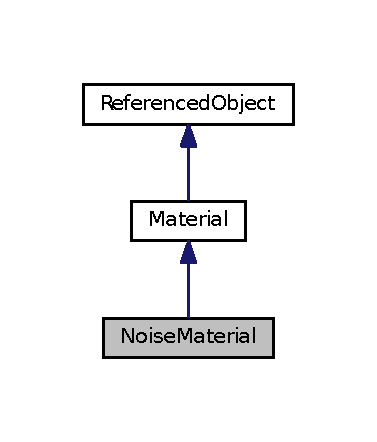
\includegraphics[width=181pt]{class_noise_material__inherit__graph}
\end{center}
\end{figure}


Collaboration diagram for Noise\+Material\+:
\nopagebreak
\begin{figure}[H]
\begin{center}
\leavevmode
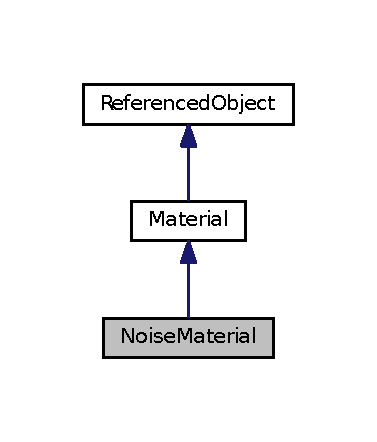
\includegraphics[width=181pt]{class_noise_material__coll__graph}
\end{center}
\end{figure}
\subsection*{Public Member Functions}
\begin{DoxyCompactItemize}
\item 
{\bf Noise\+Material} ()
\item 
virtual void {\bf get\+Lighting\+Properties} (double point[3], {\bf Lighting\+Properties} $\ast$props, double normal[3])
\begin{DoxyCompactList}\small\item\em Returns the lighting properites at a certain point. \end{DoxyCompactList}\end{DoxyCompactItemize}


\subsection{Detailed Description}
Creates gray noise all over the object. 

Definition at line 86 of file material.\+h.



\subsection{Constructor \& Destructor Documentation}
\index{Noise\+Material@{Noise\+Material}!Noise\+Material@{Noise\+Material}}
\index{Noise\+Material@{Noise\+Material}!Noise\+Material@{Noise\+Material}}
\subsubsection[{Noise\+Material}]{\setlength{\rightskip}{0pt plus 5cm}Noise\+Material\+::\+Noise\+Material (
\begin{DoxyParamCaption}
{}
\end{DoxyParamCaption}
)}\label{class_noise_material_a2efd145d8fadf508f44e686cb1ffaacf}


Definition at line 46 of file material.\+cc.



\subsection{Member Function Documentation}
\index{Noise\+Material@{Noise\+Material}!get\+Lighting\+Properties@{get\+Lighting\+Properties}}
\index{get\+Lighting\+Properties@{get\+Lighting\+Properties}!Noise\+Material@{Noise\+Material}}
\subsubsection[{get\+Lighting\+Properties}]{\setlength{\rightskip}{0pt plus 5cm}void Noise\+Material\+::get\+Lighting\+Properties (
\begin{DoxyParamCaption}
\item[{double}]{point[3], }
\item[{{\bf Lighting\+Properties} $\ast$}]{props, }
\item[{double}]{normal[3]}
\end{DoxyParamCaption}
)\hspace{0.3cm}{\ttfamily [virtual]}}\label{class_noise_material_a07c6bb884031fea88df86e8d9fd85bec}


Returns the lighting properites at a certain point. 

Is also given the current normal at that point, and can modify it. 

Implements {\bf Material} \doxyref{}{p.}{class_material_ab61e7df6a740ad2ad3a82700005982bd}.



Definition at line 47 of file material.\+cc.



References Lighting\+Properties\+::ambient, Lighting\+Properties\+::diffuse, noise(), Lighting\+Properties\+::reflection, Lighting\+Properties\+::shininess, Lighting\+Properties\+::specular, and zero().



The documentation for this class was generated from the following files\+:\begin{DoxyCompactItemize}
\item 
{\bf material.\+h}\item 
{\bf material.\+cc}\end{DoxyCompactItemize}

\section{Object Class Reference}
\label{class_object}\index{Object@{Object}}


Abstract base class for all renderable objects.  




{\ttfamily \#include $<$object.\+h$>$}



Inheritance diagram for Object\+:
\nopagebreak
\begin{figure}[H]
\begin{center}
\leavevmode
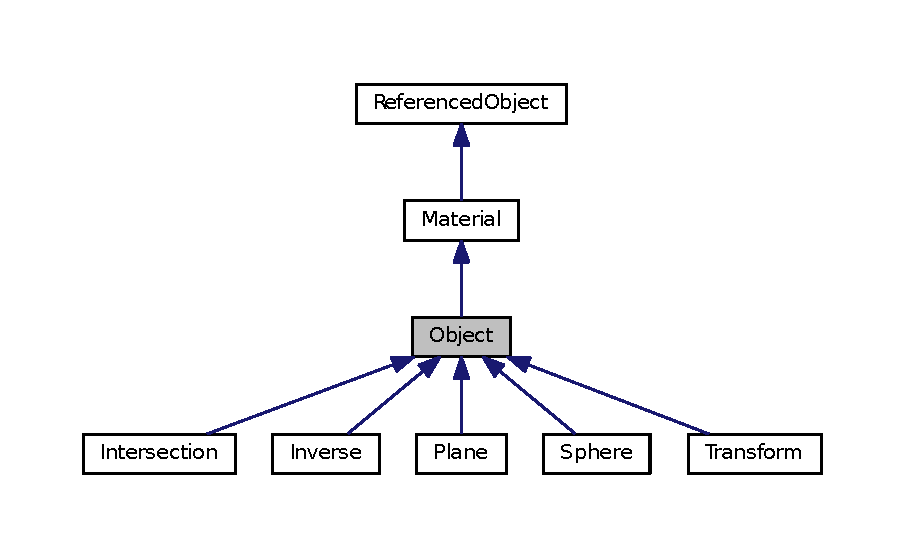
\includegraphics[width=350pt]{class_object__inherit__graph}
\end{center}
\end{figure}


Collaboration diagram for Object\+:
\nopagebreak
\begin{figure}[H]
\begin{center}
\leavevmode
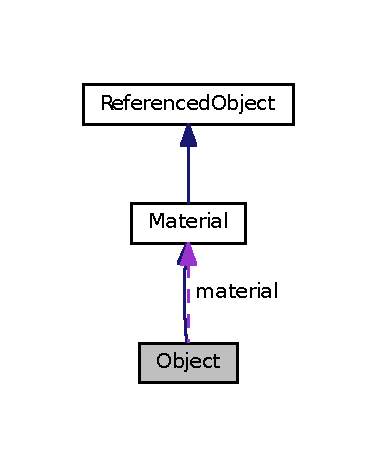
\includegraphics[width=181pt]{class_object__coll__graph}
\end{center}
\end{figure}
\subsection*{Public Member Functions}
\begin{DoxyCompactItemize}
\item 
{\bf Object} ()
\item 
virtual {\bf $\sim$\+Object} ()=0
\begin{DoxyCompactList}\small\item\em All objects must have a virtual destructor so that they can be deallocated properly and to dereference any contained objects. \end{DoxyCompactList}\item 
virtual double {\bf line\+Test} (double origin[3], double direction[3], double max\+Distance)=0
\begin{DoxyCompactList}\small\item\em Must do the line intersection test and return the closest distance in which a ray originating in origin with given direction intersects the object -\/ if such a point exists closer than max\+Distance. \end{DoxyCompactList}\item 
virtual void {\bf get\+Normal} (double point[3], double normal[3])=0
\begin{DoxyCompactList}\small\item\em Compute the normal of the object at the given point. \end{DoxyCompactList}\item 
virtual bool {\bf is\+Inside} (double point[3])=0
\begin{DoxyCompactList}\small\item\em Tests if a point is inside the object or not. \end{DoxyCompactList}\item 
virtual void {\bf set\+Material} ({\bf Material} $\ast${\bf material})
\begin{DoxyCompactList}\small\item\em Sets up a default material to use for this object. \end{DoxyCompactList}\item 
virtual void {\bf get\+Lighting\+Properties} (double point[3], {\bf Lighting\+Properties} $\ast$props, double normal[3])
\begin{DoxyCompactList}\small\item\em Default material handling that queries the default material given for this object. \end{DoxyCompactList}\end{DoxyCompactItemize}
\subsection*{Protected Attributes}
\begin{DoxyCompactItemize}
\item 
{\bf Material} $\ast$ {\bf material}
\begin{DoxyCompactList}\small\item\em \doxyref{Material}{p.}{class_material} used by the default get\+Lighting\+Properties function. \end{DoxyCompactList}\end{DoxyCompactItemize}


\subsection{Detailed Description}
Abstract base class for all renderable objects. 

Each concrete instance of this class must contain virtual functions that are used to perform line tests, computing normals and lighting properties. 

Definition at line 39 of file object.\+h.



\subsection{Constructor \& Destructor Documentation}
\index{Object@{Object}!Object@{Object}}
\index{Object@{Object}!Object@{Object}}
\subsubsection[{Object}]{\setlength{\rightskip}{0pt plus 5cm}Object\+::\+Object (
\begin{DoxyParamCaption}
{}
\end{DoxyParamCaption}
)}\label{class_object_a40860402e64d8008fb42329df7097cdb}


Definition at line 29 of file object.\+cc.



References material.

\index{Object@{Object}!````~Object@{$\sim$\+Object}}
\index{````~Object@{$\sim$\+Object}!Object@{Object}}
\subsubsection[{$\sim$\+Object}]{\setlength{\rightskip}{0pt plus 5cm}Object\+::$\sim$\+Object (
\begin{DoxyParamCaption}
{}
\end{DoxyParamCaption}
)\hspace{0.3cm}{\ttfamily [pure virtual]}}\label{class_object_a6345bacd6b9d1e2814db2dc178f68716}


All objects must have a virtual destructor so that they can be deallocated properly and to dereference any contained objects. 



Definition at line 30 of file object.\+cc.



References Referenced\+Object\+::dereference(), and material.



\subsection{Member Function Documentation}
\index{Object@{Object}!get\+Lighting\+Properties@{get\+Lighting\+Properties}}
\index{get\+Lighting\+Properties@{get\+Lighting\+Properties}!Object@{Object}}
\subsubsection[{get\+Lighting\+Properties}]{\setlength{\rightskip}{0pt plus 5cm}void Object\+::get\+Lighting\+Properties (
\begin{DoxyParamCaption}
\item[{double}]{point[3], }
\item[{{\bf Lighting\+Properties} $\ast$}]{props, }
\item[{double}]{normal[3]}
\end{DoxyParamCaption}
)\hspace{0.3cm}{\ttfamily [virtual]}}\label{class_object_a510171215bdf364cc0bf8f72336039b9}


Default material handling that queries the default material given for this object. 



Implements {\bf Material} \doxyref{}{p.}{class_material_ab61e7df6a740ad2ad3a82700005982bd}.



Reimplemented in {\bf Inverse} \doxyref{}{p.}{class_inverse_abedf66c2607143f237f913187ecfdc40}, {\bf Transform} \doxyref{}{p.}{class_transform_a6759fe52b87d9113c48c0414824ac067}, and {\bf Intersection} \doxyref{}{p.}{class_intersection_aeaf604c0cdbef2d4c2a0f2087287ead8}.



Definition at line 36 of file object.\+cc.



References Material\+::get\+Lighting\+Properties(), and material.



Referenced by Transform\+::get\+Lighting\+Properties(), and Raytracer\+::raytrace().

\index{Object@{Object}!get\+Normal@{get\+Normal}}
\index{get\+Normal@{get\+Normal}!Object@{Object}}
\subsubsection[{get\+Normal}]{\setlength{\rightskip}{0pt plus 5cm}virtual void Object\+::get\+Normal (
\begin{DoxyParamCaption}
\item[{double}]{point[3], }
\item[{double}]{normal[3]}
\end{DoxyParamCaption}
)\hspace{0.3cm}{\ttfamily [pure virtual]}}\label{class_object_a22c15ace5725e2577dbb187265bd3201}


Compute the normal of the object at the given point. 

Result is not guaranteed to be of unit length. 

Implemented in {\bf Inverse} \doxyref{}{p.}{class_inverse_aead295a76d1bd7d8478fc0e32710c84f}, {\bf Intersection} \doxyref{}{p.}{class_intersection_aca5201537e1f12305142be681b0e0b47}, {\bf Transform} \doxyref{}{p.}{class_transform_ab9b4a86bde00d015be3ee563a072ceeb}, {\bf Sphere} \doxyref{}{p.}{class_sphere_a36b26e53cef4b521c97df51fac315c68}, and {\bf Plane} \doxyref{}{p.}{class_plane_a323f52af3edd8c55ffd23324a61da5ec}.



Referenced by Transform\+::get\+Normal(), and Raytracer\+::raytrace().

\index{Object@{Object}!is\+Inside@{is\+Inside}}
\index{is\+Inside@{is\+Inside}!Object@{Object}}
\subsubsection[{is\+Inside}]{\setlength{\rightskip}{0pt plus 5cm}virtual bool Object\+::is\+Inside (
\begin{DoxyParamCaption}
\item[{double}]{point[3]}
\end{DoxyParamCaption}
)\hspace{0.3cm}{\ttfamily [pure virtual]}}\label{class_object_a652359286747bf237cb2d4d0a802bd18}


Tests if a point is inside the object or not. 



Implemented in {\bf Inverse} \doxyref{}{p.}{class_inverse_af3747e94047e18d4eff0fc61a92bf915}, {\bf Intersection} \doxyref{}{p.}{class_intersection_acbba7803bcd3928967fd675992a8ae96}, {\bf Transform} \doxyref{}{p.}{class_transform_acf224e03c58e2923df817808f66f1cd0}, {\bf Sphere} \doxyref{}{p.}{class_sphere_a25cf6b133c99f57aa23380c4511507cf}, and {\bf Plane} \doxyref{}{p.}{class_plane_a905978138dff21894a040eebee557b16}.



Referenced by Transform\+::is\+Inside().

\index{Object@{Object}!line\+Test@{line\+Test}}
\index{line\+Test@{line\+Test}!Object@{Object}}
\subsubsection[{line\+Test}]{\setlength{\rightskip}{0pt plus 5cm}virtual double Object\+::line\+Test (
\begin{DoxyParamCaption}
\item[{double}]{origin[3], }
\item[{double}]{direction[3], }
\item[{double}]{max\+Distance}
\end{DoxyParamCaption}
)\hspace{0.3cm}{\ttfamily [pure virtual]}}\label{class_object_a1bfd7ffbccda28c67d8a537393113a7e}


Must do the line intersection test and return the closest distance in which a ray originating in origin with given direction intersects the object -\/ if such a point exists closer than max\+Distance. 

Returns distance M\+A\+X\+\_\+\+D\+I\+S\+T\+A\+N\+C\+E if no such intersection exists.

Direction is not neccessarily a vector of unit length, and distances are measured in multiples of this vector. 

Implemented in {\bf Inverse} \doxyref{}{p.}{class_inverse_a7cd665a12ccf90142526965dfe416d1f}, {\bf Intersection} \doxyref{}{p.}{class_intersection_acadaeb4e35a52f4d1ff80769586921ff}, {\bf Transform} \doxyref{}{p.}{class_transform_ab2e6df43a4e87522a6e446b10cd67ca5}, {\bf Sphere} \doxyref{}{p.}{class_sphere_a138bf6427c11475d7b42f9debd6a1971}, and {\bf Plane} \doxyref{}{p.}{class_plane_acec0051b3d12e8ddd1e475de3f4ad9de}.



Referenced by Transform\+::line\+Test(), and Raytracer\+::raytrace().

\index{Object@{Object}!set\+Material@{set\+Material}}
\index{set\+Material@{set\+Material}!Object@{Object}}
\subsubsection[{set\+Material}]{\setlength{\rightskip}{0pt plus 5cm}void Object\+::set\+Material (
\begin{DoxyParamCaption}
\item[{{\bf Material} $\ast$}]{material}
\end{DoxyParamCaption}
)\hspace{0.3cm}{\ttfamily [virtual]}}\label{class_object_a239c2cad955282c6294da3d35be48fbd}


Sets up a default material to use for this object. 



Definition at line 31 of file object.\+cc.



References Referenced\+Object\+::dereference(), material, and Referenced\+Object\+::reference().



Referenced by main().



\subsection{Member Data Documentation}
\index{Object@{Object}!material@{material}}
\index{material@{material}!Object@{Object}}
\subsubsection[{material}]{\setlength{\rightskip}{0pt plus 5cm}{\bf Material}$\ast$ Object\+::material\hspace{0.3cm}{\ttfamily [protected]}}\label{class_object_af475bd962d08ec97add4497e92436076}


\doxyref{Material}{p.}{class_material} used by the default get\+Lighting\+Properties function. 



Definition at line 71 of file object.\+h.



Referenced by Transform\+::get\+Lighting\+Properties(), get\+Lighting\+Properties(), Object(), set\+Material(), and $\sim$\+Object().



The documentation for this class was generated from the following files\+:\begin{DoxyCompactItemize}
\item 
{\bf object.\+h}\item 
{\bf object.\+cc}\end{DoxyCompactItemize}

\section{Plane Class Reference}
\label{class_plane}\index{Plane@{Plane}}


An infinite plane with given normal and offset from origo.  




{\ttfamily \#include $<$plane.\+h$>$}



Inheritance diagram for Plane\+:
\nopagebreak
\begin{figure}[H]
\begin{center}
\leavevmode
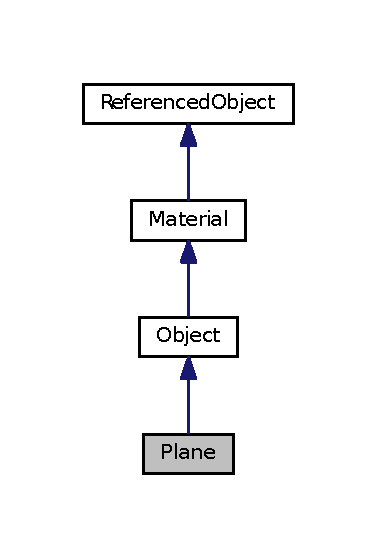
\includegraphics[width=181pt]{class_plane__inherit__graph}
\end{center}
\end{figure}


Collaboration diagram for Plane\+:
\nopagebreak
\begin{figure}[H]
\begin{center}
\leavevmode
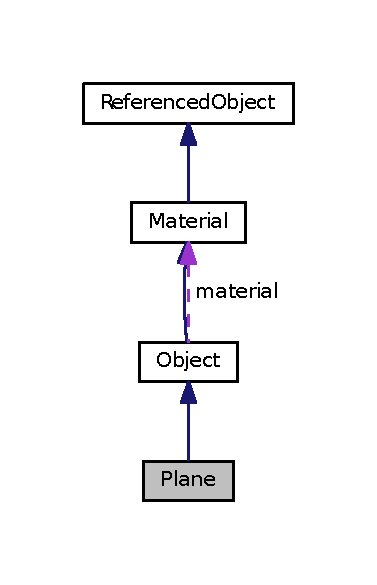
\includegraphics[width=181pt]{class_plane__coll__graph}
\end{center}
\end{figure}
\subsection*{Public Member Functions}
\begin{DoxyCompactItemize}
\item 
{\bf Plane} (double {\bf normal}[3], double {\bf offset})
\item 
{\bf $\sim$\+Plane} ()
\item 
double {\bf line\+Test} (double origin[3], double direction[3], double max\+Distance)
\begin{DoxyCompactList}\small\item\em Must do the line intersection test and return the closest distance in which a ray originating in origin with given direction intersects the object -\/ if such a point exists closer than max\+Distance. \end{DoxyCompactList}\item 
void {\bf get\+Normal} (double point[3], double {\bf normal}[3])
\begin{DoxyCompactList}\small\item\em Compute the normal of the object at the given point. \end{DoxyCompactList}\item 
bool {\bf is\+Inside} (double point[3])
\begin{DoxyCompactList}\small\item\em Tests if a point is inside the object or not. \end{DoxyCompactList}\end{DoxyCompactItemize}
\subsection*{Private Attributes}
\begin{DoxyCompactItemize}
\item 
double {\bf normal} [3]
\item 
double {\bf offset}
\end{DoxyCompactItemize}
\subsection*{Additional Inherited Members}


\subsection{Detailed Description}
An infinite plane with given normal and offset from origo. 



Definition at line 32 of file plane.\+h.



\subsection{Constructor \& Destructor Documentation}
\index{Plane@{Plane}!Plane@{Plane}}
\index{Plane@{Plane}!Plane@{Plane}}
\subsubsection[{Plane}]{\setlength{\rightskip}{0pt plus 5cm}Plane\+::\+Plane (
\begin{DoxyParamCaption}
\item[{double}]{normal[3], }
\item[{double}]{offset}
\end{DoxyParamCaption}
)}\label{class_plane_a1db2a39c0d19550c86dd0c5c9474682e}


Definition at line 27 of file plane.\+cc.



References assign(), and offset.

\index{Plane@{Plane}!````~Plane@{$\sim$\+Plane}}
\index{````~Plane@{$\sim$\+Plane}!Plane@{Plane}}
\subsubsection[{$\sim$\+Plane}]{\setlength{\rightskip}{0pt plus 5cm}Plane\+::$\sim$\+Plane (
\begin{DoxyParamCaption}
{}
\end{DoxyParamCaption}
)}\label{class_plane_a69abd86051c880dcb44b249ad10c4436}


Definition at line 31 of file plane.\+cc.



\subsection{Member Function Documentation}
\index{Plane@{Plane}!get\+Normal@{get\+Normal}}
\index{get\+Normal@{get\+Normal}!Plane@{Plane}}
\subsubsection[{get\+Normal}]{\setlength{\rightskip}{0pt plus 5cm}void Plane\+::get\+Normal (
\begin{DoxyParamCaption}
\item[{double}]{point[3], }
\item[{double}]{normal[3]}
\end{DoxyParamCaption}
)\hspace{0.3cm}{\ttfamily [virtual]}}\label{class_plane_a323f52af3edd8c55ffd23324a61da5ec}


Compute the normal of the object at the given point. 

Result is not guaranteed to be of unit length. 

Implements {\bf Object} \doxyref{}{p.}{class_object_a22c15ace5725e2577dbb187265bd3201}.



Definition at line 48 of file plane.\+cc.



References assign().

\index{Plane@{Plane}!is\+Inside@{is\+Inside}}
\index{is\+Inside@{is\+Inside}!Plane@{Plane}}
\subsubsection[{is\+Inside}]{\setlength{\rightskip}{0pt plus 5cm}bool Plane\+::is\+Inside (
\begin{DoxyParamCaption}
\item[{double}]{point[3]}
\end{DoxyParamCaption}
)\hspace{0.3cm}{\ttfamily [virtual]}}\label{class_plane_a905978138dff21894a040eebee557b16}


Tests if a point is inside the object or not. 



Implements {\bf Object} \doxyref{}{p.}{class_object_a652359286747bf237cb2d4d0a802bd18}.



Definition at line 52 of file plane.\+cc.



References dot\+Product(), normal, and offset.

\index{Plane@{Plane}!line\+Test@{line\+Test}}
\index{line\+Test@{line\+Test}!Plane@{Plane}}
\subsubsection[{line\+Test}]{\setlength{\rightskip}{0pt plus 5cm}double Plane\+::line\+Test (
\begin{DoxyParamCaption}
\item[{double}]{origin[3], }
\item[{double}]{direction[3], }
\item[{double}]{max\+Distance}
\end{DoxyParamCaption}
)\hspace{0.3cm}{\ttfamily [virtual]}}\label{class_plane_acec0051b3d12e8ddd1e475de3f4ad9de}


Must do the line intersection test and return the closest distance in which a ray originating in origin with given direction intersects the object -\/ if such a point exists closer than max\+Distance. 

Returns distance M\+A\+X\+\_\+\+D\+I\+S\+T\+A\+N\+C\+E if no such intersection exists.

Direction is not neccessarily a vector of unit length, and distances are measured in multiples of this vector. 

Implements {\bf Object} \doxyref{}{p.}{class_object_a1bfd7ffbccda28c67d8a537393113a7e}.



Definition at line 33 of file plane.\+cc.



References debug\+This\+Pixel, dot\+Product(), M\+A\+X\+\_\+\+D\+I\+S\+T\+A\+N\+C\+E, normal, offset, and print\+Debug\+Indentation().



\subsection{Member Data Documentation}
\index{Plane@{Plane}!normal@{normal}}
\index{normal@{normal}!Plane@{Plane}}
\subsubsection[{normal}]{\setlength{\rightskip}{0pt plus 5cm}double Plane\+::normal[3]\hspace{0.3cm}{\ttfamily [private]}}\label{class_plane_ad7347d52010f30316c0eca946b3d43e2}


Definition at line 42 of file plane.\+h.



Referenced by is\+Inside(), and line\+Test().

\index{Plane@{Plane}!offset@{offset}}
\index{offset@{offset}!Plane@{Plane}}
\subsubsection[{offset}]{\setlength{\rightskip}{0pt plus 5cm}double Plane\+::offset\hspace{0.3cm}{\ttfamily [private]}}\label{class_plane_aa4fdb4c5c50553d97341b030cb900736}


Definition at line 42 of file plane.\+h.



Referenced by is\+Inside(), line\+Test(), and Plane().



The documentation for this class was generated from the following files\+:\begin{DoxyCompactItemize}
\item 
{\bf plane.\+h}\item 
{\bf plane.\+cc}\end{DoxyCompactItemize}

\section{Raytracer Class Reference}
\label{class_raytracer}\index{Raytracer@{Raytracer}}


Main class for performing all raytracing operations.  




{\ttfamily \#include $<$raytracer.\+h$>$}



Collaboration diagram for Raytracer\+:
\nopagebreak
\begin{figure}[H]
\begin{center}
\leavevmode
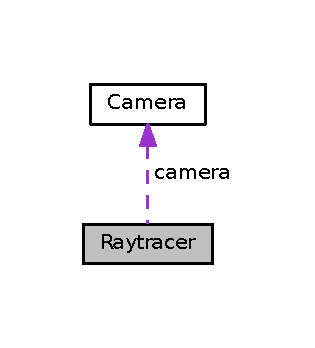
\includegraphics[width=151pt]{class_raytracer__coll__graph}
\end{center}
\end{figure}
\subsection*{Public Member Functions}
\begin{DoxyCompactItemize}
\item 
{\bf Raytracer} ()
\item 
{\bf $\sim$\+Raytracer} ()
\item 
void {\bf set\+Background} (double[3])
\begin{DoxyCompactList}\small\item\em Sets the background colour of the scene, ie. \end{DoxyCompactList}\item 
void {\bf set\+Ambient\+Light} (double[3])
\begin{DoxyCompactList}\small\item\em Sets the global ambient light in the scene. \end{DoxyCompactList}\item 
void {\bf add\+Light} ({\bf Light} $\ast$)
\begin{DoxyCompactList}\small\item\em Adds a lightsource to the scene. \end{DoxyCompactList}\item 
void {\bf add\+Object} ({\bf Object} $\ast$)
\begin{DoxyCompactList}\small\item\em Adds an object to the scene. \end{DoxyCompactList}\item 
void {\bf set\+Camera} ({\bf Camera} $\ast$)
\begin{DoxyCompactList}\small\item\em Sets the camera object to be used when determining origin of the rays. \end{DoxyCompactList}\item 
{\bf Camera} $\ast$ {\bf get\+Camera} ()
\begin{DoxyCompactList}\small\item\em Gives the camera object currently used. \end{DoxyCompactList}\item 
void {\bf raytrace} (double origin[3], double direction[3], double rgb[3], double contribution)
\begin{DoxyCompactList}\small\item\em Basic raytracing routine that computes a colour to assign to a ray originating in origin with the given direction. \end{DoxyCompactList}\item 
void {\bf raytrace} (int x, int y, double rgb[3])
\begin{DoxyCompactList}\small\item\em Special case of general raytracing routine for screen pixel X,Y. \end{DoxyCompactList}\end{DoxyCompactItemize}
\subsection*{Private Attributes}
\begin{DoxyCompactItemize}
\item 
{\bf Camera} $\ast$ {\bf camera}
\item 
double {\bf background} [3]
\item 
double {\bf ambient\+Light} [3]
\item 
class std\+::set$<$ {\bf Light} $\ast$ $>$ $\ast$ {\bf lights}
\item 
class std\+::set$<$ {\bf Object} $\ast$ $>$ $\ast$ {\bf objects}
\end{DoxyCompactItemize}


\subsection{Detailed Description}
Main class for performing all raytracing operations. 

To use, instantiate this class and give it a scene graph using the add\+Object and add\+Light operations. Also pass it a camera object using the set\+Camera function and give global lighting properties using set\+Background nad set\+Ambient\+Light.

Once ready to use, the actual raytracing operation can be performed by calling the raytracer function for every pixel on the screen.

Note that all objects are asssumed to be reentrant during the raytracring (ie. they should not change any internal state variables), and that updates on them should only be made in between frames. 

Definition at line 56 of file raytracer.\+h.



\subsection{Constructor \& Destructor Documentation}
\index{Raytracer@{Raytracer}!Raytracer@{Raytracer}}
\index{Raytracer@{Raytracer}!Raytracer@{Raytracer}}
\subsubsection[{Raytracer}]{\setlength{\rightskip}{0pt plus 5cm}Raytracer\+::\+Raytracer (
\begin{DoxyParamCaption}
{}
\end{DoxyParamCaption}
)}\label{class_raytracer_ab012a6a83fb2ed05aa52993a9f6c2d53}


Definition at line 31 of file raytracer.\+cc.



References zero().



Referenced by main().

\index{Raytracer@{Raytracer}!````~Raytracer@{$\sim$\+Raytracer}}
\index{````~Raytracer@{$\sim$\+Raytracer}!Raytracer@{Raytracer}}
\subsubsection[{$\sim$\+Raytracer}]{\setlength{\rightskip}{0pt plus 5cm}Raytracer\+::$\sim$\+Raytracer (
\begin{DoxyParamCaption}
{}
\end{DoxyParamCaption}
)}\label{class_raytracer_a610ba0d74edf864c8ed78c5d85c4480a}


Definition at line 37 of file raytracer.\+cc.



\subsection{Member Function Documentation}
\index{Raytracer@{Raytracer}!add\+Light@{add\+Light}}
\index{add\+Light@{add\+Light}!Raytracer@{Raytracer}}
\subsubsection[{add\+Light}]{\setlength{\rightskip}{0pt plus 5cm}void Raytracer\+::add\+Light (
\begin{DoxyParamCaption}
\item[{{\bf Light} $\ast$}]{light}
\end{DoxyParamCaption}
)}\label{class_raytracer_a5e53831c2c52c3279b1a24ffef89c23f}


Adds a lightsource to the scene. 



Definition at line 58 of file raytracer.\+cc.



References Referenced\+Object\+::reference().



Referenced by main().

\index{Raytracer@{Raytracer}!add\+Object@{add\+Object}}
\index{add\+Object@{add\+Object}!Raytracer@{Raytracer}}
\subsubsection[{add\+Object}]{\setlength{\rightskip}{0pt plus 5cm}void Raytracer\+::add\+Object (
\begin{DoxyParamCaption}
\item[{{\bf Object} $\ast$}]{object}
\end{DoxyParamCaption}
)}\label{class_raytracer_ae03ca1a9a2c5f75744905a0c1bbc9734}


Adds an object to the scene. 



Definition at line 54 of file raytracer.\+cc.



Referenced by main().

\index{Raytracer@{Raytracer}!get\+Camera@{get\+Camera}}
\index{get\+Camera@{get\+Camera}!Raytracer@{Raytracer}}
\subsubsection[{get\+Camera}]{\setlength{\rightskip}{0pt plus 5cm}{\bf Camera} $\ast$ Raytracer\+::get\+Camera (
\begin{DoxyParamCaption}
{}
\end{DoxyParamCaption}
)}\label{class_raytracer_a84ef76a6d46b258ccc7f4b93e9cff012}


Gives the camera object currently used. 



Definition at line 63 of file raytracer.\+cc.



Referenced by do\+Redraw().

\index{Raytracer@{Raytracer}!raytrace@{raytrace}}
\index{raytrace@{raytrace}!Raytracer@{Raytracer}}
\subsubsection[{raytrace}]{\setlength{\rightskip}{0pt plus 5cm}void Raytracer\+::raytrace (
\begin{DoxyParamCaption}
\item[{double}]{origin[3], }
\item[{double}]{direction[3], }
\item[{double}]{rgb[3], }
\item[{double}]{contribution}
\end{DoxyParamCaption}
)}\label{class_raytracer_aa1ab546300704b6db468549d1b60ede0}


Basic raytracing routine that computes a colour to assign to a ray originating in origin with the given direction. 

If no intersecting objects are found then it assigns the background colour to the vector rgb, otherwise the result of doing the light computations and recursive raytracing from the intersection point.

Contribution is a hint for how much the resuling colours will contribute to the screen pixels and can be used to limit recursion. 

Definition at line 69 of file raytracer.\+cc.



References Lighting\+Properties\+::ambient, Light\+::colour, debug\+Indentation, debug\+This\+Pixel, Lighting\+Properties\+::diffuse, dot\+Product(), Object\+::get\+Lighting\+Properties(), Object\+::get\+Normal(), length(), Object\+::line\+Test(), M\+A\+X\+\_\+\+D\+I\+S\+T\+A\+N\+C\+E, normalize(), Light\+::position, print\+Debug\+Indentation(), Lighting\+Properties\+::reflection, Lighting\+Properties\+::shininess, Lighting\+Properties\+::specular, and sub().



Referenced by do\+Redraw().

\index{Raytracer@{Raytracer}!raytrace@{raytrace}}
\index{raytrace@{raytrace}!Raytracer@{Raytracer}}
\subsubsection[{raytrace}]{\setlength{\rightskip}{0pt plus 5cm}void Raytracer\+::raytrace (
\begin{DoxyParamCaption}
\item[{int}]{x, }
\item[{int}]{y, }
\item[{double}]{rgb[3]}
\end{DoxyParamCaption}
)}\label{class_raytracer_ae74fb4d0e5843de85e638c8d4a54e423}


Special case of general raytracing routine for screen pixel X,Y. 

Fetches the origin/direction from the current camera settings. 

Definition at line 64 of file raytracer.\+cc.



References screen\+Height, and screen\+Width.

\index{Raytracer@{Raytracer}!set\+Ambient\+Light@{set\+Ambient\+Light}}
\index{set\+Ambient\+Light@{set\+Ambient\+Light}!Raytracer@{Raytracer}}
\subsubsection[{set\+Ambient\+Light}]{\setlength{\rightskip}{0pt plus 5cm}void Raytracer\+::set\+Ambient\+Light (
\begin{DoxyParamCaption}
\item[{double}]{col[3]}
\end{DoxyParamCaption}
)}\label{class_raytracer_ad575fe4aaf08119db97118e60e481a13}


Sets the global ambient light in the scene. 



Definition at line 52 of file raytracer.\+cc.



References assign().



Referenced by main().

\index{Raytracer@{Raytracer}!set\+Background@{set\+Background}}
\index{set\+Background@{set\+Background}!Raytracer@{Raytracer}}
\subsubsection[{set\+Background}]{\setlength{\rightskip}{0pt plus 5cm}void Raytracer\+::set\+Background (
\begin{DoxyParamCaption}
\item[{double}]{col[3]}
\end{DoxyParamCaption}
)}\label{class_raytracer_ad5bbcd47429ca7822a3cb9226ec6c81a}


Sets the background colour of the scene, ie. 

the colour used for all pixels that hit no object. 

Definition at line 51 of file raytracer.\+cc.



References assign().

\index{Raytracer@{Raytracer}!set\+Camera@{set\+Camera}}
\index{set\+Camera@{set\+Camera}!Raytracer@{Raytracer}}
\subsubsection[{set\+Camera}]{\setlength{\rightskip}{0pt plus 5cm}void Raytracer\+::set\+Camera (
\begin{DoxyParamCaption}
\item[{{\bf Camera} $\ast$}]{cam}
\end{DoxyParamCaption}
)}\label{class_raytracer_a48979448b65a995721450c8c7ded9f19}


Sets the camera object to be used when determining origin of the rays. 



Definition at line 62 of file raytracer.\+cc.



Referenced by main().



\subsection{Member Data Documentation}
\index{Raytracer@{Raytracer}!ambient\+Light@{ambient\+Light}}
\index{ambient\+Light@{ambient\+Light}!Raytracer@{Raytracer}}
\subsubsection[{ambient\+Light}]{\setlength{\rightskip}{0pt plus 5cm}double Raytracer\+::ambient\+Light[3]\hspace{0.3cm}{\ttfamily [private]}}\label{class_raytracer_a7912e30ac04157900286f2fa6eaf8ae7}


Definition at line 95 of file raytracer.\+h.



Referenced by main().

\index{Raytracer@{Raytracer}!background@{background}}
\index{background@{background}!Raytracer@{Raytracer}}
\subsubsection[{background}]{\setlength{\rightskip}{0pt plus 5cm}double Raytracer\+::background[3]\hspace{0.3cm}{\ttfamily [private]}}\label{class_raytracer_a4780e0feac28d575a53d7981113467ad}


Definition at line 94 of file raytracer.\+h.

\index{Raytracer@{Raytracer}!camera@{camera}}
\index{camera@{camera}!Raytracer@{Raytracer}}
\subsubsection[{camera}]{\setlength{\rightskip}{0pt plus 5cm}{\bf Camera}$\ast$ Raytracer\+::camera\hspace{0.3cm}{\ttfamily [private]}}\label{class_raytracer_aa56a6383a51f5b4f4142ff1223e7d6e7}


Definition at line 93 of file raytracer.\+h.



Referenced by do\+Redraw().

\index{Raytracer@{Raytracer}!lights@{lights}}
\index{lights@{lights}!Raytracer@{Raytracer}}
\subsubsection[{lights}]{\setlength{\rightskip}{0pt plus 5cm}class std\+::set$<$ {\bf Light} $\ast$ $>$$\ast$ Raytracer\+::lights\hspace{0.3cm}{\ttfamily [private]}}\label{class_raytracer_aec6b370de6983fda41b3705664bf2841}


Definition at line 97 of file raytracer.\+h.

\index{Raytracer@{Raytracer}!objects@{objects}}
\index{objects@{objects}!Raytracer@{Raytracer}}
\subsubsection[{objects}]{\setlength{\rightskip}{0pt plus 5cm}class std\+::set$<$ {\bf Object} $\ast$ $>$$\ast$ Raytracer\+::objects\hspace{0.3cm}{\ttfamily [private]}}\label{class_raytracer_ad2035caf15bcdf69dad408afcb03ea52}


Definition at line 98 of file raytracer.\+h.



The documentation for this class was generated from the following files\+:\begin{DoxyCompactItemize}
\item 
{\bf raytracer.\+h}\item 
{\bf raytracer.\+cc}\end{DoxyCompactItemize}

\section{Referenced\+Object Class Reference}
\label{class_referenced_object}\index{Referenced\+Object@{Referenced\+Object}}


Base class for all objects which use a reference counter for memory management.  




{\ttfamily \#include $<$referenced.\+h$>$}



Inheritance diagram for Referenced\+Object\+:
\nopagebreak
\begin{figure}[H]
\begin{center}
\leavevmode
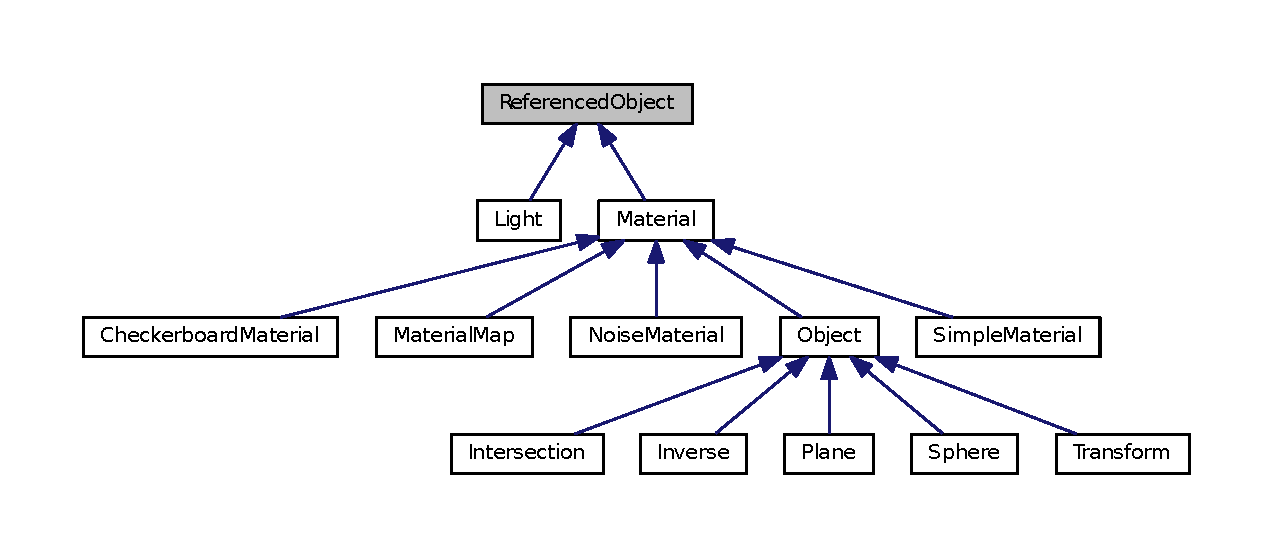
\includegraphics[width=350pt]{class_referenced_object__inherit__graph}
\end{center}
\end{figure}
\subsection*{Public Member Functions}
\begin{DoxyCompactItemize}
\item 
{\bf Referenced\+Object} ()
\item 
virtual {\bf $\sim$\+Referenced\+Object} ()
\item 
void {\bf reference} ()
\begin{DoxyCompactList}\small\item\em Call when an object reference is added to memory. \end{DoxyCompactList}\item 
void {\bf dereference} ()
\begin{DoxyCompactList}\small\item\em Call when an object is dereferenced. \end{DoxyCompactList}\end{DoxyCompactItemize}
\subsection*{Private Attributes}
\begin{DoxyCompactItemize}
\item 
int {\bf reference\+Counter}
\end{DoxyCompactItemize}


\subsection{Detailed Description}
Base class for all objects which use a reference counter for memory management. 



Definition at line 30 of file referenced.\+h.



\subsection{Constructor \& Destructor Documentation}
\index{Referenced\+Object@{Referenced\+Object}!Referenced\+Object@{Referenced\+Object}}
\index{Referenced\+Object@{Referenced\+Object}!Referenced\+Object@{Referenced\+Object}}
\subsubsection[{Referenced\+Object}]{\setlength{\rightskip}{0pt plus 5cm}Referenced\+Object\+::\+Referenced\+Object (
\begin{DoxyParamCaption}
{}
\end{DoxyParamCaption}
)}\label{class_referenced_object_af6e810408b0eb5855dbb467065016d79}


Definition at line 28 of file referenced.\+cc.



References reference\+Counter.

\index{Referenced\+Object@{Referenced\+Object}!````~Referenced\+Object@{$\sim$\+Referenced\+Object}}
\index{````~Referenced\+Object@{$\sim$\+Referenced\+Object}!Referenced\+Object@{Referenced\+Object}}
\subsubsection[{$\sim$\+Referenced\+Object}]{\setlength{\rightskip}{0pt plus 5cm}Referenced\+Object\+::$\sim$\+Referenced\+Object (
\begin{DoxyParamCaption}
{}
\end{DoxyParamCaption}
)\hspace{0.3cm}{\ttfamily [virtual]}}\label{class_referenced_object_a7f91d5df8ecc65e0edb25ef05b36c58b}


Definition at line 31 of file referenced.\+cc.



\subsection{Member Function Documentation}
\index{Referenced\+Object@{Referenced\+Object}!dereference@{dereference}}
\index{dereference@{dereference}!Referenced\+Object@{Referenced\+Object}}
\subsubsection[{dereference}]{\setlength{\rightskip}{0pt plus 5cm}void Referenced\+Object\+::dereference (
\begin{DoxyParamCaption}
{}
\end{DoxyParamCaption}
)}\label{class_referenced_object_a1b140008d6095b8590c59671bf5515d8}


Call when an object is dereferenced. 

Decreases the reference counter by one and deallocates the memory for the objectif neccessary. 

Definition at line 33 of file referenced.\+cc.



References reference\+Counter.



Referenced by Object\+::set\+Material(), Object\+::$\sim$\+Object(), and Transform\+::$\sim$\+Transform().

\index{Referenced\+Object@{Referenced\+Object}!reference@{reference}}
\index{reference@{reference}!Referenced\+Object@{Referenced\+Object}}
\subsubsection[{reference}]{\setlength{\rightskip}{0pt plus 5cm}void Referenced\+Object\+::reference (
\begin{DoxyParamCaption}
{}
\end{DoxyParamCaption}
)}\label{class_referenced_object_a0fc8392b9b02ce8203f7e01ee150397d}


Call when an object reference is added to memory. 

Increases the reference counter by one 

Definition at line 32 of file referenced.\+cc.



References reference\+Counter.



Referenced by Raytracer\+::add\+Light(), Inverse\+::\+Inverse(), Object\+::set\+Material(), and Transform\+::\+Transform().



\subsection{Member Data Documentation}
\index{Referenced\+Object@{Referenced\+Object}!reference\+Counter@{reference\+Counter}}
\index{reference\+Counter@{reference\+Counter}!Referenced\+Object@{Referenced\+Object}}
\subsubsection[{reference\+Counter}]{\setlength{\rightskip}{0pt plus 5cm}int Referenced\+Object\+::reference\+Counter\hspace{0.3cm}{\ttfamily [private]}}\label{class_referenced_object_ae69c5359c130b544300b7ce189fd1d39}


Definition at line 42 of file referenced.\+h.



Referenced by dereference(), reference(), and Referenced\+Object().



The documentation for this class was generated from the following files\+:\begin{DoxyCompactItemize}
\item 
{\bf referenced.\+h}\item 
{\bf referenced.\+cc}\end{DoxyCompactItemize}

\section{Simple\+Material Class Reference}
\label{class_simple_material}\index{Simple\+Material@{Simple\+Material}}


Implements a simple material with the same properties over all of the whole object.  




{\ttfamily \#include $<$material.\+h$>$}



Inheritance diagram for Simple\+Material\+:
\nopagebreak
\begin{figure}[H]
\begin{center}
\leavevmode
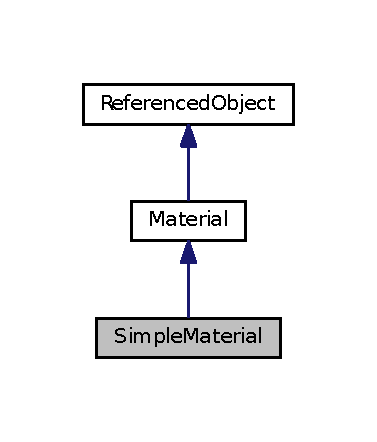
\includegraphics[width=181pt]{class_simple_material__inherit__graph}
\end{center}
\end{figure}


Collaboration diagram for Simple\+Material\+:
\nopagebreak
\begin{figure}[H]
\begin{center}
\leavevmode
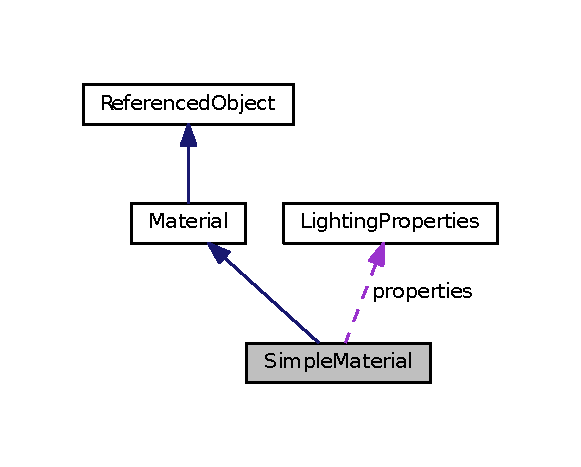
\includegraphics[width=279pt]{class_simple_material__coll__graph}
\end{center}
\end{figure}
\subsection*{Public Member Functions}
\begin{DoxyCompactItemize}
\item 
{\bf Simple\+Material} ({\bf Lighting\+Properties} $\ast$)
\item 
virtual void {\bf get\+Lighting\+Properties} (double point[3], {\bf Lighting\+Properties} $\ast$props, double normal[3])
\begin{DoxyCompactList}\small\item\em Returns the lighting properites at a certain point. \end{DoxyCompactList}\end{DoxyCompactItemize}
\subsection*{Private Attributes}
\begin{DoxyCompactItemize}
\item 
{\bf Lighting\+Properties} {\bf properties}
\end{DoxyCompactItemize}


\subsection{Detailed Description}
Implements a simple material with the same properties over all of the whole object. 



Definition at line 63 of file material.\+h.



\subsection{Constructor \& Destructor Documentation}
\index{Simple\+Material@{Simple\+Material}!Simple\+Material@{Simple\+Material}}
\index{Simple\+Material@{Simple\+Material}!Simple\+Material@{Simple\+Material}}
\subsubsection[{Simple\+Material}]{\setlength{\rightskip}{0pt plus 5cm}Simple\+Material\+::\+Simple\+Material (
\begin{DoxyParamCaption}
\item[{{\bf Lighting\+Properties} $\ast$}]{props}
\end{DoxyParamCaption}
)}\label{class_simple_material_a5d5a83566122ec125585f53162dbeeca}


Definition at line 31 of file material.\+cc.



References properties.



\subsection{Member Function Documentation}
\index{Simple\+Material@{Simple\+Material}!get\+Lighting\+Properties@{get\+Lighting\+Properties}}
\index{get\+Lighting\+Properties@{get\+Lighting\+Properties}!Simple\+Material@{Simple\+Material}}
\subsubsection[{get\+Lighting\+Properties}]{\setlength{\rightskip}{0pt plus 5cm}void Simple\+Material\+::get\+Lighting\+Properties (
\begin{DoxyParamCaption}
\item[{double}]{point[3], }
\item[{{\bf Lighting\+Properties} $\ast$}]{props, }
\item[{double}]{normal[3]}
\end{DoxyParamCaption}
)\hspace{0.3cm}{\ttfamily [virtual]}}\label{class_simple_material_a23e6ee14c9b9f1bd369023472f676168}


Returns the lighting properites at a certain point. 

Is also given the current normal at that point, and can modify it. 

Implements {\bf Material} \doxyref{}{p.}{class_material_ab61e7df6a740ad2ad3a82700005982bd}.



Definition at line 32 of file material.\+cc.



References properties.



\subsection{Member Data Documentation}
\index{Simple\+Material@{Simple\+Material}!properties@{properties}}
\index{properties@{properties}!Simple\+Material@{Simple\+Material}}
\subsubsection[{properties}]{\setlength{\rightskip}{0pt plus 5cm}{\bf Lighting\+Properties} Simple\+Material\+::properties\hspace{0.3cm}{\ttfamily [private]}}\label{class_simple_material_a557a8159f52f4e69eb2336848bd6b77e}


Definition at line 69 of file material.\+h.



Referenced by get\+Lighting\+Properties(), and Simple\+Material().



The documentation for this class was generated from the following files\+:\begin{DoxyCompactItemize}
\item 
{\bf material.\+h}\item 
{\bf material.\+cc}\end{DoxyCompactItemize}

\section{Sphere Class Reference}
\label{class_sphere}\index{Sphere@{Sphere}}


A sphere of given radius.  




{\ttfamily \#include $<$sphere.\+h$>$}



Inheritance diagram for Sphere\+:
\nopagebreak
\begin{figure}[H]
\begin{center}
\leavevmode
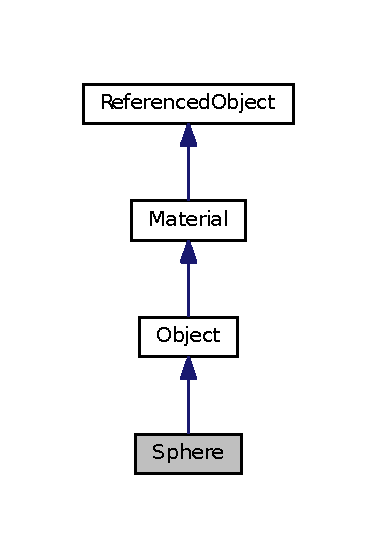
\includegraphics[width=181pt]{class_sphere__inherit__graph}
\end{center}
\end{figure}


Collaboration diagram for Sphere\+:
\nopagebreak
\begin{figure}[H]
\begin{center}
\leavevmode
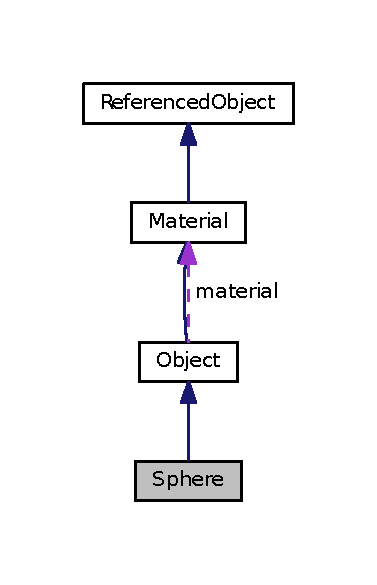
\includegraphics[width=181pt]{class_sphere__coll__graph}
\end{center}
\end{figure}
\subsection*{Public Member Functions}
\begin{DoxyCompactItemize}
\item 
{\bf Sphere} (double {\bf radius})
\item 
{\bf $\sim$\+Sphere} ()
\item 
double {\bf line\+Test} (double origin[3], double direction[3], double max\+Distance)
\begin{DoxyCompactList}\small\item\em Must do the line intersection test and return the closest distance in which a ray originating in origin with given direction intersects the object -\/ if such a point exists closer than max\+Distance. \end{DoxyCompactList}\item 
void {\bf get\+Normal} (double point[3], double normal[3])
\begin{DoxyCompactList}\small\item\em Compute the normal of the object at the given point. \end{DoxyCompactList}\item 
bool {\bf is\+Inside} (double point[3])
\begin{DoxyCompactList}\small\item\em Tests if a point is inside the object or not. \end{DoxyCompactList}\end{DoxyCompactItemize}
\subsection*{Private Attributes}
\begin{DoxyCompactItemize}
\item 
double {\bf radius}
\end{DoxyCompactItemize}
\subsection*{Additional Inherited Members}


\subsection{Detailed Description}
A sphere of given radius. 

Definition at line 33 of file sphere.\+h.



\subsection{Constructor \& Destructor Documentation}
\index{Sphere@{Sphere}!Sphere@{Sphere}}
\index{Sphere@{Sphere}!Sphere@{Sphere}}
\subsubsection[{Sphere}]{\setlength{\rightskip}{0pt plus 5cm}Sphere\+::\+Sphere (
\begin{DoxyParamCaption}
\item[{double}]{radius}
\end{DoxyParamCaption}
)}\label{class_sphere_ad9e68fc78c4e2ccb78098071428155da}


Definition at line 27 of file sphere.\+cc.



References radius.

\index{Sphere@{Sphere}!````~Sphere@{$\sim$\+Sphere}}
\index{````~Sphere@{$\sim$\+Sphere}!Sphere@{Sphere}}
\subsubsection[{$\sim$\+Sphere}]{\setlength{\rightskip}{0pt plus 5cm}Sphere\+::$\sim$\+Sphere (
\begin{DoxyParamCaption}
{}
\end{DoxyParamCaption}
)}\label{class_sphere_a569c071e50a3e11f678630ee1a17737e}


Definition at line 30 of file sphere.\+cc.



\subsection{Member Function Documentation}
\index{Sphere@{Sphere}!get\+Normal@{get\+Normal}}
\index{get\+Normal@{get\+Normal}!Sphere@{Sphere}}
\subsubsection[{get\+Normal}]{\setlength{\rightskip}{0pt plus 5cm}void Sphere\+::get\+Normal (
\begin{DoxyParamCaption}
\item[{double}]{point[3], }
\item[{double}]{normal[3]}
\end{DoxyParamCaption}
)\hspace{0.3cm}{\ttfamily [virtual]}}\label{class_sphere_a36b26e53cef4b521c97df51fac315c68}


Compute the normal of the object at the given point. 

Result is not guaranteed to be of unit length. 

Implements {\bf Object} \doxyref{}{p.}{class_object_a22c15ace5725e2577dbb187265bd3201}.



Definition at line 49 of file sphere.\+cc.



References assign().

\index{Sphere@{Sphere}!is\+Inside@{is\+Inside}}
\index{is\+Inside@{is\+Inside}!Sphere@{Sphere}}
\subsubsection[{is\+Inside}]{\setlength{\rightskip}{0pt plus 5cm}bool Sphere\+::is\+Inside (
\begin{DoxyParamCaption}
\item[{double}]{point[3]}
\end{DoxyParamCaption}
)\hspace{0.3cm}{\ttfamily [virtual]}}\label{class_sphere_a25cf6b133c99f57aa23380c4511507cf}


Tests if a point is inside the object or not. 



Implements {\bf Object} \doxyref{}{p.}{class_object_a652359286747bf237cb2d4d0a802bd18}.



Definition at line 53 of file sphere.\+cc.



References dot\+Product(), and radius.

\index{Sphere@{Sphere}!line\+Test@{line\+Test}}
\index{line\+Test@{line\+Test}!Sphere@{Sphere}}
\subsubsection[{line\+Test}]{\setlength{\rightskip}{0pt plus 5cm}double Sphere\+::line\+Test (
\begin{DoxyParamCaption}
\item[{double}]{origin[3], }
\item[{double}]{direction[3], }
\item[{double}]{max\+Distance}
\end{DoxyParamCaption}
)\hspace{0.3cm}{\ttfamily [virtual]}}\label{class_sphere_a138bf6427c11475d7b42f9debd6a1971}


Must do the line intersection test and return the closest distance in which a ray originating in origin with given direction intersects the object -\/ if such a point exists closer than max\+Distance. 

Returns distance M\+A\+X\+\_\+\+D\+I\+S\+T\+A\+N\+C\+E if no such intersection exists.

Direction is not neccessarily a vector of unit length, and distances are measured in multiples of this vector. 

Implements {\bf Object} \doxyref{}{p.}{class_object_a1bfd7ffbccda28c67d8a537393113a7e}.



Definition at line 32 of file sphere.\+cc.



References dot\+Product(), M\+A\+X\+\_\+\+D\+I\+S\+T\+A\+N\+C\+E, and radius.



\subsection{Member Data Documentation}
\index{Sphere@{Sphere}!radius@{radius}}
\index{radius@{radius}!Sphere@{Sphere}}
\subsubsection[{radius}]{\setlength{\rightskip}{0pt plus 5cm}double Sphere\+::radius\hspace{0.3cm}{\ttfamily [private]}}\label{class_sphere_a45d6c6c870fac7c2a885ad2e226334ad}


Definition at line 43 of file sphere.\+h.



Referenced by is\+Inside(), line\+Test(), and Sphere().



The documentation for this class was generated from the following files\+:\begin{DoxyCompactItemize}
\item 
{\bf sphere.\+h}\item 
{\bf sphere.\+cc}\end{DoxyCompactItemize}

\section{Transform Class Reference}
\label{class_transform}\index{Transform@{Transform}}


Represents generic affine transformations.  




{\ttfamily \#include $<$transform.\+h$>$}



Inheritance diagram for Transform\+:
\nopagebreak
\begin{figure}[H]
\begin{center}
\leavevmode
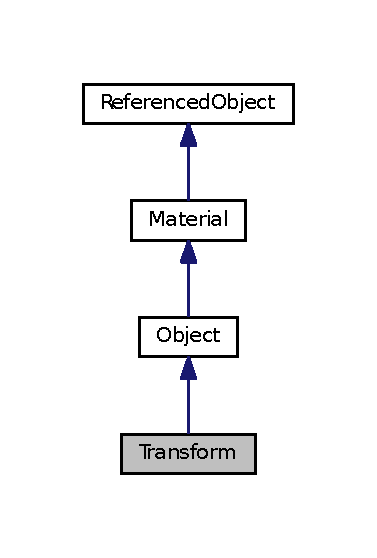
\includegraphics[width=181pt]{class_transform__inherit__graph}
\end{center}
\end{figure}


Collaboration diagram for Transform\+:
\nopagebreak
\begin{figure}[H]
\begin{center}
\leavevmode
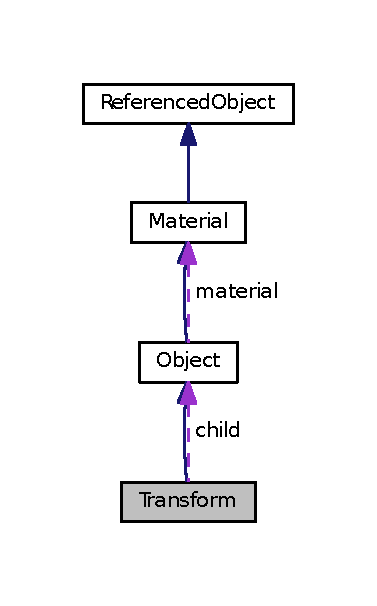
\includegraphics[width=181pt]{class_transform__coll__graph}
\end{center}
\end{figure}
\subsection*{Public Member Functions}
\begin{DoxyCompactItemize}
\item 
{\bf Transform} ({\bf Object} $\ast${\bf child})
\item 
{\bf $\sim$\+Transform} ()
\item 
double {\bf line\+Test} (double origin[3], double direction[3], double max\+Distance)
\begin{DoxyCompactList}\small\item\em Must do the line intersection test and return the closest distance in which a ray originating in origin with given direction intersects the object -\/ if such a point exists closer than max\+Distance. \end{DoxyCompactList}\item 
void {\bf get\+Normal} (double point[3], double normal[3])
\begin{DoxyCompactList}\small\item\em Compute the normal of the object at the given point. \end{DoxyCompactList}\item 
bool {\bf is\+Inside} (double point[3])
\begin{DoxyCompactList}\small\item\em Tests if a point is inside the object or not. \end{DoxyCompactList}\item 
void {\bf identity} ()
\begin{DoxyCompactList}\small\item\em Resets the transform to the identity matrix. \end{DoxyCompactList}\item 
void {\bf translate} (double dx, double dy, double dz)
\begin{DoxyCompactList}\small\item\em Performs a translation. \end{DoxyCompactList}\item 
void {\bf scale} (double sx, double sy, double sz)
\begin{DoxyCompactList}\small\item\em Performs a scale. \end{DoxyCompactList}\item 
void {\bf rotate\+X} (double rad)
\begin{DoxyCompactList}\small\item\em Rotates around X-\/axis. \end{DoxyCompactList}\item 
void {\bf rotate\+Y} (double rad)
\begin{DoxyCompactList}\small\item\em Rotates around Y-\/axis. \end{DoxyCompactList}\item 
void {\bf rotate\+Z} (double rad)
\begin{DoxyCompactList}\small\item\em Rotates around Z-\/axis. \end{DoxyCompactList}\item 
virtual void {\bf get\+Lighting\+Properties} (double point[3], {\bf Lighting\+Properties} $\ast$props, double normal[3])
\begin{DoxyCompactList}\small\item\em Default material handling that queries the default material given for this object. \end{DoxyCompactList}\end{DoxyCompactItemize}
\subsection*{Private Member Functions}
\begin{DoxyCompactItemize}
\item 
void {\bf compute\+Inverse\+Transform} ()
\end{DoxyCompactItemize}
\subsection*{Private Attributes}
\begin{DoxyCompactItemize}
\item 
{\bf Matrix4d} {\bf forward}
\item 
{\bf Matrix4d} {\bf inverse}
\item 
{\bf Object} $\ast$ {\bf child}
\end{DoxyCompactItemize}
\subsection*{Additional Inherited Members}


\subsection{Detailed Description}
Represents generic affine transformations. 

Can contain a single child object and performs a transformation on it's position and shape. 

Definition at line 35 of file transform.\+h.



\subsection{Constructor \& Destructor Documentation}
\index{Transform@{Transform}!Transform@{Transform}}
\index{Transform@{Transform}!Transform@{Transform}}
\subsubsection[{Transform}]{\setlength{\rightskip}{0pt plus 5cm}Transform\+::\+Transform (
\begin{DoxyParamCaption}
\item[{{\bf Object} $\ast$}]{child}
\end{DoxyParamCaption}
)}\label{class_transform_acb364a599881f5af97c2ce69afeab9e3}


Definition at line 27 of file transform.\+cc.



References child, forward, identity\+Matrix(), inverse, and Referenced\+Object\+::reference().

\index{Transform@{Transform}!````~Transform@{$\sim$\+Transform}}
\index{````~Transform@{$\sim$\+Transform}!Transform@{Transform}}
\subsubsection[{$\sim$\+Transform}]{\setlength{\rightskip}{0pt plus 5cm}Transform\+::$\sim$\+Transform (
\begin{DoxyParamCaption}
{}
\end{DoxyParamCaption}
)}\label{class_transform_aa72e286c069850db80927b0e6554cd3e}


Definition at line 33 of file transform.\+cc.



References child, and Referenced\+Object\+::dereference().



\subsection{Member Function Documentation}
\index{Transform@{Transform}!compute\+Inverse\+Transform@{compute\+Inverse\+Transform}}
\index{compute\+Inverse\+Transform@{compute\+Inverse\+Transform}!Transform@{Transform}}
\subsubsection[{compute\+Inverse\+Transform}]{\setlength{\rightskip}{0pt plus 5cm}void Transform\+::compute\+Inverse\+Transform (
\begin{DoxyParamCaption}
{}
\end{DoxyParamCaption}
)\hspace{0.3cm}{\ttfamily [private]}}\label{class_transform_a35e1780391bceb62e9be789b835c0167}


Definition at line 121 of file transform.\+cc.



References forward, and inverse.



Referenced by rotate\+X(), rotate\+Y(), rotate\+Z(), scale(), and translate().

\index{Transform@{Transform}!get\+Lighting\+Properties@{get\+Lighting\+Properties}}
\index{get\+Lighting\+Properties@{get\+Lighting\+Properties}!Transform@{Transform}}
\subsubsection[{get\+Lighting\+Properties}]{\setlength{\rightskip}{0pt plus 5cm}void Transform\+::get\+Lighting\+Properties (
\begin{DoxyParamCaption}
\item[{double}]{point[3], }
\item[{{\bf Lighting\+Properties} $\ast$}]{props, }
\item[{double}]{normal[3]}
\end{DoxyParamCaption}
)\hspace{0.3cm}{\ttfamily [virtual]}}\label{class_transform_a6759fe52b87d9113c48c0414824ac067}


Default material handling that queries the default material given for this object. 



Reimplemented from {\bf Object} \doxyref{}{p.}{class_object_a510171215bdf364cc0bf8f72336039b9}.



Definition at line 159 of file transform.\+cc.



References child, Material\+::get\+Lighting\+Properties(), Object\+::get\+Lighting\+Properties(), inverse, and Object\+::material.

\index{Transform@{Transform}!get\+Normal@{get\+Normal}}
\index{get\+Normal@{get\+Normal}!Transform@{Transform}}
\subsubsection[{get\+Normal}]{\setlength{\rightskip}{0pt plus 5cm}void Transform\+::get\+Normal (
\begin{DoxyParamCaption}
\item[{double}]{point[3], }
\item[{double}]{normal[3]}
\end{DoxyParamCaption}
)\hspace{0.3cm}{\ttfamily [virtual]}}\label{class_transform_ab9b4a86bde00d015be3ee563a072ceeb}


Compute the normal of the object at the given point. 

Result is not guaranteed to be of unit length. 

Implements {\bf Object} \doxyref{}{p.}{class_object_a22c15ace5725e2577dbb187265bd3201}.



Definition at line 57 of file transform.\+cc.



References assign(), child, forward, Object\+::get\+Normal(), and inverse.

\index{Transform@{Transform}!identity@{identity}}
\index{identity@{identity}!Transform@{Transform}}
\subsubsection[{identity}]{\setlength{\rightskip}{0pt plus 5cm}void Transform\+::identity (
\begin{DoxyParamCaption}
{}
\end{DoxyParamCaption}
)}\label{class_transform_a9122d9edc46ba725896912e0b1ac6415}


Resets the transform to the identity matrix. 



Definition at line 81 of file transform.\+cc.



References forward, identity\+Matrix(), and inverse.



Referenced by do\+Redraw().

\index{Transform@{Transform}!is\+Inside@{is\+Inside}}
\index{is\+Inside@{is\+Inside}!Transform@{Transform}}
\subsubsection[{is\+Inside}]{\setlength{\rightskip}{0pt plus 5cm}bool Transform\+::is\+Inside (
\begin{DoxyParamCaption}
\item[{double}]{point[3]}
\end{DoxyParamCaption}
)\hspace{0.3cm}{\ttfamily [virtual]}}\label{class_transform_acf224e03c58e2923df817808f66f1cd0}


Tests if a point is inside the object or not. 



Implements {\bf Object} \doxyref{}{p.}{class_object_a652359286747bf237cb2d4d0a802bd18}.



Definition at line 71 of file transform.\+cc.



References child, inverse, and Object\+::is\+Inside().

\index{Transform@{Transform}!line\+Test@{line\+Test}}
\index{line\+Test@{line\+Test}!Transform@{Transform}}
\subsubsection[{line\+Test}]{\setlength{\rightskip}{0pt plus 5cm}double Transform\+::line\+Test (
\begin{DoxyParamCaption}
\item[{double}]{origin[3], }
\item[{double}]{direction[3], }
\item[{double}]{max\+Distance}
\end{DoxyParamCaption}
)\hspace{0.3cm}{\ttfamily [virtual]}}\label{class_transform_ab2e6df43a4e87522a6e446b10cd67ca5}


Must do the line intersection test and return the closest distance in which a ray originating in origin with given direction intersects the object -\/ if such a point exists closer than max\+Distance. 

Returns distance M\+A\+X\+\_\+\+D\+I\+S\+T\+A\+N\+C\+E if no such intersection exists.

Direction is not neccessarily a vector of unit length, and distances are measured in multiples of this vector. 

Implements {\bf Object} \doxyref{}{p.}{class_object_a1bfd7ffbccda28c67d8a537393113a7e}.



Definition at line 36 of file transform.\+cc.



References child, inverse, and Object\+::line\+Test().

\index{Transform@{Transform}!rotate\+X@{rotate\+X}}
\index{rotate\+X@{rotate\+X}!Transform@{Transform}}
\subsubsection[{rotate\+X}]{\setlength{\rightskip}{0pt plus 5cm}void Transform\+::rotate\+X (
\begin{DoxyParamCaption}
\item[{double}]{rad}
\end{DoxyParamCaption}
)}\label{class_transform_a7ecb04da3bdd25a299452f69e302512f}


Rotates around X-\/axis. 



Definition at line 107 of file transform.\+cc.



References compute\+Inverse\+Transform(), forward, and rotate\+Matrix\+X().



Referenced by do\+Redraw().

\index{Transform@{Transform}!rotate\+Y@{rotate\+Y}}
\index{rotate\+Y@{rotate\+Y}!Transform@{Transform}}
\subsubsection[{rotate\+Y}]{\setlength{\rightskip}{0pt plus 5cm}void Transform\+::rotate\+Y (
\begin{DoxyParamCaption}
\item[{double}]{rad}
\end{DoxyParamCaption}
)}\label{class_transform_ac54a047451961ed8e8268c872c3d7855}


Rotates around Y-\/axis. 



Definition at line 111 of file transform.\+cc.



References compute\+Inverse\+Transform(), forward, and rotate\+Matrix\+Y().

\index{Transform@{Transform}!rotate\+Z@{rotate\+Z}}
\index{rotate\+Z@{rotate\+Z}!Transform@{Transform}}
\subsubsection[{rotate\+Z}]{\setlength{\rightskip}{0pt plus 5cm}void Transform\+::rotate\+Z (
\begin{DoxyParamCaption}
\item[{double}]{rad}
\end{DoxyParamCaption}
)}\label{class_transform_a370bac8b5f52e188a4f5ec06e245c1d0}


Rotates around Z-\/axis. 



Definition at line 115 of file transform.\+cc.



References compute\+Inverse\+Transform(), forward, and rotate\+Matrix\+Z().

\index{Transform@{Transform}!scale@{scale}}
\index{scale@{scale}!Transform@{Transform}}
\subsubsection[{scale}]{\setlength{\rightskip}{0pt plus 5cm}void Transform\+::scale (
\begin{DoxyParamCaption}
\item[{double}]{sx, }
\item[{double}]{sy, }
\item[{double}]{sz}
\end{DoxyParamCaption}
)}\label{class_transform_addd574de402c013667da89d92b443bc5}


Performs a scale. 



Definition at line 97 of file transform.\+cc.



References assign(), compute\+Inverse\+Transform(), forward, identity\+Matrix(), and matrix\+Mult().



Referenced by do\+Redraw().

\index{Transform@{Transform}!translate@{translate}}
\index{translate@{translate}!Transform@{Transform}}
\subsubsection[{translate}]{\setlength{\rightskip}{0pt plus 5cm}void Transform\+::translate (
\begin{DoxyParamCaption}
\item[{double}]{dx, }
\item[{double}]{dy, }
\item[{double}]{dz}
\end{DoxyParamCaption}
)}\label{class_transform_a141efd4815b5781e066bdce4c17ea84e}


Performs a translation. 



Definition at line 86 of file transform.\+cc.



References assign(), compute\+Inverse\+Transform(), forward, identity\+Matrix(), and matrix\+Mult().



Referenced by do\+Redraw().



\subsection{Member Data Documentation}
\index{Transform@{Transform}!child@{child}}
\index{child@{child}!Transform@{Transform}}
\subsubsection[{child}]{\setlength{\rightskip}{0pt plus 5cm}{\bf Object}$\ast$ Transform\+::child\hspace{0.3cm}{\ttfamily [private]}}\label{class_transform_a9e59d97ee1e2e57aac99e54b701aaa7f}


Definition at line 68 of file transform.\+h.



Referenced by get\+Lighting\+Properties(), get\+Normal(), is\+Inside(), line\+Test(), Transform(), and $\sim$\+Transform().

\index{Transform@{Transform}!forward@{forward}}
\index{forward@{forward}!Transform@{Transform}}
\subsubsection[{forward}]{\setlength{\rightskip}{0pt plus 5cm}{\bf Matrix4d} Transform\+::forward\hspace{0.3cm}{\ttfamily [private]}}\label{class_transform_a6e65bb3381497a182ce6cc5e4f6fff81}


Definition at line 66 of file transform.\+h.



Referenced by compute\+Inverse\+Transform(), get\+Normal(), identity(), rotate\+X(), rotate\+Y(), rotate\+Z(), scale(), Transform(), and translate().

\index{Transform@{Transform}!inverse@{inverse}}
\index{inverse@{inverse}!Transform@{Transform}}
\subsubsection[{inverse}]{\setlength{\rightskip}{0pt plus 5cm}{\bf Matrix4d} Transform\+::inverse\hspace{0.3cm}{\ttfamily [private]}}\label{class_transform_a8d4b9aaaea2fb541ea45c334f9caa537}


Definition at line 67 of file transform.\+h.



Referenced by compute\+Inverse\+Transform(), get\+Lighting\+Properties(), get\+Normal(), identity(), is\+Inside(), line\+Test(), and Transform().



The documentation for this class was generated from the following files\+:\begin{DoxyCompactItemize}
\item 
{\bf transform.\+h}\item 
{\bf transform.\+cc}\end{DoxyCompactItemize}

\chapter{File Documentation}
\section{camera.\+cc File Reference}
\label{camera_8cc}\index{camera.\+cc@{camera.\+cc}}


Implements all methods for the \doxyref{Camera}{p.}{class_camera} class.  


{\ttfamily \#include \char`\"{}general.\+h\char`\"{}}\\*
{\ttfamily \#include \char`\"{}camera.\+h\char`\"{}}\\*
Include dependency graph for camera.\+cc\+:
\nopagebreak
\begin{figure}[H]
\begin{center}
\leavevmode
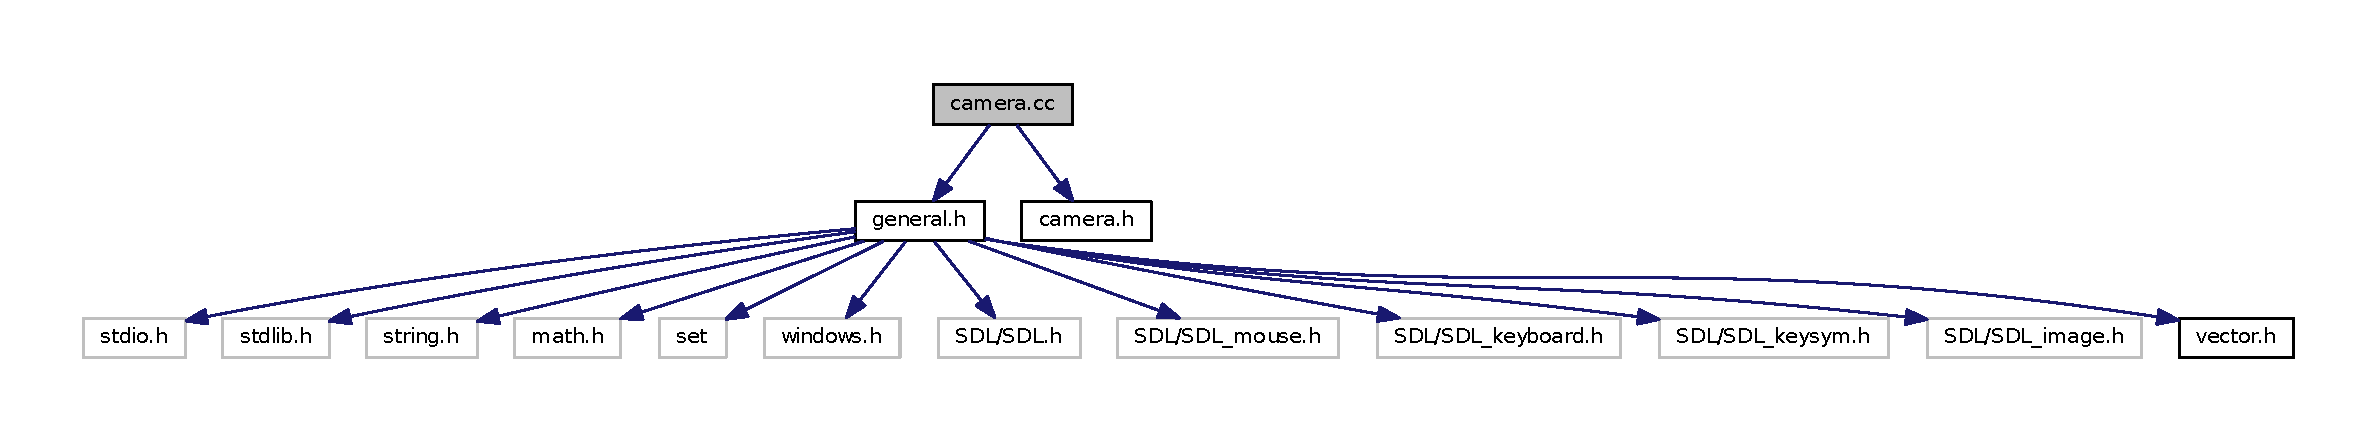
\includegraphics[width=350pt]{camera_8cc__incl}
\end{center}
\end{figure}


\subsection{Detailed Description}
Implements all methods for the \doxyref{Camera}{p.}{class_camera} class. 



Definition in file {\bf camera.\+cc}.


\section{camera.\+h File Reference}
\label{camera_8h}\index{camera.\+h@{camera.\+h}}


Declares all methods for the \doxyref{Camera}{p.}{class_camera} class.  


This graph shows which files directly or indirectly include this file\+:
\nopagebreak
\begin{figure}[H]
\begin{center}
\leavevmode
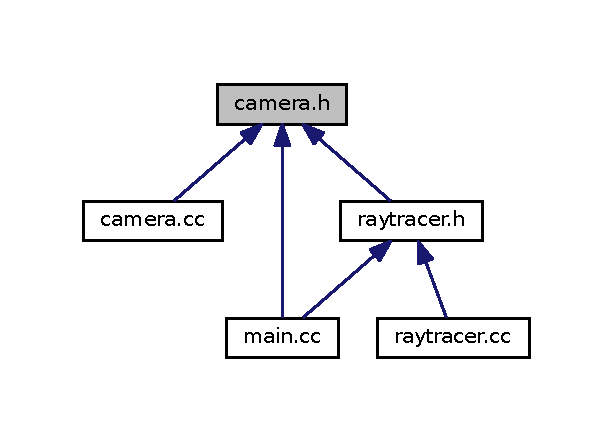
\includegraphics[width=294pt]{camera_8h__dep__incl}
\end{center}
\end{figure}
\subsection*{Classes}
\begin{DoxyCompactItemize}
\item 
class {\bf Camera}
\begin{DoxyCompactList}\small\item\em Represents the camera and determines the point from which rays are cast in the scene. \end{DoxyCompactList}\end{DoxyCompactItemize}


\subsection{Detailed Description}
Declares all methods for the \doxyref{Camera}{p.}{class_camera} class. 



Definition in file {\bf camera.\+h}.


\section{csg.\+cc File Reference}
\label{csg_8cc}\index{csg.\+cc@{csg.\+cc}}


Implements all methods for all C\+S\+G classes (\doxyref{Intersection}{p.}{class_intersection}, \doxyref{Inverse}{p.}{class_inverse})  


{\ttfamily \#include \char`\"{}general.\+h\char`\"{}}\\*
{\ttfamily \#include \char`\"{}csg.\+h\char`\"{}}\\*
{\ttfamily \#include $<$omp.\+h$>$}\\*
Include dependency graph for csg.\+cc\+:
\nopagebreak
\begin{figure}[H]
\begin{center}
\leavevmode
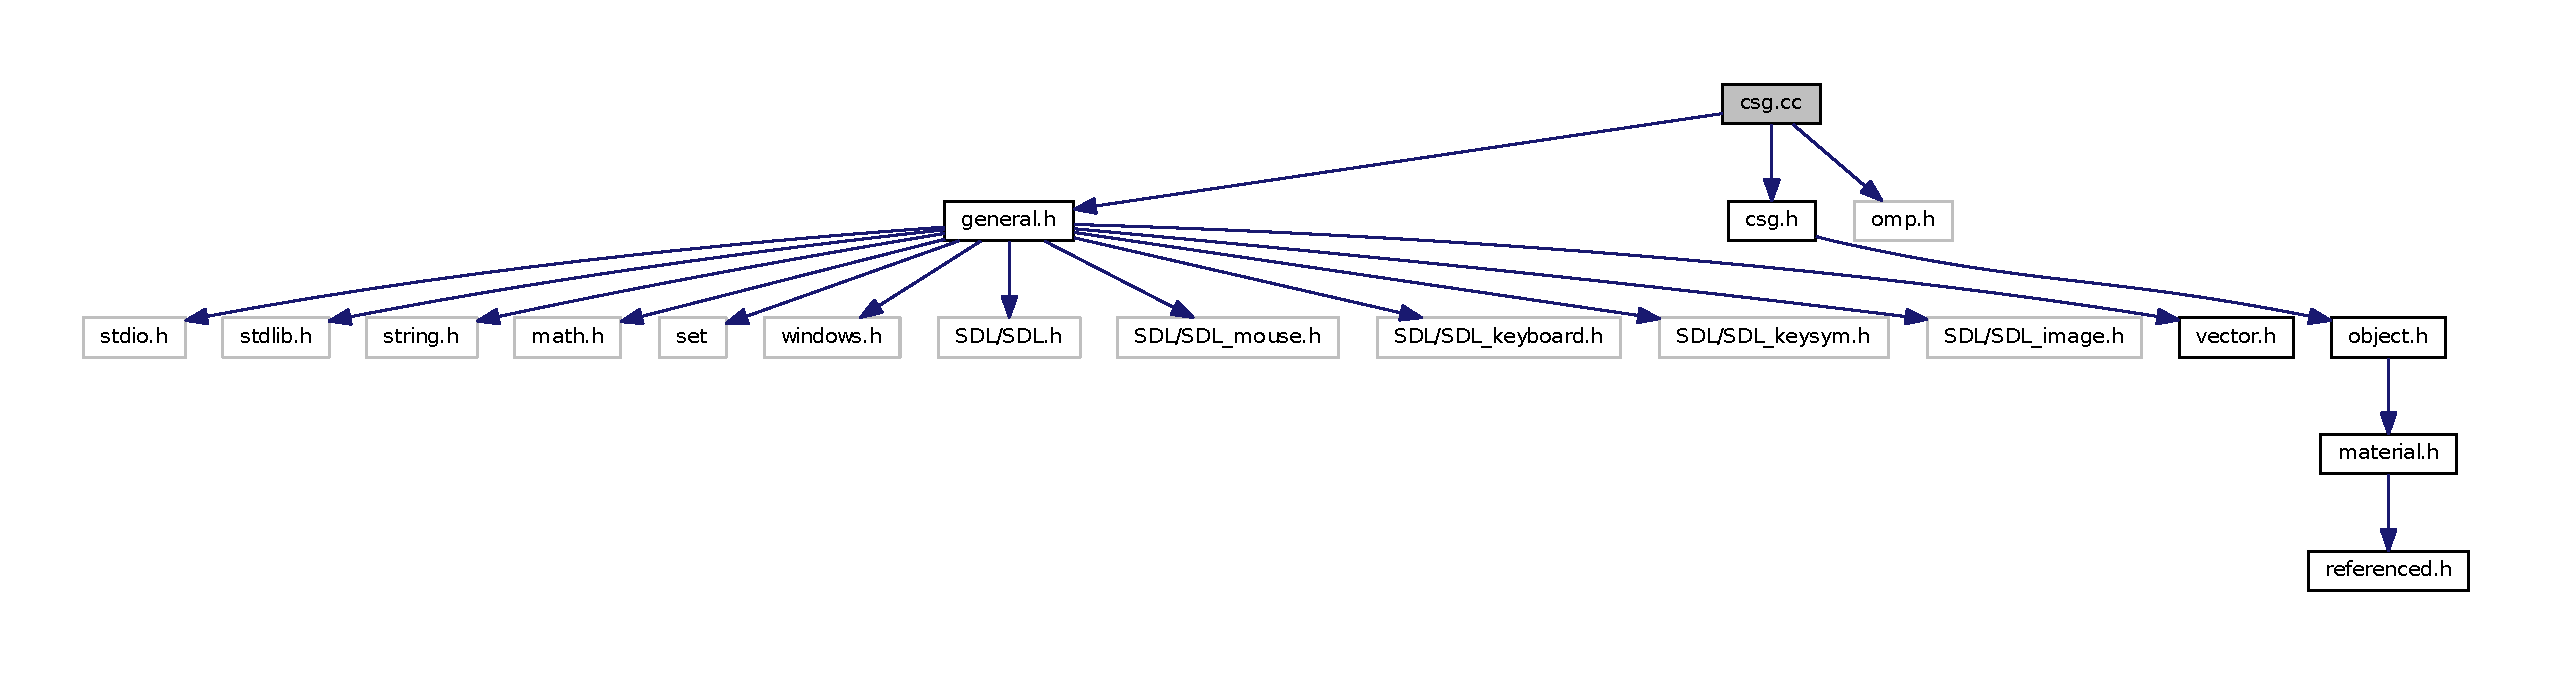
\includegraphics[width=350pt]{csg_8cc__incl}
\end{center}
\end{figure}


\subsection{Detailed Description}
Implements all methods for all C\+S\+G classes (\doxyref{Intersection}{p.}{class_intersection}, \doxyref{Inverse}{p.}{class_inverse}) 



Definition in file {\bf csg.\+cc}.


\section{csg.\+h File Reference}
\label{csg_8h}\index{csg.\+h@{csg.\+h}}


Declares all methods for all C\+S\+G classes (\doxyref{Intersection}{p.}{class_intersection}, \doxyref{Inverse}{p.}{class_inverse})  


{\ttfamily \#include \char`\"{}object.\+h\char`\"{}}\\*
Include dependency graph for csg.\+h\+:
\nopagebreak
\begin{figure}[H]
\begin{center}
\leavevmode
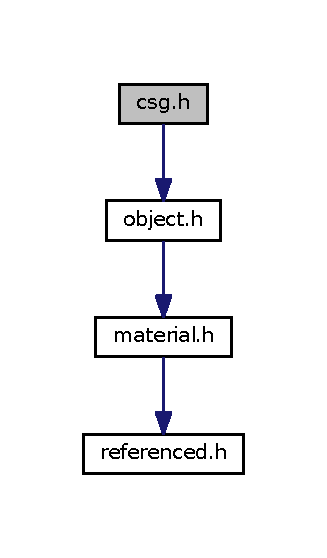
\includegraphics[width=157pt]{csg_8h__incl}
\end{center}
\end{figure}
This graph shows which files directly or indirectly include this file\+:
\nopagebreak
\begin{figure}[H]
\begin{center}
\leavevmode
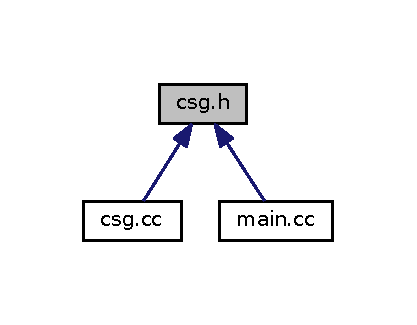
\includegraphics[width=200pt]{csg_8h__dep__incl}
\end{center}
\end{figure}
\subsection*{Classes}
\begin{DoxyCompactItemize}
\item 
class {\bf Intersection}
\begin{DoxyCompactList}\small\item\em Creates new objects as the intersection of multiple child objects. \end{DoxyCompactList}\item 
class {\bf Inverse}
\begin{DoxyCompactList}\small\item\em Creates the inverse of an object by negating the \doxyref{Object\+::is\+Inside}{p.}{class_object_a652359286747bf237cb2d4d0a802bd18} and Object\+::\+Get\+Normal functions. \end{DoxyCompactList}\end{DoxyCompactItemize}


\subsection{Detailed Description}
Declares all methods for all C\+S\+G classes (\doxyref{Intersection}{p.}{class_intersection}, \doxyref{Inverse}{p.}{class_inverse}) 



Definition in file {\bf csg.\+h}.


\section{general.\+h File Reference}
\label{general_8h}\index{general.\+h@{general.\+h}}


Contains common type definitions, includes, etc.  


{\ttfamily \#include $<$stdio.\+h$>$}\\*
{\ttfamily \#include $<$stdlib.\+h$>$}\\*
{\ttfamily \#include $<$string.\+h$>$}\\*
{\ttfamily \#include $<$math.\+h$>$}\\*
{\ttfamily \#include $<$set$>$}\\*
{\ttfamily \#include $<$windows.\+h$>$}\\*
{\ttfamily \#include \char`\"{}S\+D\+L/\+S\+D\+L.\+h\char`\"{}}\\*
{\ttfamily \#include \char`\"{}S\+D\+L/\+S\+D\+L\+\_\+mouse.\+h\char`\"{}}\\*
{\ttfamily \#include \char`\"{}S\+D\+L/\+S\+D\+L\+\_\+keyboard.\+h\char`\"{}}\\*
{\ttfamily \#include \char`\"{}S\+D\+L/\+S\+D\+L\+\_\+keysym.\+h\char`\"{}}\\*
{\ttfamily \#include \char`\"{}S\+D\+L/\+S\+D\+L\+\_\+image.\+h\char`\"{}}\\*
{\ttfamily \#include \char`\"{}vector.\+h\char`\"{}}\\*
Include dependency graph for general.\+h\+:
\nopagebreak
\begin{figure}[H]
\begin{center}
\leavevmode
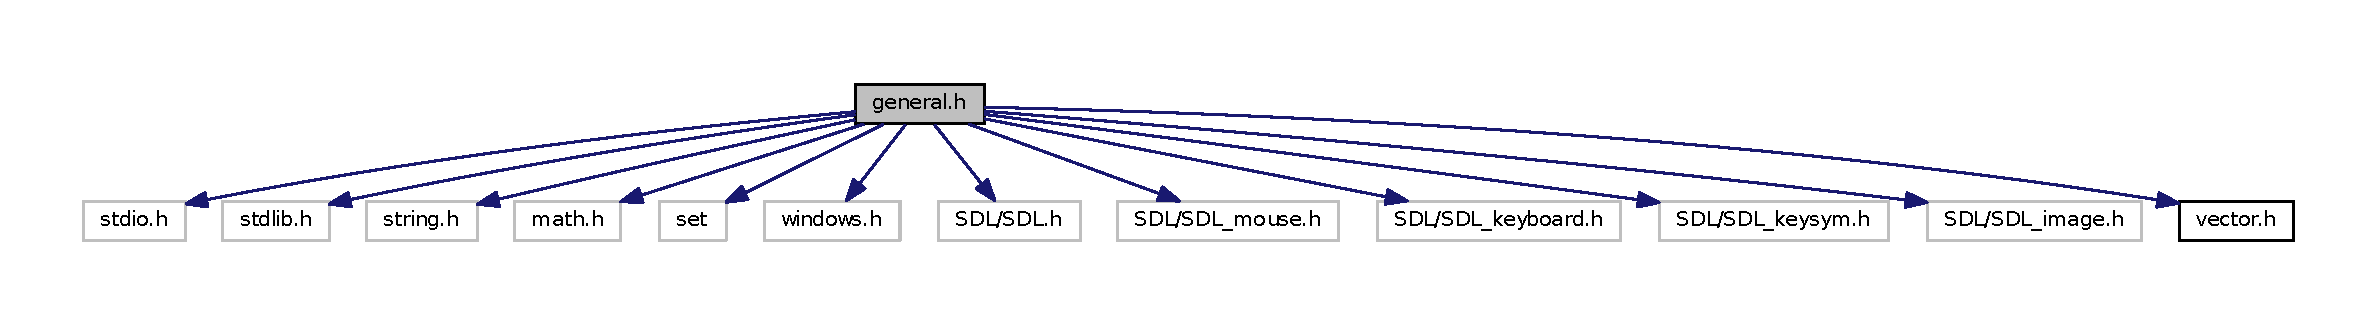
\includegraphics[width=350pt]{general_8h__incl}
\end{center}
\end{figure}
This graph shows which files directly or indirectly include this file\+:
\nopagebreak
\begin{figure}[H]
\begin{center}
\leavevmode
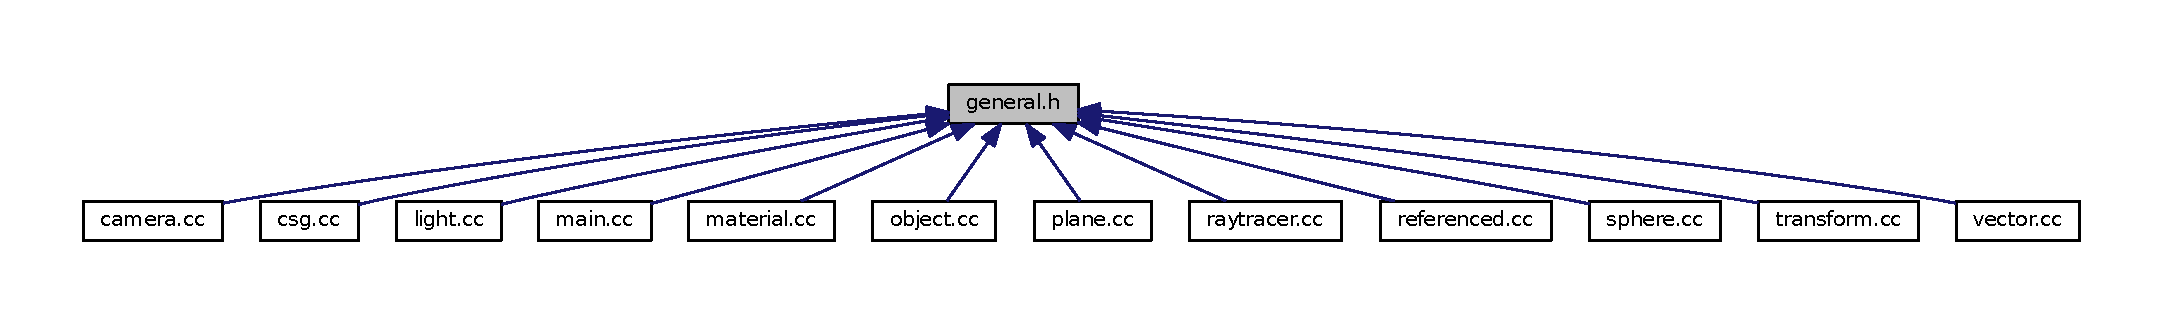
\includegraphics[width=350pt]{general_8h__dep__incl}
\end{center}
\end{figure}
\subsection*{Macros}
\begin{DoxyCompactItemize}
\item 
\#define {\bf M\+I\+N}(x, y)~((x)$<$(y)?(x)\+:(y))
\item 
\#define {\bf M\+A\+X}(x, y)~((x)$>$(y)?(x)\+:(y))
\item 
\#define {\bf M\+\_\+\+P\+I}~3.\+14159265
\item 
\#define {\bf M\+A\+X\+\_\+\+O\+M\+P\+\_\+\+T\+H\+R\+E\+A\+D\+S}~32
\end{DoxyCompactItemize}
\subsection*{Functions}
\begin{DoxyCompactItemize}
\item 
void {\bf print\+Debug\+Indentation} ()
\end{DoxyCompactItemize}
\subsection*{Variables}
\begin{DoxyCompactItemize}
\item 
int {\bf debug\+This\+Pixel}
\item 
int {\bf debug\+Indentation}
\end{DoxyCompactItemize}


\subsection{Detailed Description}
Contains common type definitions, includes, etc. 

for all labs 

Definition in file {\bf general.\+h}.



\subsection{Macro Definition Documentation}
\index{general.\+h@{general.\+h}!M\+\_\+\+P\+I@{M\+\_\+\+P\+I}}
\index{M\+\_\+\+P\+I@{M\+\_\+\+P\+I}!general.\+h@{general.\+h}}
\subsubsection[{M\+\_\+\+P\+I}]{\setlength{\rightskip}{0pt plus 5cm}\#define M\+\_\+\+P\+I~3.\+14159265}\label{general_8h_ae71449b1cc6e6250b91f539153a7a0d3}


Definition at line 51 of file general.\+h.



Referenced by do\+Redraw().

\index{general.\+h@{general.\+h}!M\+A\+X@{M\+A\+X}}
\index{M\+A\+X@{M\+A\+X}!general.\+h@{general.\+h}}
\subsubsection[{M\+A\+X}]{\setlength{\rightskip}{0pt plus 5cm}\#define M\+A\+X(
\begin{DoxyParamCaption}
\item[{}]{x, }
\item[{}]{y}
\end{DoxyParamCaption}
)~((x)$>$(y)?(x)\+:(y))}\label{general_8h_aacc3ee1a7f283f8ef65cea31f4436a95}


Definition at line 48 of file general.\+h.

\index{general.\+h@{general.\+h}!M\+A\+X\+\_\+\+O\+M\+P\+\_\+\+T\+H\+R\+E\+A\+D\+S@{M\+A\+X\+\_\+\+O\+M\+P\+\_\+\+T\+H\+R\+E\+A\+D\+S}}
\index{M\+A\+X\+\_\+\+O\+M\+P\+\_\+\+T\+H\+R\+E\+A\+D\+S@{M\+A\+X\+\_\+\+O\+M\+P\+\_\+\+T\+H\+R\+E\+A\+D\+S}!general.\+h@{general.\+h}}
\subsubsection[{M\+A\+X\+\_\+\+O\+M\+P\+\_\+\+T\+H\+R\+E\+A\+D\+S}]{\setlength{\rightskip}{0pt plus 5cm}\#define M\+A\+X\+\_\+\+O\+M\+P\+\_\+\+T\+H\+R\+E\+A\+D\+S~32}\label{general_8h_a44940083ba78c21d097d37dcc0a49aec}


Definition at line 57 of file general.\+h.



Referenced by Intersection\+::\+Intersection().

\index{general.\+h@{general.\+h}!M\+I\+N@{M\+I\+N}}
\index{M\+I\+N@{M\+I\+N}!general.\+h@{general.\+h}}
\subsubsection[{M\+I\+N}]{\setlength{\rightskip}{0pt plus 5cm}\#define M\+I\+N(
\begin{DoxyParamCaption}
\item[{}]{x, }
\item[{}]{y}
\end{DoxyParamCaption}
)~((x)$<$(y)?(x)\+:(y))}\label{general_8h_a74e75242132eaabbc1c512488a135926}


Definition at line 47 of file general.\+h.



\subsection{Function Documentation}
\index{general.\+h@{general.\+h}!print\+Debug\+Indentation@{print\+Debug\+Indentation}}
\index{print\+Debug\+Indentation@{print\+Debug\+Indentation}!general.\+h@{general.\+h}}
\subsubsection[{print\+Debug\+Indentation}]{\setlength{\rightskip}{0pt plus 5cm}void print\+Debug\+Indentation (
\begin{DoxyParamCaption}
{}
\end{DoxyParamCaption}
)}\label{general_8h_ae1c327e9afb4e6ccd35029355384fe71}


Definition at line 291 of file main.\+cc.



References debug\+Indentation.



Referenced by Plane\+::line\+Test(), Intersection\+::line\+Test(), and Raytracer\+::raytrace().



\subsection{Variable Documentation}
\index{general.\+h@{general.\+h}!debug\+Indentation@{debug\+Indentation}}
\index{debug\+Indentation@{debug\+Indentation}!general.\+h@{general.\+h}}
\subsubsection[{debug\+Indentation}]{\setlength{\rightskip}{0pt plus 5cm}int debug\+Indentation}\label{general_8h_a5906e7ce057ac03baa7e87832fcad510}


Definition at line 84 of file main.\+cc.



Referenced by Intersection\+::line\+Test(), print\+Debug\+Indentation(), and Raytracer\+::raytrace().

\index{general.\+h@{general.\+h}!debug\+This\+Pixel@{debug\+This\+Pixel}}
\index{debug\+This\+Pixel@{debug\+This\+Pixel}!general.\+h@{general.\+h}}
\subsubsection[{debug\+This\+Pixel}]{\setlength{\rightskip}{0pt plus 5cm}int debug\+This\+Pixel}\label{general_8h_a030f3c150bfe06af45f51ded93eb4d57}


Definition at line 83 of file main.\+cc.



Referenced by do\+Redraw(), Plane\+::line\+Test(), Intersection\+::line\+Test(), and Raytracer\+::raytrace().


\section{light.\+cc File Reference}
\label{light_8cc}\index{light.\+cc@{light.\+cc}}


Implements all methods for the \doxyref{Light}{p.}{class_light} class.  


{\ttfamily \#include \char`\"{}general.\+h\char`\"{}}\\*
{\ttfamily \#include \char`\"{}light.\+h\char`\"{}}\\*
Include dependency graph for light.\+cc\+:
\nopagebreak
\begin{figure}[H]
\begin{center}
\leavevmode
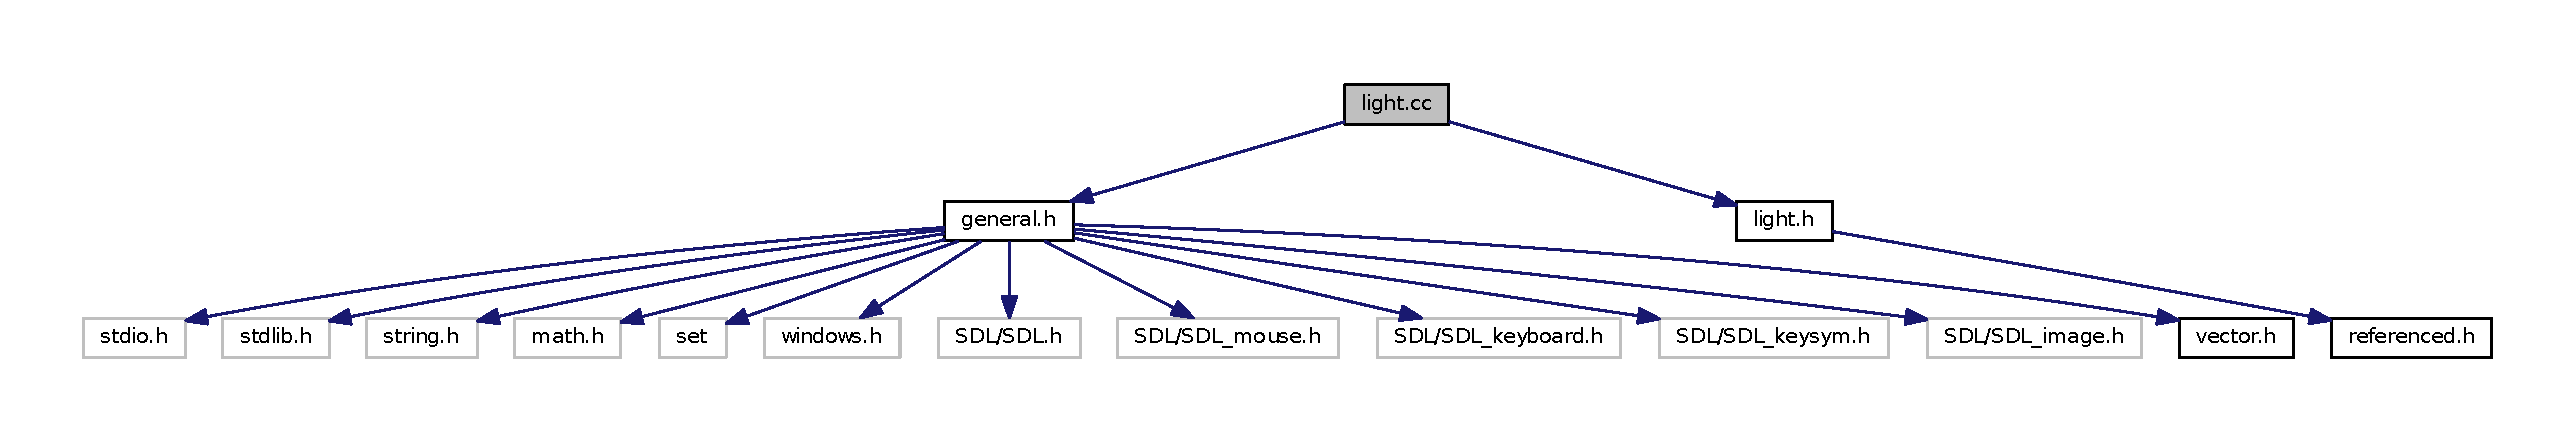
\includegraphics[width=350pt]{light_8cc__incl}
\end{center}
\end{figure}


\subsection{Detailed Description}
Implements all methods for the \doxyref{Light}{p.}{class_light} class. 



Definition in file {\bf light.\+cc}.


\section{light.\+h File Reference}
\label{light_8h}\index{light.\+h@{light.\+h}}


Declares all methods for the \doxyref{Light}{p.}{class_light} class.  


{\ttfamily \#include \char`\"{}referenced.\+h\char`\"{}}\\*
Include dependency graph for light.\+h\+:
\nopagebreak
\begin{figure}[H]
\begin{center}
\leavevmode
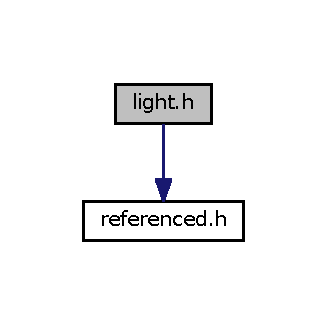
\includegraphics[width=157pt]{light_8h__incl}
\end{center}
\end{figure}
This graph shows which files directly or indirectly include this file\+:
\nopagebreak
\begin{figure}[H]
\begin{center}
\leavevmode
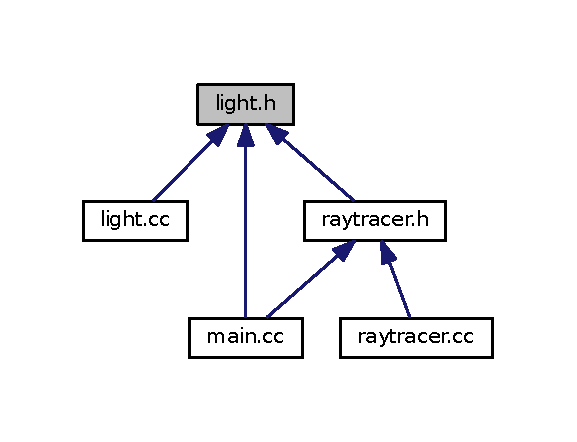
\includegraphics[width=277pt]{light_8h__dep__incl}
\end{center}
\end{figure}
\subsection*{Classes}
\begin{DoxyCompactItemize}
\item 
class {\bf Light}
\begin{DoxyCompactList}\small\item\em Represents a simple direct point light in the scene. \end{DoxyCompactList}\end{DoxyCompactItemize}


\subsection{Detailed Description}
Declares all methods for the \doxyref{Light}{p.}{class_light} class. 



Definition in file {\bf light.\+h}.


\section{main.\+cc File Reference}
\label{main_8cc}\index{main.\+cc@{main.\+cc}}


The main entry point and code skeleton for a raytracer.  


{\ttfamily \#include \char`\"{}general.\+h\char`\"{}}\\*
{\ttfamily \#include \char`\"{}camera.\+h\char`\"{}}\\*
{\ttfamily \#include \char`\"{}raytracer.\+h\char`\"{}}\\*
{\ttfamily \#include \char`\"{}sphere.\+h\char`\"{}}\\*
{\ttfamily \#include \char`\"{}plane.\+h\char`\"{}}\\*
{\ttfamily \#include \char`\"{}light.\+h\char`\"{}}\\*
{\ttfamily \#include \char`\"{}transform.\+h\char`\"{}}\\*
{\ttfamily \#include \char`\"{}noise.\+h\char`\"{}}\\*
{\ttfamily \#include \char`\"{}csg.\+h\char`\"{}}\\*
Include dependency graph for main.\+cc\+:
\nopagebreak
\begin{figure}[H]
\begin{center}
\leavevmode
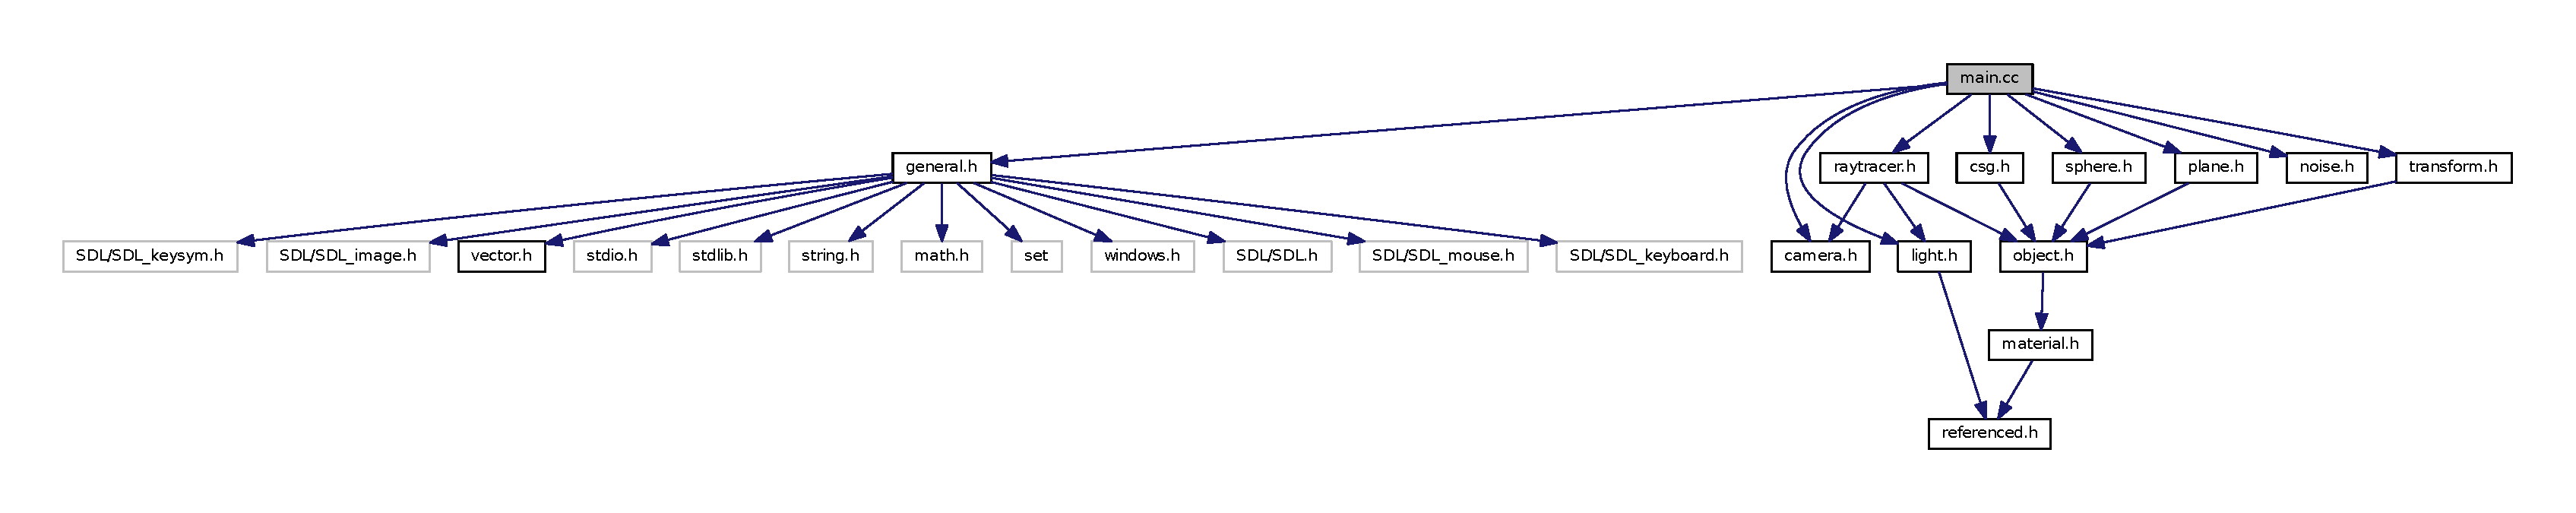
\includegraphics[width=350pt]{main_8cc__incl}
\end{center}
\end{figure}
\subsection*{Functions}
\begin{DoxyCompactItemize}
\item 
void {\bf do\+Redraw} ()
\item 
void {\bf do\+Keyboard} (int, int, int)
\item 
void {\bf tick} (double)
\item 
void $\ast$ {\bf rendering\+Thread} (void $\ast$arg)
\item 
void {\bf render\+Pixels} (int offset, int skip)
\item 
int {\bf main} (int argc, char $\ast$$\ast$args)
\item 
void {\bf put\+Pixel} (int x, int y, int r, int g, int b)
\item 
void {\bf print\+Debug\+Indentation} ()
\end{DoxyCompactItemize}
\subsection*{Variables}
\begin{DoxyCompactItemize}
\item 
int {\bf screen\+Width}
\item 
int {\bf screen\+Height}
\item 
int {\bf is\+Running}
\item 
double {\bf g\+Time}
\item 
double {\bf simulation\+Speed} =5.\+0
\item 
S\+D\+L\+\_\+\+Surface $\ast$ {\bf screen}
\item 
double {\bf camera\+Orbit} [2] =\{0.\+0,0.\+0\}
\item 
{\bf Raytracer} $\ast$ {\bf raytracer}
\item 
{\bf Transform} $\ast$ {\bf object1}
\item 
{\bf Transform} $\ast$ {\bf object2}
\item 
int {\bf debug\+Pixel\+X} =-\/1
\begin{DoxyCompactList}\small\item\em Used for debugging, note that we drop down to singel threaded mode when we are using this per-\/pixel debugging. \end{DoxyCompactList}\item 
int {\bf debug\+Pixel\+Y}
\item 
int {\bf debug\+This\+Pixel} =0
\item 
int {\bf debug\+Indentation} =0
\end{DoxyCompactItemize}


\subsection{Detailed Description}
The main entry point and code skeleton for a raytracer. 



Definition in file {\bf main.\+cc}.



\subsection{Function Documentation}
\index{main.\+cc@{main.\+cc}!do\+Keyboard@{do\+Keyboard}}
\index{do\+Keyboard@{do\+Keyboard}!main.\+cc@{main.\+cc}}
\subsubsection[{do\+Keyboard}]{\setlength{\rightskip}{0pt plus 5cm}void do\+Keyboard (
\begin{DoxyParamCaption}
\item[{int}]{key, }
\item[{int}]{mouse\+X, }
\item[{int}]{mouse\+Y}
\end{DoxyParamCaption}
)}\label{main_8cc_a83ffdf0971eda1f49c219d7410ac7d7c}


Definition at line 213 of file main.\+cc.



Referenced by main().

\index{main.\+cc@{main.\+cc}!do\+Redraw@{do\+Redraw}}
\index{do\+Redraw@{do\+Redraw}!main.\+cc@{main.\+cc}}
\subsubsection[{do\+Redraw}]{\setlength{\rightskip}{0pt plus 5cm}void do\+Redraw (
\begin{DoxyParamCaption}
{}
\end{DoxyParamCaption}
)}\label{main_8cc_a6d740e1f37193cedeff0d6c8a0dd27c6}


Definition at line 224 of file main.\+cc.



References Raytracer\+::camera, camera\+Orbit, debug\+Pixel\+X, debug\+Pixel\+Y, debug\+This\+Pixel, Raytracer\+::get\+Camera(), g\+Time, Transform\+::identity(), M\+\_\+\+P\+I, put\+Pixel(), Raytracer\+::raytrace(), Transform\+::rotate\+X(), Transform\+::scale(), screen\+Height, screen\+Width, Camera\+::set\+Focus(), Camera\+::set\+Origin(), Camera\+::set\+Up(), Transform\+::translate(), and zero().



Referenced by main().

\index{main.\+cc@{main.\+cc}!main@{main}}
\index{main@{main}!main.\+cc@{main.\+cc}}
\subsubsection[{main}]{\setlength{\rightskip}{0pt plus 5cm}int main (
\begin{DoxyParamCaption}
\item[{int}]{argc, }
\item[{char $\ast$$\ast$}]{args}
\end{DoxyParamCaption}
)}\label{main_8cc_a7a29781a20c5dd4153c3c1cecf0ff328}


Definition at line 86 of file main.\+cc.



References Material\+Map\+::add(), Raytracer\+::add\+Light(), Intersection\+::add\+Object(), Raytracer\+::add\+Object(), Raytracer\+::ambient\+Light, debug\+Pixel\+X, debug\+Pixel\+Y, do\+Keyboard(), do\+Redraw(), init\+Noise(), is\+Running, Material\+Map\+::\+Noise, Raytracer\+::\+Raytracer(), raytracer, screen, screen\+Height, screen\+Width, Raytracer\+::set\+Ambient\+Light(), Raytracer\+::set\+Camera(), Object\+::set\+Material(), and tick().

\index{main.\+cc@{main.\+cc}!print\+Debug\+Indentation@{print\+Debug\+Indentation}}
\index{print\+Debug\+Indentation@{print\+Debug\+Indentation}!main.\+cc@{main.\+cc}}
\subsubsection[{print\+Debug\+Indentation}]{\setlength{\rightskip}{0pt plus 5cm}void print\+Debug\+Indentation (
\begin{DoxyParamCaption}
{}
\end{DoxyParamCaption}
)}\label{main_8cc_ae1c327e9afb4e6ccd35029355384fe71}


Definition at line 291 of file main.\+cc.



References debug\+Indentation.



Referenced by Plane\+::line\+Test(), Intersection\+::line\+Test(), and Raytracer\+::raytrace().

\index{main.\+cc@{main.\+cc}!put\+Pixel@{put\+Pixel}}
\index{put\+Pixel@{put\+Pixel}!main.\+cc@{main.\+cc}}
\subsubsection[{put\+Pixel}]{\setlength{\rightskip}{0pt plus 5cm}void put\+Pixel (
\begin{DoxyParamCaption}
\item[{int}]{x, }
\item[{int}]{y, }
\item[{int}]{r, }
\item[{int}]{g, }
\item[{int}]{b}
\end{DoxyParamCaption}
)}\label{main_8cc_a034593eaddd6436e6e2899508e8b8cfb}


Definition at line 217 of file main.\+cc.



References screen.



Referenced by do\+Redraw().

\index{main.\+cc@{main.\+cc}!rendering\+Thread@{rendering\+Thread}}
\index{rendering\+Thread@{rendering\+Thread}!main.\+cc@{main.\+cc}}
\subsubsection[{rendering\+Thread}]{\setlength{\rightskip}{0pt plus 5cm}void$\ast$ rendering\+Thread (
\begin{DoxyParamCaption}
\item[{void $\ast$}]{arg}
\end{DoxyParamCaption}
)}\label{main_8cc_a3fa981641b43c5ea3379646f63cd1024}
\index{main.\+cc@{main.\+cc}!render\+Pixels@{render\+Pixels}}
\index{render\+Pixels@{render\+Pixels}!main.\+cc@{main.\+cc}}
\subsubsection[{render\+Pixels}]{\setlength{\rightskip}{0pt plus 5cm}void render\+Pixels (
\begin{DoxyParamCaption}
\item[{int}]{offset, }
\item[{int}]{skip}
\end{DoxyParamCaption}
)}\label{main_8cc_adbe019cfc489ce5e27241670354fcb63}
\index{main.\+cc@{main.\+cc}!tick@{tick}}
\index{tick@{tick}!main.\+cc@{main.\+cc}}
\subsubsection[{tick}]{\setlength{\rightskip}{0pt plus 5cm}void tick (
\begin{DoxyParamCaption}
\item[{double}]{dt}
\end{DoxyParamCaption}
)}\label{main_8cc_a10b0960211ad10ce568c0afedcd72db1}


Definition at line 292 of file main.\+cc.



References camera\+Orbit, and g\+Time.



Referenced by main().



\subsection{Variable Documentation}
\index{main.\+cc@{main.\+cc}!camera\+Orbit@{camera\+Orbit}}
\index{camera\+Orbit@{camera\+Orbit}!main.\+cc@{main.\+cc}}
\subsubsection[{camera\+Orbit}]{\setlength{\rightskip}{0pt plus 5cm}double camera\+Orbit[2] =\{0.\+0,0.\+0\}}\label{main_8cc_aa477a9cdb7108ee48e66b3587064a260}


Definition at line 74 of file main.\+cc.



Referenced by do\+Redraw(), and tick().

\index{main.\+cc@{main.\+cc}!debug\+Indentation@{debug\+Indentation}}
\index{debug\+Indentation@{debug\+Indentation}!main.\+cc@{main.\+cc}}
\subsubsection[{debug\+Indentation}]{\setlength{\rightskip}{0pt plus 5cm}int debug\+Indentation =0}\label{main_8cc_a5906e7ce057ac03baa7e87832fcad510}


Definition at line 84 of file main.\+cc.



Referenced by Intersection\+::line\+Test(), print\+Debug\+Indentation(), and Raytracer\+::raytrace().

\index{main.\+cc@{main.\+cc}!debug\+Pixel\+X@{debug\+Pixel\+X}}
\index{debug\+Pixel\+X@{debug\+Pixel\+X}!main.\+cc@{main.\+cc}}
\subsubsection[{debug\+Pixel\+X}]{\setlength{\rightskip}{0pt plus 5cm}int debug\+Pixel\+X =-\/1}\label{main_8cc_a66b8012a1683432998c4d93682ed069a}


Used for debugging, note that we drop down to singel threaded mode when we are using this per-\/pixel debugging. 

Thus any threading related bugs will {\itshape N\+O\+T} be visible using this method. 

Definition at line 83 of file main.\+cc.



Referenced by do\+Redraw(), and main().

\index{main.\+cc@{main.\+cc}!debug\+Pixel\+Y@{debug\+Pixel\+Y}}
\index{debug\+Pixel\+Y@{debug\+Pixel\+Y}!main.\+cc@{main.\+cc}}
\subsubsection[{debug\+Pixel\+Y}]{\setlength{\rightskip}{0pt plus 5cm}int debug\+Pixel\+Y}\label{main_8cc_ad6d404111e65b158c54e3b0fa5cc528f}


Definition at line 83 of file main.\+cc.



Referenced by do\+Redraw(), and main().

\index{main.\+cc@{main.\+cc}!debug\+This\+Pixel@{debug\+This\+Pixel}}
\index{debug\+This\+Pixel@{debug\+This\+Pixel}!main.\+cc@{main.\+cc}}
\subsubsection[{debug\+This\+Pixel}]{\setlength{\rightskip}{0pt plus 5cm}int debug\+This\+Pixel =0}\label{main_8cc_a030f3c150bfe06af45f51ded93eb4d57}


Definition at line 83 of file main.\+cc.



Referenced by do\+Redraw(), Plane\+::line\+Test(), Intersection\+::line\+Test(), and Raytracer\+::raytrace().

\index{main.\+cc@{main.\+cc}!g\+Time@{g\+Time}}
\index{g\+Time@{g\+Time}!main.\+cc@{main.\+cc}}
\subsubsection[{g\+Time}]{\setlength{\rightskip}{0pt plus 5cm}double g\+Time}\label{main_8cc_afdd1bc2e0287b11c764d4d2d05c0c7e7}


Definition at line 71 of file main.\+cc.



Referenced by do\+Redraw(), and tick().

\index{main.\+cc@{main.\+cc}!is\+Running@{is\+Running}}
\index{is\+Running@{is\+Running}!main.\+cc@{main.\+cc}}
\subsubsection[{is\+Running}]{\setlength{\rightskip}{0pt plus 5cm}int is\+Running}\label{main_8cc_a32ba696eaeb5eef403599f4bb8b376e7}


Definition at line 70 of file main.\+cc.



Referenced by main().

\index{main.\+cc@{main.\+cc}!object1@{object1}}
\index{object1@{object1}!main.\+cc@{main.\+cc}}
\subsubsection[{object1}]{\setlength{\rightskip}{0pt plus 5cm}{\bf Transform}$\ast$ object1}\label{main_8cc_ac53c691c7d09fea34558463b9617c400}


Definition at line 77 of file main.\+cc.

\index{main.\+cc@{main.\+cc}!object2@{object2}}
\index{object2@{object2}!main.\+cc@{main.\+cc}}
\subsubsection[{object2}]{\setlength{\rightskip}{0pt plus 5cm}{\bf Transform} $\ast$ object2}\label{main_8cc_abccc30eef220ab7694fa06309693cd05}


Definition at line 77 of file main.\+cc.

\index{main.\+cc@{main.\+cc}!raytracer@{raytracer}}
\index{raytracer@{raytracer}!main.\+cc@{main.\+cc}}
\subsubsection[{raytracer}]{\setlength{\rightskip}{0pt plus 5cm}{\bf Raytracer}$\ast$ raytracer}\label{main_8cc_abe8032d8c8b72ac9d1046e8f29acb0f1}


Definition at line 76 of file main.\+cc.



Referenced by main().

\index{main.\+cc@{main.\+cc}!screen@{screen}}
\index{screen@{screen}!main.\+cc@{main.\+cc}}
\subsubsection[{screen}]{\setlength{\rightskip}{0pt plus 5cm}S\+D\+L\+\_\+\+Surface$\ast$ screen}\label{main_8cc_a78fa3957d73de49cb81d047857504218}


Definition at line 72 of file main.\+cc.



Referenced by main(), and put\+Pixel().

\index{main.\+cc@{main.\+cc}!screen\+Height@{screen\+Height}}
\index{screen\+Height@{screen\+Height}!main.\+cc@{main.\+cc}}
\subsubsection[{screen\+Height}]{\setlength{\rightskip}{0pt plus 5cm}int screen\+Height}\label{main_8cc_a9ebc1dbd77788c4bfa27758a6725413f}


Definition at line 70 of file main.\+cc.



Referenced by do\+Redraw(), main(), and Raytracer\+::raytrace().

\index{main.\+cc@{main.\+cc}!screen\+Width@{screen\+Width}}
\index{screen\+Width@{screen\+Width}!main.\+cc@{main.\+cc}}
\subsubsection[{screen\+Width}]{\setlength{\rightskip}{0pt plus 5cm}int screen\+Width}\label{main_8cc_ae50cb92a78d9e0a4f4bd718fc02bd294}


Definition at line 70 of file main.\+cc.



Referenced by do\+Redraw(), main(), and Raytracer\+::raytrace().

\index{main.\+cc@{main.\+cc}!simulation\+Speed@{simulation\+Speed}}
\index{simulation\+Speed@{simulation\+Speed}!main.\+cc@{main.\+cc}}
\subsubsection[{simulation\+Speed}]{\setlength{\rightskip}{0pt plus 5cm}double simulation\+Speed =5.\+0}\label{main_8cc_a82d884a25b7f323bb18ab91363a0e8e4}


Definition at line 71 of file main.\+cc.


\section{material.\+cc File Reference}
\label{material_8cc}\index{material.\+cc@{material.\+cc}}


Implements all methods for all materials (\doxyref{Simple\+Material}{p.}{class_simple_material}, \doxyref{Checkerboard\+Material}{p.}{class_checkerboard_material}, \doxyref{Noise\+Material}{p.}{class_noise_material}, \doxyref{Material\+Map}{p.}{class_material_map}).  


{\ttfamily \#include \char`\"{}general.\+h\char`\"{}}\\*
{\ttfamily \#include \char`\"{}material.\+h\char`\"{}}\\*
{\ttfamily \#include \char`\"{}noise.\+h\char`\"{}}\\*
Include dependency graph for material.\+cc\+:
\nopagebreak
\begin{figure}[H]
\begin{center}
\leavevmode
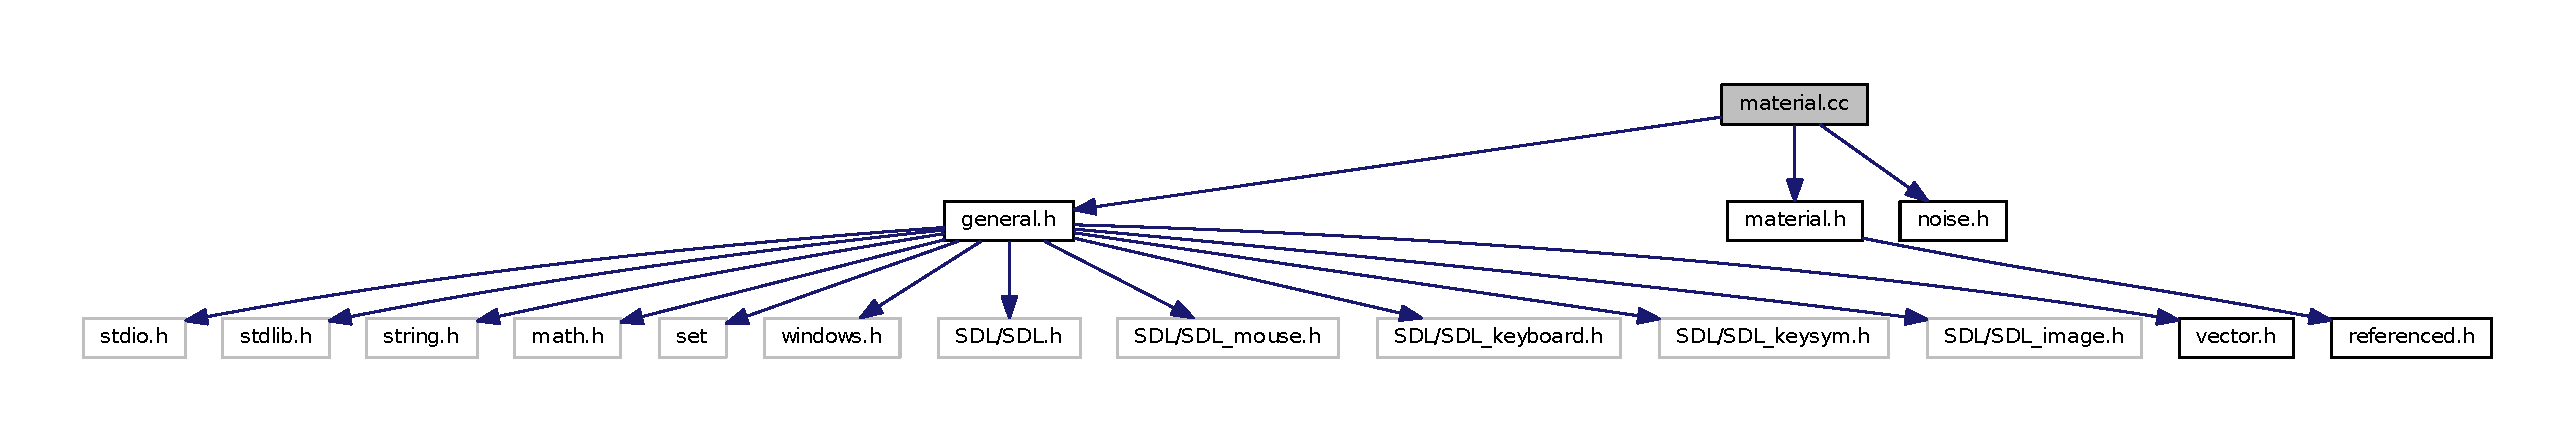
\includegraphics[width=350pt]{material_8cc__incl}
\end{center}
\end{figure}


\subsection{Detailed Description}
Implements all methods for all materials (\doxyref{Simple\+Material}{p.}{class_simple_material}, \doxyref{Checkerboard\+Material}{p.}{class_checkerboard_material}, \doxyref{Noise\+Material}{p.}{class_noise_material}, \doxyref{Material\+Map}{p.}{class_material_map}). 



Definition in file {\bf material.\+cc}.


\section{material.\+h File Reference}
\label{material_8h}\index{material.\+h@{material.\+h}}


Declares all methods for all materials (\doxyref{Simple\+Material}{p.}{class_simple_material}, \doxyref{Checkerboard\+Material}{p.}{class_checkerboard_material}, \doxyref{Noise\+Material}{p.}{class_noise_material}, \doxyref{Material\+Map}{p.}{class_material_map}).  


{\ttfamily \#include \char`\"{}referenced.\+h\char`\"{}}\\*
Include dependency graph for material.\+h\+:
\nopagebreak
\begin{figure}[H]
\begin{center}
\leavevmode
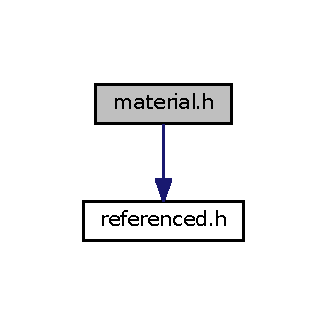
\includegraphics[width=157pt]{material_8h__incl}
\end{center}
\end{figure}
This graph shows which files directly or indirectly include this file\+:
\nopagebreak
\begin{figure}[H]
\begin{center}
\leavevmode
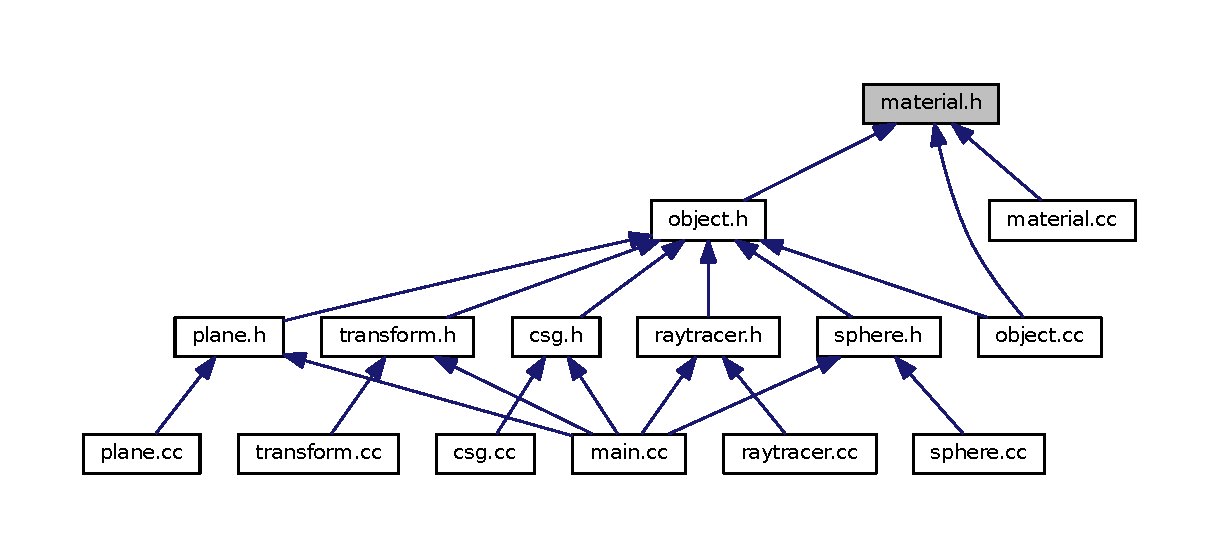
\includegraphics[width=350pt]{material_8h__dep__incl}
\end{center}
\end{figure}
\subsection*{Classes}
\begin{DoxyCompactItemize}
\item 
class {\bf Lighting\+Properties}
\begin{DoxyCompactList}\small\item\em Stores lighting properties used for Phong lighting, reflections and transparancy. \end{DoxyCompactList}\item 
class {\bf Material}
\begin{DoxyCompactList}\small\item\em Abstract base class for all materials. \end{DoxyCompactList}\item 
class {\bf Simple\+Material}
\begin{DoxyCompactList}\small\item\em Implements a simple material with the same properties over all of the whole object. \end{DoxyCompactList}\item 
class {\bf Checkerboard\+Material}
\begin{DoxyCompactList}\small\item\em A checkerboard pattern material. \end{DoxyCompactList}\item 
class {\bf Noise\+Material}
\begin{DoxyCompactList}\small\item\em Creates gray noise all over the object. \end{DoxyCompactList}\item 
class {\bf Material\+Map}
\begin{DoxyCompactList}\small\item\em Generic function mapped material. \end{DoxyCompactList}\end{DoxyCompactItemize}
\subsection*{Macros}
\begin{DoxyCompactItemize}
\item 
\#define {\bf M\+A\+X\+\_\+\+M\+A\+T\+E\+R\+I\+A\+L\+\_\+\+M\+A\+P\+\_\+\+N\+O\+D\+E\+S}~16
\end{DoxyCompactItemize}


\subsection{Detailed Description}
Declares all methods for all materials (\doxyref{Simple\+Material}{p.}{class_simple_material}, \doxyref{Checkerboard\+Material}{p.}{class_checkerboard_material}, \doxyref{Noise\+Material}{p.}{class_noise_material}, \doxyref{Material\+Map}{p.}{class_material_map}). 



Definition in file {\bf material.\+h}.



\subsection{Macro Definition Documentation}
\index{material.\+h@{material.\+h}!M\+A\+X\+\_\+\+M\+A\+T\+E\+R\+I\+A\+L\+\_\+\+M\+A\+P\+\_\+\+N\+O\+D\+E\+S@{M\+A\+X\+\_\+\+M\+A\+T\+E\+R\+I\+A\+L\+\_\+\+M\+A\+P\+\_\+\+N\+O\+D\+E\+S}}
\index{M\+A\+X\+\_\+\+M\+A\+T\+E\+R\+I\+A\+L\+\_\+\+M\+A\+P\+\_\+\+N\+O\+D\+E\+S@{M\+A\+X\+\_\+\+M\+A\+T\+E\+R\+I\+A\+L\+\_\+\+M\+A\+P\+\_\+\+N\+O\+D\+E\+S}!material.\+h@{material.\+h}}
\subsubsection[{M\+A\+X\+\_\+\+M\+A\+T\+E\+R\+I\+A\+L\+\_\+\+M\+A\+P\+\_\+\+N\+O\+D\+E\+S}]{\setlength{\rightskip}{0pt plus 5cm}\#define M\+A\+X\+\_\+\+M\+A\+T\+E\+R\+I\+A\+L\+\_\+\+M\+A\+P\+\_\+\+N\+O\+D\+E\+S~16}\label{material_8h_a6efc58c94fdf4d4fa45052aeaf308e9d}


Definition at line 93 of file material.\+h.


\section{noise.\+cc File Reference}
\label{noise_8cc}\index{noise.\+cc@{noise.\+cc}}


Implements functions for computing semi-\/random noise in 2-\/5 dimensions.  


{\ttfamily \#include \char`\"{}noise.\+h\char`\"{}}\\*
{\ttfamily \#include \char`\"{}stdlib.\+h\char`\"{}}\\*
Include dependency graph for noise.\+cc\+:
\nopagebreak
\begin{figure}[H]
\begin{center}
\leavevmode
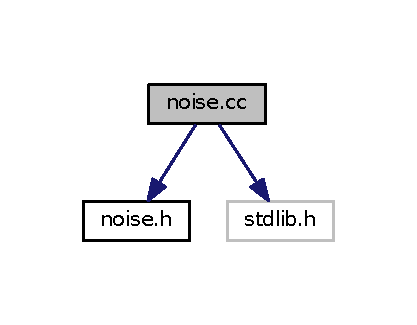
\includegraphics[width=200pt]{noise_8cc__incl}
\end{center}
\end{figure}
\subsection*{Functions}
\begin{DoxyCompactItemize}
\item 
void {\bf init\+Noise} ()
\item 
double {\bf semi\+Rand} (int x)
\item 
double {\bf semi\+Rand} (int x, int y)
\item 
double {\bf semi\+Rand} (int x, int y, int z)
\item 
double {\bf semi\+Rand} (int x, int y, int z, int w)
\item 
double {\bf semi\+Rand} (int x, int y, int z, int w, int h)
\item 
double {\bf noise} (double a)
\item 
double {\bf noise} (double a, double b)
\item 
double {\bf noise} (double a, double b, double c)
\item 
double {\bf noise} (double a, double b, double c, double d)
\end{DoxyCompactItemize}
\subsection*{Variables}
\begin{DoxyCompactItemize}
\item 
int {\bf rand\+Data} [5][1024]
\end{DoxyCompactItemize}


\subsection{Detailed Description}
Implements functions for computing semi-\/random noise in 2-\/5 dimensions. 



Definition in file {\bf noise.\+cc}.



\subsection{Function Documentation}
\index{noise.\+cc@{noise.\+cc}!init\+Noise@{init\+Noise}}
\index{init\+Noise@{init\+Noise}!noise.\+cc@{noise.\+cc}}
\subsubsection[{init\+Noise}]{\setlength{\rightskip}{0pt plus 5cm}void init\+Noise (
\begin{DoxyParamCaption}
{}
\end{DoxyParamCaption}
)}\label{noise_8cc_a9299630a0ca23186b81dab1828bf5927}


Definition at line 30 of file noise.\+cc.



References rand\+Data.



Referenced by main().

\index{noise.\+cc@{noise.\+cc}!noise@{noise}}
\index{noise@{noise}!noise.\+cc@{noise.\+cc}}
\subsubsection[{noise}]{\setlength{\rightskip}{0pt plus 5cm}double noise (
\begin{DoxyParamCaption}
\item[{double}]{a}
\end{DoxyParamCaption}
)}\label{noise_8cc_a428339e2af3692af4e843ffb1bf98191}


Definition at line 52 of file noise.\+cc.



References semi\+Rand().



Referenced by Noise\+Material\+::get\+Lighting\+Properties(), and Material\+Map\+::get\+Lighting\+Properties().

\index{noise.\+cc@{noise.\+cc}!noise@{noise}}
\index{noise@{noise}!noise.\+cc@{noise.\+cc}}
\subsubsection[{noise}]{\setlength{\rightskip}{0pt plus 5cm}double noise (
\begin{DoxyParamCaption}
\item[{double}]{a, }
\item[{double}]{b}
\end{DoxyParamCaption}
)}\label{noise_8cc_a88e8dfd1938c049c55aef61a169434cc}


Definition at line 59 of file noise.\+cc.



References semi\+Rand().

\index{noise.\+cc@{noise.\+cc}!noise@{noise}}
\index{noise@{noise}!noise.\+cc@{noise.\+cc}}
\subsubsection[{noise}]{\setlength{\rightskip}{0pt plus 5cm}double noise (
\begin{DoxyParamCaption}
\item[{double}]{a, }
\item[{double}]{b, }
\item[{double}]{c}
\end{DoxyParamCaption}
)}\label{noise_8cc_a9ce7e9860aa196876c2f2b14ff0fc3c5}


Definition at line 69 of file noise.\+cc.



References semi\+Rand().

\index{noise.\+cc@{noise.\+cc}!noise@{noise}}
\index{noise@{noise}!noise.\+cc@{noise.\+cc}}
\subsubsection[{noise}]{\setlength{\rightskip}{0pt plus 5cm}double noise (
\begin{DoxyParamCaption}
\item[{double}]{a, }
\item[{double}]{b, }
\item[{double}]{c, }
\item[{double}]{d}
\end{DoxyParamCaption}
)}\label{noise_8cc_a6f052c9b1f6a59feaad72965623998ce}


Definition at line 84 of file noise.\+cc.



References semi\+Rand().

\index{noise.\+cc@{noise.\+cc}!semi\+Rand@{semi\+Rand}}
\index{semi\+Rand@{semi\+Rand}!noise.\+cc@{noise.\+cc}}
\subsubsection[{semi\+Rand}]{\setlength{\rightskip}{0pt plus 5cm}double semi\+Rand (
\begin{DoxyParamCaption}
\item[{int}]{x}
\end{DoxyParamCaption}
)\hspace{0.3cm}{\ttfamily [inline]}}\label{noise_8cc_afacdaeba96485f0c16b866715f5784f8}


Definition at line 36 of file noise.\+cc.



References rand\+Data.



Referenced by noise().

\index{noise.\+cc@{noise.\+cc}!semi\+Rand@{semi\+Rand}}
\index{semi\+Rand@{semi\+Rand}!noise.\+cc@{noise.\+cc}}
\subsubsection[{semi\+Rand}]{\setlength{\rightskip}{0pt plus 5cm}double semi\+Rand (
\begin{DoxyParamCaption}
\item[{int}]{x, }
\item[{int}]{y}
\end{DoxyParamCaption}
)\hspace{0.3cm}{\ttfamily [inline]}}\label{noise_8cc_a93ff7fcabba013d8bb39343415c04e84}


Definition at line 39 of file noise.\+cc.



References rand\+Data.

\index{noise.\+cc@{noise.\+cc}!semi\+Rand@{semi\+Rand}}
\index{semi\+Rand@{semi\+Rand}!noise.\+cc@{noise.\+cc}}
\subsubsection[{semi\+Rand}]{\setlength{\rightskip}{0pt plus 5cm}double semi\+Rand (
\begin{DoxyParamCaption}
\item[{int}]{x, }
\item[{int}]{y, }
\item[{int}]{z}
\end{DoxyParamCaption}
)\hspace{0.3cm}{\ttfamily [inline]}}\label{noise_8cc_aae38f8baa10d1fd4d5c5fdfc126934d7}


Definition at line 42 of file noise.\+cc.



References rand\+Data.

\index{noise.\+cc@{noise.\+cc}!semi\+Rand@{semi\+Rand}}
\index{semi\+Rand@{semi\+Rand}!noise.\+cc@{noise.\+cc}}
\subsubsection[{semi\+Rand}]{\setlength{\rightskip}{0pt plus 5cm}double semi\+Rand (
\begin{DoxyParamCaption}
\item[{int}]{x, }
\item[{int}]{y, }
\item[{int}]{z, }
\item[{int}]{w}
\end{DoxyParamCaption}
)\hspace{0.3cm}{\ttfamily [inline]}}\label{noise_8cc_a9a8ec4a421113dc3cb57a5a908cd27b3}


Definition at line 45 of file noise.\+cc.



References rand\+Data.

\index{noise.\+cc@{noise.\+cc}!semi\+Rand@{semi\+Rand}}
\index{semi\+Rand@{semi\+Rand}!noise.\+cc@{noise.\+cc}}
\subsubsection[{semi\+Rand}]{\setlength{\rightskip}{0pt plus 5cm}double semi\+Rand (
\begin{DoxyParamCaption}
\item[{int}]{x, }
\item[{int}]{y, }
\item[{int}]{z, }
\item[{int}]{w, }
\item[{int}]{h}
\end{DoxyParamCaption}
)\hspace{0.3cm}{\ttfamily [inline]}}\label{noise_8cc_a72d8656f6222adb94bfc3b3dea79364a}


Definition at line 48 of file noise.\+cc.



References rand\+Data.



\subsection{Variable Documentation}
\index{noise.\+cc@{noise.\+cc}!rand\+Data@{rand\+Data}}
\index{rand\+Data@{rand\+Data}!noise.\+cc@{noise.\+cc}}
\subsubsection[{rand\+Data}]{\setlength{\rightskip}{0pt plus 5cm}int rand\+Data[5][1024]}\label{noise_8cc_a52301da5478980975ca1196d6e0e55e1}


Definition at line 28 of file noise.\+cc.



Referenced by init\+Noise(), and semi\+Rand().


\section{noise.\+h File Reference}
\label{noise_8h}\index{noise.\+h@{noise.\+h}}


Declares functions for computing semi-\/random noise in 2-\/5 dimensions.  


This graph shows which files directly or indirectly include this file\+:
\nopagebreak
\begin{figure}[H]
\begin{center}
\leavevmode
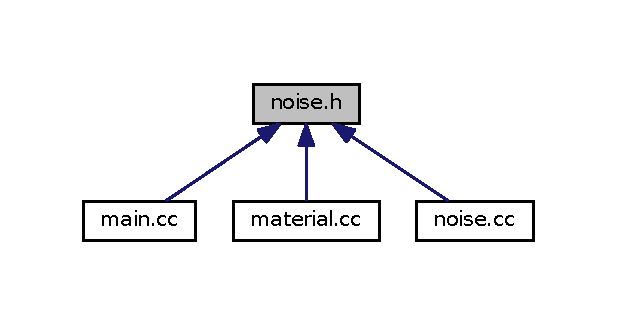
\includegraphics[width=296pt]{noise_8h__dep__incl}
\end{center}
\end{figure}
\subsection*{Functions}
\begin{DoxyCompactItemize}
\item 
void {\bf init\+Noise} ()
\item 
double {\bf noise} (double a)
\item 
double {\bf noise} (double a, double b)
\item 
double {\bf noise} (double a, double b, double c)
\item 
double {\bf noise} (double a, double b, double c, double d)
\end{DoxyCompactItemize}


\subsection{Detailed Description}
Declares functions for computing semi-\/random noise in 2-\/5 dimensions. 



Definition in file {\bf noise.\+h}.



\subsection{Function Documentation}
\index{noise.\+h@{noise.\+h}!init\+Noise@{init\+Noise}}
\index{init\+Noise@{init\+Noise}!noise.\+h@{noise.\+h}}
\subsubsection[{init\+Noise}]{\setlength{\rightskip}{0pt plus 5cm}void init\+Noise (
\begin{DoxyParamCaption}
{}
\end{DoxyParamCaption}
)}\label{noise_8h_a9299630a0ca23186b81dab1828bf5927}


Definition at line 30 of file noise.\+cc.



References rand\+Data.



Referenced by main().

\index{noise.\+h@{noise.\+h}!noise@{noise}}
\index{noise@{noise}!noise.\+h@{noise.\+h}}
\subsubsection[{noise}]{\setlength{\rightskip}{0pt plus 5cm}double noise (
\begin{DoxyParamCaption}
\item[{double}]{a}
\end{DoxyParamCaption}
)}\label{noise_8h_a428339e2af3692af4e843ffb1bf98191}


Definition at line 52 of file noise.\+cc.



References semi\+Rand().



Referenced by Noise\+Material\+::get\+Lighting\+Properties(), and Material\+Map\+::get\+Lighting\+Properties().

\index{noise.\+h@{noise.\+h}!noise@{noise}}
\index{noise@{noise}!noise.\+h@{noise.\+h}}
\subsubsection[{noise}]{\setlength{\rightskip}{0pt plus 5cm}double noise (
\begin{DoxyParamCaption}
\item[{double}]{a, }
\item[{double}]{b}
\end{DoxyParamCaption}
)}\label{noise_8h_a88e8dfd1938c049c55aef61a169434cc}


Definition at line 59 of file noise.\+cc.



References semi\+Rand().

\index{noise.\+h@{noise.\+h}!noise@{noise}}
\index{noise@{noise}!noise.\+h@{noise.\+h}}
\subsubsection[{noise}]{\setlength{\rightskip}{0pt plus 5cm}double noise (
\begin{DoxyParamCaption}
\item[{double}]{a, }
\item[{double}]{b, }
\item[{double}]{c}
\end{DoxyParamCaption}
)}\label{noise_8h_a9ce7e9860aa196876c2f2b14ff0fc3c5}


Definition at line 69 of file noise.\+cc.



References semi\+Rand().

\index{noise.\+h@{noise.\+h}!noise@{noise}}
\index{noise@{noise}!noise.\+h@{noise.\+h}}
\subsubsection[{noise}]{\setlength{\rightskip}{0pt plus 5cm}double noise (
\begin{DoxyParamCaption}
\item[{double}]{a, }
\item[{double}]{b, }
\item[{double}]{c, }
\item[{double}]{d}
\end{DoxyParamCaption}
)}\label{noise_8h_a6f052c9b1f6a59feaad72965623998ce}


Definition at line 84 of file noise.\+cc.



References semi\+Rand().


\section{object.\+cc File Reference}
\label{object_8cc}\index{object.\+cc@{object.\+cc}}


Implements all generic methods for all raytracable objects.  


{\ttfamily \#include \char`\"{}general.\+h\char`\"{}}\\*
{\ttfamily \#include \char`\"{}material.\+h\char`\"{}}\\*
{\ttfamily \#include \char`\"{}object.\+h\char`\"{}}\\*
Include dependency graph for object.\+cc\+:
\nopagebreak
\begin{figure}[H]
\begin{center}
\leavevmode
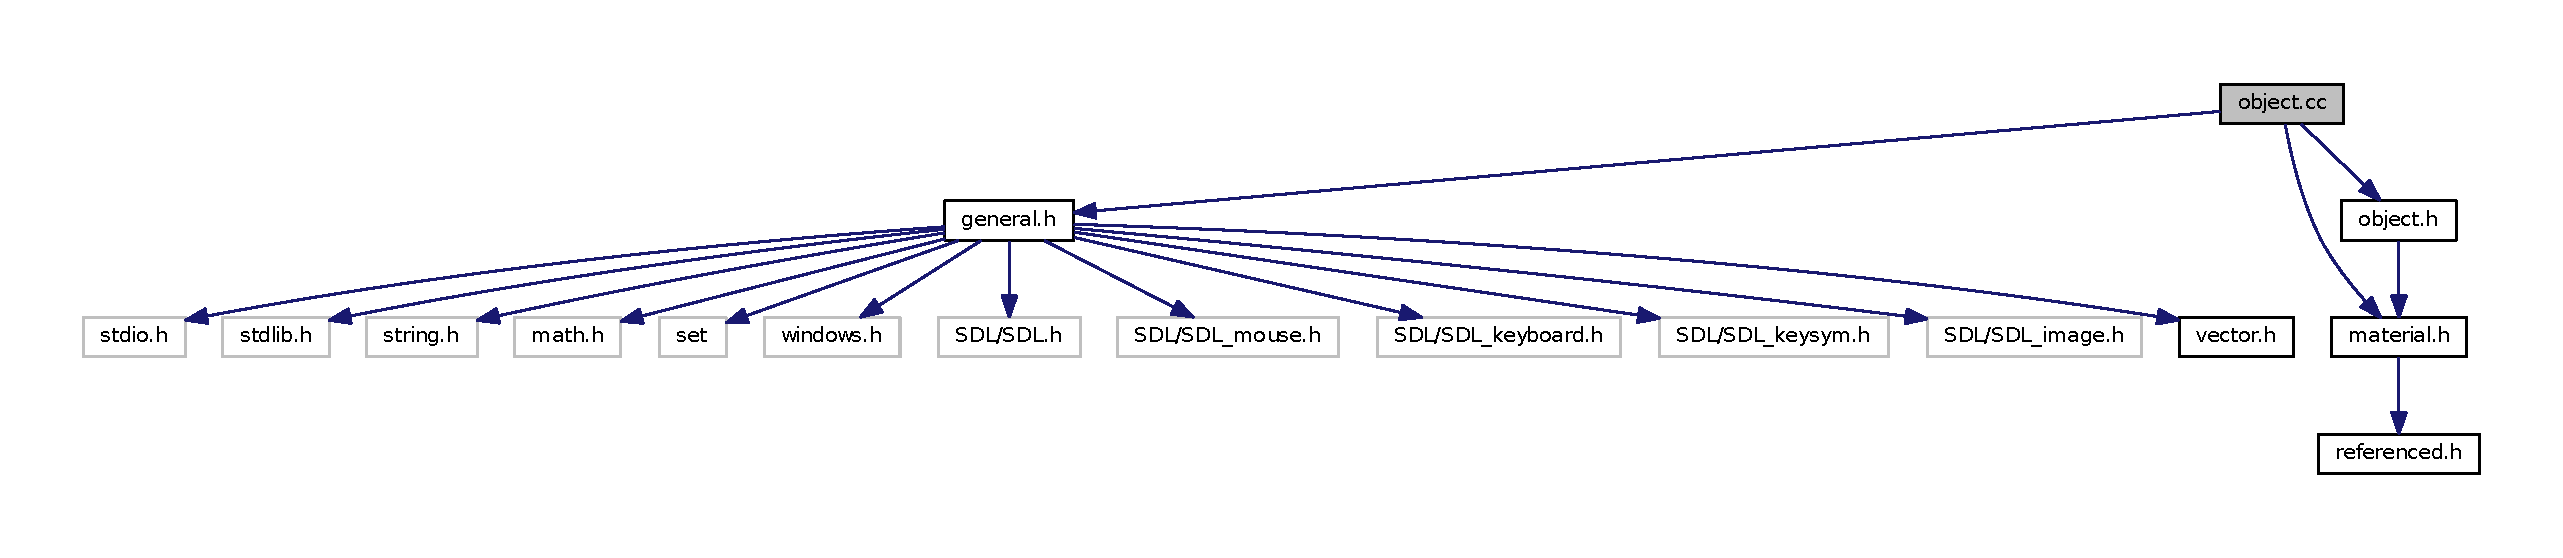
\includegraphics[width=350pt]{object_8cc__incl}
\end{center}
\end{figure}


\subsection{Detailed Description}
Implements all generic methods for all raytracable objects. 



Definition in file {\bf object.\+cc}.


\section{object.\+h File Reference}
\label{object_8h}\index{object.\+h@{object.\+h}}


Declares all generic methods for all raytracable objects.  


{\ttfamily \#include \char`\"{}material.\+h\char`\"{}}\\*
Include dependency graph for object.\+h\+:
\nopagebreak
\begin{figure}[H]
\begin{center}
\leavevmode
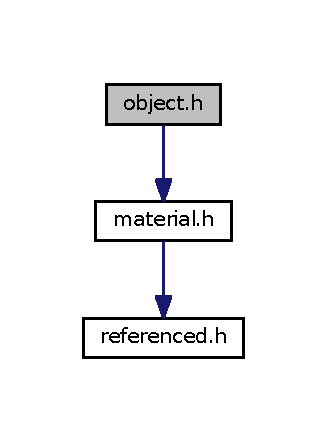
\includegraphics[width=157pt]{object_8h__incl}
\end{center}
\end{figure}
This graph shows which files directly or indirectly include this file\+:
\nopagebreak
\begin{figure}[H]
\begin{center}
\leavevmode
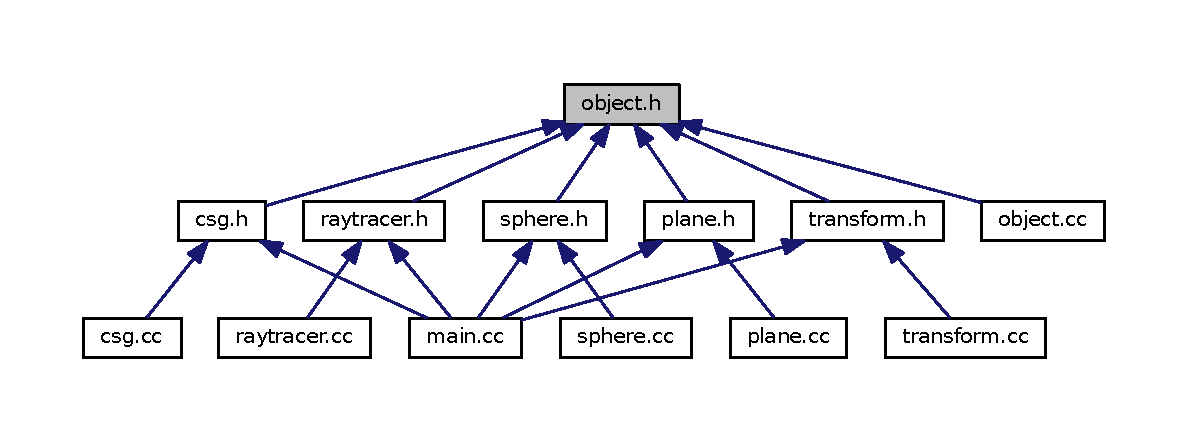
\includegraphics[width=350pt]{object_8h__dep__incl}
\end{center}
\end{figure}
\subsection*{Classes}
\begin{DoxyCompactItemize}
\item 
class {\bf Object}
\begin{DoxyCompactList}\small\item\em Abstract base class for all renderable objects. \end{DoxyCompactList}\end{DoxyCompactItemize}
\subsection*{Macros}
\begin{DoxyCompactItemize}
\item 
\#define {\bf M\+A\+X\+\_\+\+D\+I\+S\+T\+A\+N\+C\+E}~1e9
\end{DoxyCompactItemize}


\subsection{Detailed Description}
Declares all generic methods for all raytracable objects. 



Definition in file {\bf object.\+h}.



\subsection{Macro Definition Documentation}
\index{object.\+h@{object.\+h}!M\+A\+X\+\_\+\+D\+I\+S\+T\+A\+N\+C\+E@{M\+A\+X\+\_\+\+D\+I\+S\+T\+A\+N\+C\+E}}
\index{M\+A\+X\+\_\+\+D\+I\+S\+T\+A\+N\+C\+E@{M\+A\+X\+\_\+\+D\+I\+S\+T\+A\+N\+C\+E}!object.\+h@{object.\+h}}
\subsubsection[{M\+A\+X\+\_\+\+D\+I\+S\+T\+A\+N\+C\+E}]{\setlength{\rightskip}{0pt plus 5cm}\#define M\+A\+X\+\_\+\+D\+I\+S\+T\+A\+N\+C\+E~1e9}\label{object_8h_a08e4da5f3d0c7936fa52467f40e4b6aa}


Definition at line 32 of file object.\+h.



Referenced by Plane\+::line\+Test(), Sphere\+::line\+Test(), Intersection\+::line\+Test(), and Raytracer\+::raytrace().


\section{plane.\+cc File Reference}
\label{plane_8cc}\index{plane.\+cc@{plane.\+cc}}


Implements all methods for the \doxyref{Plane}{p.}{class_plane} class.  


{\ttfamily \#include \char`\"{}general.\+h\char`\"{}}\\*
{\ttfamily \#include \char`\"{}plane.\+h\char`\"{}}\\*
Include dependency graph for plane.\+cc\+:
\nopagebreak
\begin{figure}[H]
\begin{center}
\leavevmode
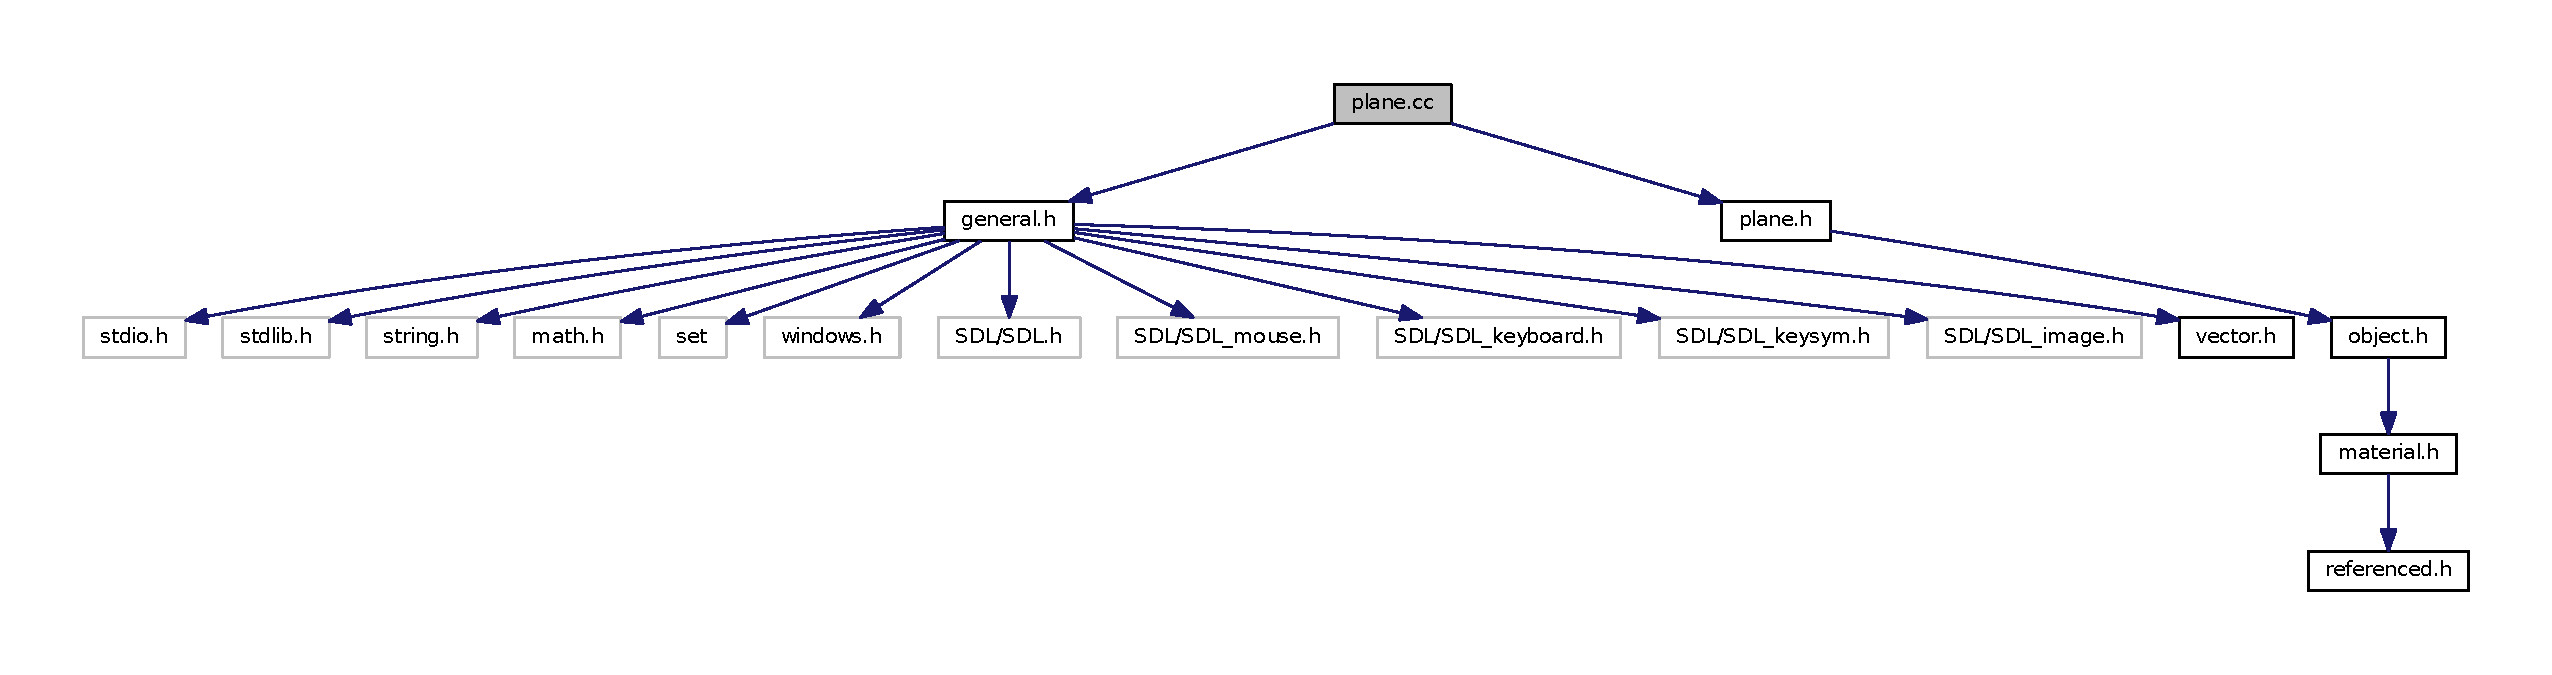
\includegraphics[width=350pt]{plane_8cc__incl}
\end{center}
\end{figure}


\subsection{Detailed Description}
Implements all methods for the \doxyref{Plane}{p.}{class_plane} class. 



Definition in file {\bf plane.\+cc}.


\section{plane.\+h File Reference}
\label{plane_8h}\index{plane.\+h@{plane.\+h}}


Declares all methods for the \doxyref{Plane}{p.}{class_plane} class.  


{\ttfamily \#include \char`\"{}object.\+h\char`\"{}}\\*
Include dependency graph for plane.\+h\+:
\nopagebreak
\begin{figure}[H]
\begin{center}
\leavevmode
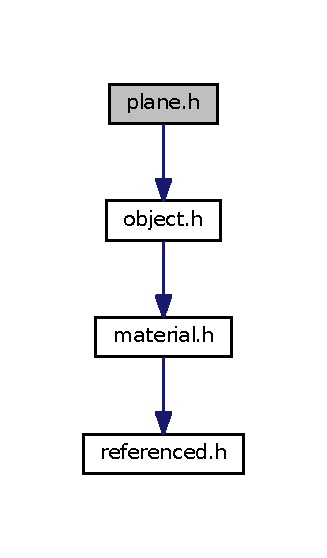
\includegraphics[width=157pt]{plane_8h__incl}
\end{center}
\end{figure}
This graph shows which files directly or indirectly include this file\+:
\nopagebreak
\begin{figure}[H]
\begin{center}
\leavevmode
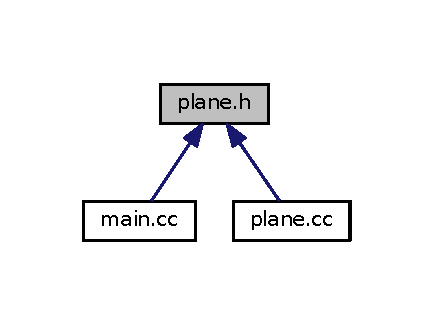
\includegraphics[width=208pt]{plane_8h__dep__incl}
\end{center}
\end{figure}
\subsection*{Classes}
\begin{DoxyCompactItemize}
\item 
class {\bf Plane}
\begin{DoxyCompactList}\small\item\em An infinite plane with given normal and offset from origo. \end{DoxyCompactList}\end{DoxyCompactItemize}


\subsection{Detailed Description}
Declares all methods for the \doxyref{Plane}{p.}{class_plane} class. 



Definition in file {\bf plane.\+h}.


\section{raytracer.\+cc File Reference}
\label{raytracer_8cc}\index{raytracer.\+cc@{raytracer.\+cc}}


Implements the main raytracing functionality for the \doxyref{Raytracer}{p.}{class_raytracer} class.  


{\ttfamily \#include \char`\"{}general.\+h\char`\"{}}\\*
{\ttfamily \#include \char`\"{}raytracer.\+h\char`\"{}}\\*
Include dependency graph for raytracer.\+cc\+:
\nopagebreak
\begin{figure}[H]
\begin{center}
\leavevmode
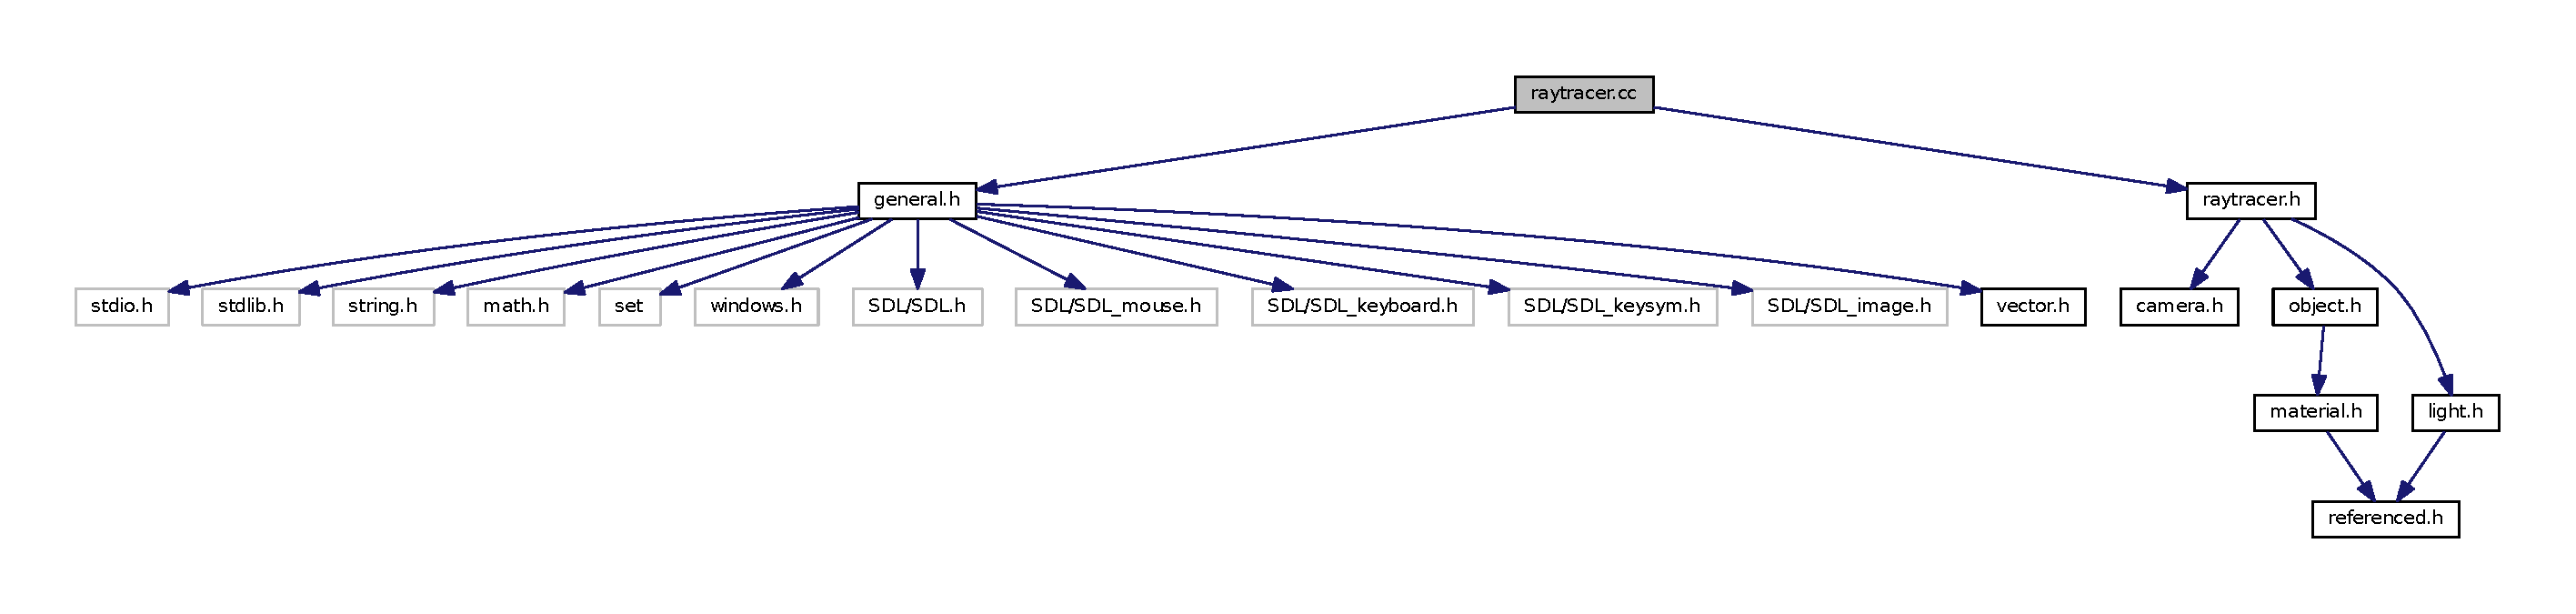
\includegraphics[width=350pt]{raytracer_8cc__incl}
\end{center}
\end{figure}
\subsection*{Variables}
\begin{DoxyCompactItemize}
\item 
int {\bf screen\+Width}
\item 
int {\bf screen\+Height}
\end{DoxyCompactItemize}


\subsection{Detailed Description}
Implements the main raytracing functionality for the \doxyref{Raytracer}{p.}{class_raytracer} class. 



Definition in file {\bf raytracer.\+cc}.



\subsection{Variable Documentation}
\index{raytracer.\+cc@{raytracer.\+cc}!screen\+Height@{screen\+Height}}
\index{screen\+Height@{screen\+Height}!raytracer.\+cc@{raytracer.\+cc}}
\subsubsection[{screen\+Height}]{\setlength{\rightskip}{0pt plus 5cm}int screen\+Height}\label{raytracer_8cc_a9ebc1dbd77788c4bfa27758a6725413f}


Definition at line 70 of file main.\+cc.



Referenced by do\+Redraw(), main(), and Raytracer\+::raytrace().

\index{raytracer.\+cc@{raytracer.\+cc}!screen\+Width@{screen\+Width}}
\index{screen\+Width@{screen\+Width}!raytracer.\+cc@{raytracer.\+cc}}
\subsubsection[{screen\+Width}]{\setlength{\rightskip}{0pt plus 5cm}int screen\+Width}\label{raytracer_8cc_ae50cb92a78d9e0a4f4bd718fc02bd294}


Definition at line 70 of file main.\+cc.



Referenced by do\+Redraw(), main(), and Raytracer\+::raytrace().


\section{raytracer.\+h File Reference}
\label{raytracer_8h}\index{raytracer.\+h@{raytracer.\+h}}


Declares the main raytracing functionality for the \doxyref{Raytracer}{p.}{class_raytracer} class.  


{\ttfamily \#include \char`\"{}camera.\+h\char`\"{}}\\*
{\ttfamily \#include \char`\"{}object.\+h\char`\"{}}\\*
{\ttfamily \#include \char`\"{}light.\+h\char`\"{}}\\*
Include dependency graph for raytracer.\+h\+:
\nopagebreak
\begin{figure}[H]
\begin{center}
\leavevmode
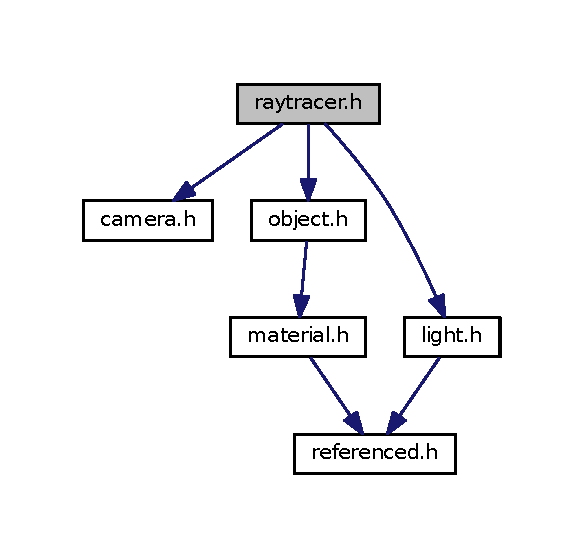
\includegraphics[width=280pt]{raytracer_8h__incl}
\end{center}
\end{figure}
This graph shows which files directly or indirectly include this file\+:
\nopagebreak
\begin{figure}[H]
\begin{center}
\leavevmode
\includegraphics[width=226pt]{raytracer_8h__dep__incl}
\end{center}
\end{figure}
\subsection*{Classes}
\begin{DoxyCompactItemize}
\item 
class {\bf Raytracer}
\begin{DoxyCompactList}\small\item\em Main class for performing all raytracing operations. \end{DoxyCompactList}\end{DoxyCompactItemize}


\subsection{Detailed Description}
Declares the main raytracing functionality for the \doxyref{Raytracer}{p.}{class_raytracer} class. 



Definition in file {\bf raytracer.\+h}.


\section{referenced.\+cc File Reference}
\label{referenced_8cc}\index{referenced.\+cc@{referenced.\+cc}}


Implements reference counters for all objects used by the raytracer via the \doxyref{Referenced\+Object}{p.}{class_referenced_object} class.  


{\ttfamily \#include \char`\"{}general.\+h\char`\"{}}\\*
{\ttfamily \#include \char`\"{}referenced.\+h\char`\"{}}\\*
Include dependency graph for referenced.\+cc\+:
\nopagebreak
\begin{figure}[H]
\begin{center}
\leavevmode
\includegraphics[width=350pt]{referenced_8cc__incl}
\end{center}
\end{figure}


\subsection{Detailed Description}
Implements reference counters for all objects used by the raytracer via the \doxyref{Referenced\+Object}{p.}{class_referenced_object} class. 



Definition in file {\bf referenced.\+cc}.


\section{referenced.\+h File Reference}
\label{referenced_8h}\index{referenced.\+h@{referenced.\+h}}


Implements reference counters for all objects used by the raytracer via the \doxyref{Referenced\+Object}{p.}{class_referenced_object} class.  


This graph shows which files directly or indirectly include this file\+:
\nopagebreak
\begin{figure}[H]
\begin{center}
\leavevmode
\includegraphics[width=350pt]{referenced_8h__dep__incl}
\end{center}
\end{figure}
\subsection*{Classes}
\begin{DoxyCompactItemize}
\item 
class {\bf Referenced\+Object}
\begin{DoxyCompactList}\small\item\em Base class for all objects which use a reference counter for memory management. \end{DoxyCompactList}\end{DoxyCompactItemize}


\subsection{Detailed Description}
Implements reference counters for all objects used by the raytracer via the \doxyref{Referenced\+Object}{p.}{class_referenced_object} class. 



Definition in file {\bf referenced.\+h}.


\section{sphere.\+cc File Reference}
\label{sphere_8cc}\index{sphere.\+cc@{sphere.\+cc}}


Implements all methods for the \doxyref{Sphere}{p.}{class_sphere} class.  


{\ttfamily \#include \char`\"{}general.\+h\char`\"{}}\\*
{\ttfamily \#include \char`\"{}sphere.\+h\char`\"{}}\\*
Include dependency graph for sphere.\+cc\+:
\nopagebreak
\begin{figure}[H]
\begin{center}
\leavevmode
\includegraphics[width=350pt]{sphere_8cc__incl}
\end{center}
\end{figure}


\subsection{Detailed Description}
Implements all methods for the \doxyref{Sphere}{p.}{class_sphere} class. 



Definition in file {\bf sphere.\+cc}.


\section{sphere.\+h File Reference}
\label{sphere_8h}\index{sphere.\+h@{sphere.\+h}}


Declares all methods for the \doxyref{Sphere}{p.}{class_sphere} class.  


{\ttfamily \#include \char`\"{}object.\+h\char`\"{}}\\*
Include dependency graph for sphere.\+h\+:
\nopagebreak
\begin{figure}[H]
\begin{center}
\leavevmode
\includegraphics[width=157pt]{sphere_8h__incl}
\end{center}
\end{figure}
This graph shows which files directly or indirectly include this file\+:
\nopagebreak
\begin{figure}[H]
\begin{center}
\leavevmode
\includegraphics[width=216pt]{sphere_8h__dep__incl}
\end{center}
\end{figure}
\subsection*{Classes}
\begin{DoxyCompactItemize}
\item 
class {\bf Sphere}
\begin{DoxyCompactList}\small\item\em A sphere of given radius. \end{DoxyCompactList}\end{DoxyCompactItemize}


\subsection{Detailed Description}
Declares all methods for the \doxyref{Sphere}{p.}{class_sphere} class. 



Definition in file {\bf sphere.\+h}.


\section{transform.\+cc File Reference}
\label{transform_8cc}\index{transform.\+cc@{transform.\+cc}}


Implements all methods for the \doxyref{Transform}{p.}{class_transform} class.  


{\ttfamily \#include \char`\"{}general.\+h\char`\"{}}\\*
{\ttfamily \#include \char`\"{}transform.\+h\char`\"{}}\\*
Include dependency graph for transform.\+cc\+:
\nopagebreak
\begin{figure}[H]
\begin{center}
\leavevmode
\includegraphics[width=350pt]{transform_8cc__incl}
\end{center}
\end{figure}


\subsection{Detailed Description}
Implements all methods for the \doxyref{Transform}{p.}{class_transform} class. 



Definition in file {\bf transform.\+cc}.


\section{transform.\+h File Reference}
\label{transform_8h}\index{transform.\+h@{transform.\+h}}


Declares all methods for the \doxyref{Transform}{p.}{class_transform} class.  


{\ttfamily \#include \char`\"{}object.\+h\char`\"{}}\\*
Include dependency graph for transform.\+h\+:
\nopagebreak
\begin{figure}[H]
\begin{center}
\leavevmode
\includegraphics[width=157pt]{transform_8h__incl}
\end{center}
\end{figure}
This graph shows which files directly or indirectly include this file\+:
\nopagebreak
\begin{figure}[H]
\begin{center}
\leavevmode
\includegraphics[width=230pt]{transform_8h__dep__incl}
\end{center}
\end{figure}
\subsection*{Classes}
\begin{DoxyCompactItemize}
\item 
class {\bf Transform}
\begin{DoxyCompactList}\small\item\em Represents generic affine transformations. \end{DoxyCompactList}\end{DoxyCompactItemize}


\subsection{Detailed Description}
Declares all methods for the \doxyref{Transform}{p.}{class_transform} class. 



Definition in file {\bf transform.\+h}.


\section{vector.\+cc File Reference}
\label{vector_8cc}\index{vector.\+cc@{vector.\+cc}}


Implements some miscellaneous.  


{\ttfamily \#include $<$stdio.\+h$>$}\\*
{\ttfamily \#include $<$math.\+h$>$}\\*
{\ttfamily \#include \char`\"{}general.\+h\char`\"{}}\\*
{\ttfamily \#include \char`\"{}vector.\+h\char`\"{}}\\*
Include dependency graph for vector.\+cc\+:
\nopagebreak
\begin{figure}[H]
\begin{center}
\leavevmode
\includegraphics[width=350pt]{vector_8cc__incl}
\end{center}
\end{figure}
\subsection*{Functions}
\begin{DoxyCompactItemize}
\item 
void {\bf add} (const double A[3], const double B[3], double C[3])
\item 
void {\bf sub} (const double A[3], const double B[3], double C[3])
\item 
void {\bf normalize} (double C[3])
\item 
double {\bf length} (double A[3])
\item 
void {\bf cross\+Product} (const double A[3], const double B[3], double C[3])
\item 
double {\bf dot\+Product} (const double A[3], const double B[3])
\item 
void {\bf debug\+Matrix} ({\bf Matrix4d} m)
\begin{DoxyCompactList}\small\item\em Print out a matrix in a human readable form. \end{DoxyCompactList}\item 
void {\bf matrix\+Mult} ({\bf Matrix4d} A, {\bf Matrix4d} B, {\bf Matrix4d} C)
\item 
void {\bf homogenise} (double A[4], double C[3])
\begin{DoxyCompactList}\small\item\em Homogeneis A and assign to C. \end{DoxyCompactList}\item 
void {\bf use\+Matrix} ({\bf Matrix4d} A, const double B[4], double C[4])
\begin{DoxyCompactList}\small\item\em Assign to C the value M $\ast$ A. \end{DoxyCompactList}\item 
void {\bf use\+Matrix} ({\bf Matrix3d} A, const double B[3], double C[3])
\begin{DoxyCompactList}\small\item\em Assign to C the value M $\ast$ A. \end{DoxyCompactList}\item 
void {\bf use\+Matrix} ({\bf Matrix4d} m, const double x, const double y, const double z, double C[3])
\begin{DoxyCompactList}\small\item\em Assign to C the value M $\ast$ $<$x,y,z$>$ \end{DoxyCompactList}\item 
void {\bf use\+Matrix} ({\bf Matrix4d} m, const double x, const double y, const double z, float C[3])
\begin{DoxyCompactList}\small\item\em Assign to C the value M $\ast$ $<$x,y,z$>$ \end{DoxyCompactList}\item 
void {\bf assign} (const {\bf Matrix4d} A, {\bf Matrix4d} C)
\item 
void {\bf assign} (const double A[3], double C[3])
\item 
void {\bf assign} (const float A[3], float C[3])
\item 
void {\bf identity\+Matrix} ({\bf Matrix4d} m)
\item 
void {\bf rotate\+Matrix\+X} (double v, {\bf Matrix4d} m)
\item 
void {\bf rotate\+Matrix\+Y} (double v, {\bf Matrix4d} m)
\item 
void {\bf rotate\+Matrix\+Z} (double v, {\bf Matrix4d} m)
\item 
void {\bf translate\+X\+Y\+Z} (double x, double y, double z, {\bf Matrix4d} m)
\item 
void {\bf zero} (double v[3])
\end{DoxyCompactItemize}


\subsection{Detailed Description}
Implements some miscellaneous. 

math vector/matrix operations. 

Definition in file {\bf vector.\+cc}.



\subsection{Function Documentation}
\index{vector.\+cc@{vector.\+cc}!add@{add}}
\index{add@{add}!vector.\+cc@{vector.\+cc}}
\subsubsection[{add}]{\setlength{\rightskip}{0pt plus 5cm}void add (
\begin{DoxyParamCaption}
\item[{const double}]{A[3], }
\item[{const double}]{B[3], }
\item[{double}]{C[3]}
\end{DoxyParamCaption}
)}\label{vector_8cc_ab857ae51cb219acd3215c72b632e1ca1}


Definition at line 33 of file vector.\+cc.

\index{vector.\+cc@{vector.\+cc}!assign@{assign}}
\index{assign@{assign}!vector.\+cc@{vector.\+cc}}
\subsubsection[{assign}]{\setlength{\rightskip}{0pt plus 5cm}void assign (
\begin{DoxyParamCaption}
\item[{const {\bf Matrix4d}}]{A, }
\item[{{\bf Matrix4d}}]{C}
\end{DoxyParamCaption}
)}\label{vector_8cc_ae3e07fa99d972082756ecc59df6aa880}


Definition at line 138 of file vector.\+cc.



Referenced by Plane\+::get\+Normal(), Sphere\+::get\+Normal(), Transform\+::get\+Normal(), Camera\+::get\+Pixel\+Ray(), Light\+::\+Light(), Intersection\+::line\+Test(), Plane\+::\+Plane(), rotate\+Matrix\+X(), rotate\+Matrix\+Y(), rotate\+Matrix\+Z(), Transform\+::scale(), Raytracer\+::set\+Ambient\+Light(), Raytracer\+::set\+Background(), Camera\+::set\+Forward(), Camera\+::set\+Origin(), Camera\+::set\+Right(), Camera\+::set\+Up(), Transform\+::translate(), and translate\+X\+Y\+Z().

\index{vector.\+cc@{vector.\+cc}!assign@{assign}}
\index{assign@{assign}!vector.\+cc@{vector.\+cc}}
\subsubsection[{assign}]{\setlength{\rightskip}{0pt plus 5cm}void assign (
\begin{DoxyParamCaption}
\item[{const double}]{A[3], }
\item[{double}]{C[3]}
\end{DoxyParamCaption}
)}\label{vector_8cc_a415ccce4f7df55b93408b27871807ba5}


Definition at line 146 of file vector.\+cc.

\index{vector.\+cc@{vector.\+cc}!assign@{assign}}
\index{assign@{assign}!vector.\+cc@{vector.\+cc}}
\subsubsection[{assign}]{\setlength{\rightskip}{0pt plus 5cm}void assign (
\begin{DoxyParamCaption}
\item[{const float}]{A[3], }
\item[{float}]{C[3]}
\end{DoxyParamCaption}
)}\label{vector_8cc_a53c132865e39e6c608d18c0adaad7f9d}


Definition at line 149 of file vector.\+cc.

\index{vector.\+cc@{vector.\+cc}!cross\+Product@{cross\+Product}}
\index{cross\+Product@{cross\+Product}!vector.\+cc@{vector.\+cc}}
\subsubsection[{cross\+Product}]{\setlength{\rightskip}{0pt plus 5cm}void cross\+Product (
\begin{DoxyParamCaption}
\item[{const double}]{A[3], }
\item[{const double}]{B[3], }
\item[{double}]{C[3]}
\end{DoxyParamCaption}
)}\label{vector_8cc_a28db7f272927a82733e31e964c0137fc}


Definition at line 51 of file vector.\+cc.



Referenced by Camera\+::set\+Focus().

\index{vector.\+cc@{vector.\+cc}!debug\+Matrix@{debug\+Matrix}}
\index{debug\+Matrix@{debug\+Matrix}!vector.\+cc@{vector.\+cc}}
\subsubsection[{debug\+Matrix}]{\setlength{\rightskip}{0pt plus 5cm}void debug\+Matrix (
\begin{DoxyParamCaption}
\item[{{\bf Matrix4d}}]{m}
\end{DoxyParamCaption}
)}\label{vector_8cc_a0a934c767332cb32532a8f56a89e37fd}


Print out a matrix in a human readable form. 



Definition at line 66 of file vector.\+cc.

\index{vector.\+cc@{vector.\+cc}!dot\+Product@{dot\+Product}}
\index{dot\+Product@{dot\+Product}!vector.\+cc@{vector.\+cc}}
\subsubsection[{dot\+Product}]{\setlength{\rightskip}{0pt plus 5cm}double dot\+Product (
\begin{DoxyParamCaption}
\item[{const double}]{A[3], }
\item[{const double}]{B[3]}
\end{DoxyParamCaption}
)}\label{vector_8cc_ae7b1006834d412eb2a8ca1af92e767a5}


Definition at line 58 of file vector.\+cc.



Referenced by Plane\+::is\+Inside(), Sphere\+::is\+Inside(), Plane\+::line\+Test(), Sphere\+::line\+Test(), Raytracer\+::raytrace(), and Camera\+::set\+Focus().

\index{vector.\+cc@{vector.\+cc}!homogenise@{homogenise}}
\index{homogenise@{homogenise}!vector.\+cc@{vector.\+cc}}
\subsubsection[{homogenise}]{\setlength{\rightskip}{0pt plus 5cm}void homogenise (
\begin{DoxyParamCaption}
\item[{double}]{A[4], }
\item[{double}]{C[3]}
\end{DoxyParamCaption}
)}\label{vector_8cc_a30c57bce7cfe7b00bb69e776a4d1823c}


Homogeneis A and assign to C. 



Definition at line 84 of file vector.\+cc.

\index{vector.\+cc@{vector.\+cc}!identity\+Matrix@{identity\+Matrix}}
\index{identity\+Matrix@{identity\+Matrix}!vector.\+cc@{vector.\+cc}}
\subsubsection[{identity\+Matrix}]{\setlength{\rightskip}{0pt plus 5cm}void identity\+Matrix (
\begin{DoxyParamCaption}
\item[{{\bf Matrix4d}}]{m}
\end{DoxyParamCaption}
)}\label{vector_8cc_aea238a0421832979d7b70e30ce0145b2}


Definition at line 151 of file vector.\+cc.



Referenced by Transform\+::identity(), Transform\+::scale(), Transform\+::\+Transform(), and Transform\+::translate().

\index{vector.\+cc@{vector.\+cc}!length@{length}}
\index{length@{length}!vector.\+cc@{vector.\+cc}}
\subsubsection[{length}]{\setlength{\rightskip}{0pt plus 5cm}double length (
\begin{DoxyParamCaption}
\item[{double}]{A[3]}
\end{DoxyParamCaption}
)}\label{vector_8cc_a4297922edc1bf5ddd0d690d8320c5342}


Definition at line 47 of file vector.\+cc.



Referenced by Raytracer\+::raytrace().

\index{vector.\+cc@{vector.\+cc}!matrix\+Mult@{matrix\+Mult}}
\index{matrix\+Mult@{matrix\+Mult}!vector.\+cc@{vector.\+cc}}
\subsubsection[{matrix\+Mult}]{\setlength{\rightskip}{0pt plus 5cm}void matrix\+Mult (
\begin{DoxyParamCaption}
\item[{{\bf Matrix4d}}]{A, }
\item[{{\bf Matrix4d}}]{B, }
\item[{{\bf Matrix4d}}]{C}
\end{DoxyParamCaption}
)}\label{vector_8cc_ab1b2739c93969f3de02fedba918251ba}


Definition at line 74 of file vector.\+cc.



Referenced by rotate\+Matrix\+X(), rotate\+Matrix\+Y(), rotate\+Matrix\+Z(), Transform\+::scale(), Transform\+::translate(), and translate\+X\+Y\+Z().

\index{vector.\+cc@{vector.\+cc}!normalize@{normalize}}
\index{normalize@{normalize}!vector.\+cc@{vector.\+cc}}
\subsubsection[{normalize}]{\setlength{\rightskip}{0pt plus 5cm}void normalize (
\begin{DoxyParamCaption}
\item[{double}]{C[3]}
\end{DoxyParamCaption}
)}\label{vector_8cc_a8a7d74433127d405aae69705adce1fd8}


Definition at line 42 of file vector.\+cc.



Referenced by Camera\+::get\+Pixel\+Ray(), Raytracer\+::raytrace(), Camera\+::set\+Focus(), Camera\+::set\+Forward(), Camera\+::set\+Right(), and Camera\+::set\+Up().

\index{vector.\+cc@{vector.\+cc}!rotate\+Matrix\+X@{rotate\+Matrix\+X}}
\index{rotate\+Matrix\+X@{rotate\+Matrix\+X}!vector.\+cc@{vector.\+cc}}
\subsubsection[{rotate\+Matrix\+X}]{\setlength{\rightskip}{0pt plus 5cm}void rotate\+Matrix\+X (
\begin{DoxyParamCaption}
\item[{double}]{v, }
\item[{{\bf Matrix4d}}]{m}
\end{DoxyParamCaption}
)}\label{vector_8cc_af4aa3ce9ecdee866dc208e4f5c1b817e}


Definition at line 158 of file vector.\+cc.



References assign(), and matrix\+Mult().



Referenced by Transform\+::rotate\+X().

\index{vector.\+cc@{vector.\+cc}!rotate\+Matrix\+Y@{rotate\+Matrix\+Y}}
\index{rotate\+Matrix\+Y@{rotate\+Matrix\+Y}!vector.\+cc@{vector.\+cc}}
\subsubsection[{rotate\+Matrix\+Y}]{\setlength{\rightskip}{0pt plus 5cm}void rotate\+Matrix\+Y (
\begin{DoxyParamCaption}
\item[{double}]{v, }
\item[{{\bf Matrix4d}}]{m}
\end{DoxyParamCaption}
)}\label{vector_8cc_af0d3a3516a1bdad1fe928aa269638699}


Definition at line 168 of file vector.\+cc.



References assign(), and matrix\+Mult().



Referenced by Transform\+::rotate\+Y().

\index{vector.\+cc@{vector.\+cc}!rotate\+Matrix\+Z@{rotate\+Matrix\+Z}}
\index{rotate\+Matrix\+Z@{rotate\+Matrix\+Z}!vector.\+cc@{vector.\+cc}}
\subsubsection[{rotate\+Matrix\+Z}]{\setlength{\rightskip}{0pt plus 5cm}void rotate\+Matrix\+Z (
\begin{DoxyParamCaption}
\item[{double}]{v, }
\item[{{\bf Matrix4d}}]{m}
\end{DoxyParamCaption}
)}\label{vector_8cc_af4ecf686db4d35850b3570c8f306f90f}


Definition at line 178 of file vector.\+cc.



References assign(), and matrix\+Mult().



Referenced by Transform\+::rotate\+Z().

\index{vector.\+cc@{vector.\+cc}!sub@{sub}}
\index{sub@{sub}!vector.\+cc@{vector.\+cc}}
\subsubsection[{sub}]{\setlength{\rightskip}{0pt plus 5cm}void sub (
\begin{DoxyParamCaption}
\item[{const double}]{A[3], }
\item[{const double}]{B[3], }
\item[{double}]{C[3]}
\end{DoxyParamCaption}
)}\label{vector_8cc_a0bc34e56ee39849595001a428f7d464c}


Definition at line 38 of file vector.\+cc.



Referenced by Raytracer\+::raytrace(), and Camera\+::set\+Focus().

\index{vector.\+cc@{vector.\+cc}!translate\+X\+Y\+Z@{translate\+X\+Y\+Z}}
\index{translate\+X\+Y\+Z@{translate\+X\+Y\+Z}!vector.\+cc@{vector.\+cc}}
\subsubsection[{translate\+X\+Y\+Z}]{\setlength{\rightskip}{0pt plus 5cm}void translate\+X\+Y\+Z (
\begin{DoxyParamCaption}
\item[{double}]{x, }
\item[{double}]{y, }
\item[{double}]{z, }
\item[{{\bf Matrix4d}}]{m}
\end{DoxyParamCaption}
)}\label{vector_8cc_a612b92e847d7fc4895d42b9637a3bcbe}


Definition at line 188 of file vector.\+cc.



References assign(), and matrix\+Mult().

\index{vector.\+cc@{vector.\+cc}!use\+Matrix@{use\+Matrix}}
\index{use\+Matrix@{use\+Matrix}!vector.\+cc@{vector.\+cc}}
\subsubsection[{use\+Matrix}]{\setlength{\rightskip}{0pt plus 5cm}void use\+Matrix (
\begin{DoxyParamCaption}
\item[{{\bf Matrix4d}}]{A, }
\item[{const double}]{B[4], }
\item[{double}]{C[4]}
\end{DoxyParamCaption}
)}\label{vector_8cc_a37223687b68a6db1b13448fe64dcb7ef}


Assign to C the value M $\ast$ A. 



Definition at line 91 of file vector.\+cc.

\index{vector.\+cc@{vector.\+cc}!use\+Matrix@{use\+Matrix}}
\index{use\+Matrix@{use\+Matrix}!vector.\+cc@{vector.\+cc}}
\subsubsection[{use\+Matrix}]{\setlength{\rightskip}{0pt plus 5cm}void use\+Matrix (
\begin{DoxyParamCaption}
\item[{{\bf Matrix3d}}]{A, }
\item[{const double}]{B[3], }
\item[{double}]{C[3]}
\end{DoxyParamCaption}
)}\label{vector_8cc_a48c3c917b7c553b7bc66de4d674dbd63}


Assign to C the value M $\ast$ A. 



Definition at line 102 of file vector.\+cc.

\index{vector.\+cc@{vector.\+cc}!use\+Matrix@{use\+Matrix}}
\index{use\+Matrix@{use\+Matrix}!vector.\+cc@{vector.\+cc}}
\subsubsection[{use\+Matrix}]{\setlength{\rightskip}{0pt plus 5cm}void use\+Matrix (
\begin{DoxyParamCaption}
\item[{{\bf Matrix4d}}]{m, }
\item[{const double}]{x, }
\item[{const double}]{y, }
\item[{const double}]{z, }
\item[{double}]{C[3]}
\end{DoxyParamCaption}
)}\label{vector_8cc_a42945843c20173e703db40c9cb05e319}


Assign to C the value M $\ast$ $<$x,y,z$>$ 



Definition at line 114 of file vector.\+cc.

\index{vector.\+cc@{vector.\+cc}!use\+Matrix@{use\+Matrix}}
\index{use\+Matrix@{use\+Matrix}!vector.\+cc@{vector.\+cc}}
\subsubsection[{use\+Matrix}]{\setlength{\rightskip}{0pt plus 5cm}void use\+Matrix (
\begin{DoxyParamCaption}
\item[{{\bf Matrix4d}}]{m, }
\item[{const double}]{x, }
\item[{const double}]{y, }
\item[{const double}]{z, }
\item[{float}]{C[3]}
\end{DoxyParamCaption}
)}\label{vector_8cc_a745fda0f37e7d2d43d135c475cc4f494}


Assign to C the value M $\ast$ $<$x,y,z$>$ 



Definition at line 126 of file vector.\+cc.

\index{vector.\+cc@{vector.\+cc}!zero@{zero}}
\index{zero@{zero}!vector.\+cc@{vector.\+cc}}
\subsubsection[{zero}]{\setlength{\rightskip}{0pt plus 5cm}void zero (
\begin{DoxyParamCaption}
\item[{double}]{v[3]}
\end{DoxyParamCaption}
)}\label{vector_8cc_a1f1fb746e787ec84d17e218d8f1df0c3}


Definition at line 199 of file vector.\+cc.



Referenced by Camera\+::\+Camera(), do\+Redraw(), Noise\+Material\+::get\+Lighting\+Properties(), Material\+Map\+::get\+Lighting\+Properties(), and Raytracer\+::\+Raytracer().


\section{vector.\+h File Reference}
\label{vector_8h}\index{vector.\+h@{vector.\+h}}


Declares some miscellaneous.  


This graph shows which files directly or indirectly include this file\+:
\nopagebreak
\begin{figure}[H]
\begin{center}
\leavevmode
\includegraphics[width=350pt]{vector_8h__dep__incl}
\end{center}
\end{figure}
\subsection*{Typedefs}
\begin{DoxyCompactItemize}
\item 
typedef double {\bf Matrix4d} [4][4]
\item 
typedef double {\bf Matrix3d} [3][3]
\end{DoxyCompactItemize}
\subsection*{Functions}
\begin{DoxyCompactItemize}
\item 
void {\bf assign} (const float A[3], float C[3])
\item 
void {\bf assign} (const double A[3], double C[3])
\item 
void {\bf cross\+Product} (const double A[3], const double B[3], double C[3])
\item 
double {\bf dot\+Product} (const double A[3], const double B[3])
\item 
void {\bf add} (const double A[3], const double B[3], double C[3])
\item 
void {\bf sub} (const double A[3], const double B[3], double C[3])
\item 
void {\bf normalize} (double[3])
\item 
double {\bf length} (double[3])
\item 
void {\bf zero} (double[3])
\item 
void {\bf debug\+Matrix} ({\bf Matrix4d})
\begin{DoxyCompactList}\small\item\em Print out a matrix in a human readable form. \end{DoxyCompactList}\item 
void {\bf homogenise} (double A[4], double C[3])
\begin{DoxyCompactList}\small\item\em Homogeneis A and assign to C. \end{DoxyCompactList}\item 
void {\bf use\+Matrix} ({\bf Matrix4d} M, const double A[4], double C[4])
\begin{DoxyCompactList}\small\item\em Assign to C the value M $\ast$ A. \end{DoxyCompactList}\item 
void {\bf use\+Matrix} ({\bf Matrix3d}, const double A[3], double C[3])
\begin{DoxyCompactList}\small\item\em Assign to C the value M $\ast$ A. \end{DoxyCompactList}\item 
void {\bf use\+Matrix} ({\bf Matrix4d} A, const double x, const double y, const double z, double C[3])
\begin{DoxyCompactList}\small\item\em Assign to C the value M $\ast$ $<$x,y,z$>$ \end{DoxyCompactList}\item 
void {\bf use\+Matrix} ({\bf Matrix4d} A, const double x, const double y, const double z, float C[3])
\begin{DoxyCompactList}\small\item\em Assign to C the value M $\ast$ $<$x,y,z$>$ \end{DoxyCompactList}\item 
void {\bf identity\+Matrix} ({\bf Matrix4d})
\item 
void {\bf assign} (const {\bf Matrix4d} A, {\bf Matrix4d} C)
\item 
void {\bf matrix\+Mult} ({\bf Matrix4d} A, {\bf Matrix4d} B, {\bf Matrix4d} C)
\item 
void {\bf rotate\+Matrix\+X} (double, {\bf Matrix4d})
\item 
void {\bf rotate\+Matrix\+Y} (double, {\bf Matrix4d})
\item 
void {\bf rotate\+Matrix\+Z} (double, {\bf Matrix4d})
\item 
void {\bf translate\+X\+Y\+Z} (double x, double y, double z, {\bf Matrix4d})
\end{DoxyCompactItemize}


\subsection{Detailed Description}
Declares some miscellaneous. 

math vector/matrix operations. 

Definition in file {\bf vector.\+h}.



\subsection{Typedef Documentation}
\index{vector.\+h@{vector.\+h}!Matrix3d@{Matrix3d}}
\index{Matrix3d@{Matrix3d}!vector.\+h@{vector.\+h}}
\subsubsection[{Matrix3d}]{\setlength{\rightskip}{0pt plus 5cm}typedef double Matrix3d[3][3]}\label{vector_8h_afce00a7cad1c8490e0ab1ecdcf079e46}


Definition at line 38 of file vector.\+h.

\index{vector.\+h@{vector.\+h}!Matrix4d@{Matrix4d}}
\index{Matrix4d@{Matrix4d}!vector.\+h@{vector.\+h}}
\subsubsection[{Matrix4d}]{\setlength{\rightskip}{0pt plus 5cm}typedef double Matrix4d[4][4]}\label{vector_8h_abcd83e68e1fa313de571ac1d30cf2488}


Definition at line 37 of file vector.\+h.



\subsection{Function Documentation}
\index{vector.\+h@{vector.\+h}!add@{add}}
\index{add@{add}!vector.\+h@{vector.\+h}}
\subsubsection[{add}]{\setlength{\rightskip}{0pt plus 5cm}void add (
\begin{DoxyParamCaption}
\item[{const double}]{A[3], }
\item[{const double}]{B[3], }
\item[{double}]{C[3]}
\end{DoxyParamCaption}
)}\label{vector_8h_ab857ae51cb219acd3215c72b632e1ca1}


Definition at line 33 of file vector.\+cc.

\index{vector.\+h@{vector.\+h}!assign@{assign}}
\index{assign@{assign}!vector.\+h@{vector.\+h}}
\subsubsection[{assign}]{\setlength{\rightskip}{0pt plus 5cm}void assign (
\begin{DoxyParamCaption}
\item[{const float}]{A[3], }
\item[{float}]{C[3]}
\end{DoxyParamCaption}
)}\label{vector_8h_a53c132865e39e6c608d18c0adaad7f9d}


Definition at line 149 of file vector.\+cc.

\index{vector.\+h@{vector.\+h}!assign@{assign}}
\index{assign@{assign}!vector.\+h@{vector.\+h}}
\subsubsection[{assign}]{\setlength{\rightskip}{0pt plus 5cm}void assign (
\begin{DoxyParamCaption}
\item[{const double}]{A[3], }
\item[{double}]{C[3]}
\end{DoxyParamCaption}
)}\label{vector_8h_a415ccce4f7df55b93408b27871807ba5}


Definition at line 146 of file vector.\+cc.

\index{vector.\+h@{vector.\+h}!assign@{assign}}
\index{assign@{assign}!vector.\+h@{vector.\+h}}
\subsubsection[{assign}]{\setlength{\rightskip}{0pt plus 5cm}void assign (
\begin{DoxyParamCaption}
\item[{const {\bf Matrix4d}}]{A, }
\item[{{\bf Matrix4d}}]{C}
\end{DoxyParamCaption}
)}\label{vector_8h_ae3e07fa99d972082756ecc59df6aa880}


Definition at line 138 of file vector.\+cc.



Referenced by Plane\+::get\+Normal(), Sphere\+::get\+Normal(), Transform\+::get\+Normal(), Camera\+::get\+Pixel\+Ray(), Light\+::\+Light(), Intersection\+::line\+Test(), Plane\+::\+Plane(), rotate\+Matrix\+X(), rotate\+Matrix\+Y(), rotate\+Matrix\+Z(), Transform\+::scale(), Raytracer\+::set\+Ambient\+Light(), Raytracer\+::set\+Background(), Camera\+::set\+Forward(), Camera\+::set\+Origin(), Camera\+::set\+Right(), Camera\+::set\+Up(), Transform\+::translate(), and translate\+X\+Y\+Z().

\index{vector.\+h@{vector.\+h}!cross\+Product@{cross\+Product}}
\index{cross\+Product@{cross\+Product}!vector.\+h@{vector.\+h}}
\subsubsection[{cross\+Product}]{\setlength{\rightskip}{0pt plus 5cm}void cross\+Product (
\begin{DoxyParamCaption}
\item[{const double}]{A[3], }
\item[{const double}]{B[3], }
\item[{double}]{C[3]}
\end{DoxyParamCaption}
)}\label{vector_8h_a28db7f272927a82733e31e964c0137fc}


Definition at line 51 of file vector.\+cc.



Referenced by Camera\+::set\+Focus().

\index{vector.\+h@{vector.\+h}!debug\+Matrix@{debug\+Matrix}}
\index{debug\+Matrix@{debug\+Matrix}!vector.\+h@{vector.\+h}}
\subsubsection[{debug\+Matrix}]{\setlength{\rightskip}{0pt plus 5cm}void debug\+Matrix (
\begin{DoxyParamCaption}
\item[{{\bf Matrix4d}}]{}
\end{DoxyParamCaption}
)}\label{vector_8h_a8a9c59170c37a66bcce2e6d5f3a39710}


Print out a matrix in a human readable form. 



Definition at line 66 of file vector.\+cc.

\index{vector.\+h@{vector.\+h}!dot\+Product@{dot\+Product}}
\index{dot\+Product@{dot\+Product}!vector.\+h@{vector.\+h}}
\subsubsection[{dot\+Product}]{\setlength{\rightskip}{0pt plus 5cm}double dot\+Product (
\begin{DoxyParamCaption}
\item[{const double}]{A[3], }
\item[{const double}]{B[3]}
\end{DoxyParamCaption}
)}\label{vector_8h_ae7b1006834d412eb2a8ca1af92e767a5}


Definition at line 58 of file vector.\+cc.



Referenced by Plane\+::is\+Inside(), Sphere\+::is\+Inside(), Plane\+::line\+Test(), Sphere\+::line\+Test(), Raytracer\+::raytrace(), and Camera\+::set\+Focus().

\index{vector.\+h@{vector.\+h}!homogenise@{homogenise}}
\index{homogenise@{homogenise}!vector.\+h@{vector.\+h}}
\subsubsection[{homogenise}]{\setlength{\rightskip}{0pt plus 5cm}void homogenise (
\begin{DoxyParamCaption}
\item[{double}]{A[4], }
\item[{double}]{C[3]}
\end{DoxyParamCaption}
)}\label{vector_8h_a30c57bce7cfe7b00bb69e776a4d1823c}


Homogeneis A and assign to C. 



Definition at line 84 of file vector.\+cc.

\index{vector.\+h@{vector.\+h}!identity\+Matrix@{identity\+Matrix}}
\index{identity\+Matrix@{identity\+Matrix}!vector.\+h@{vector.\+h}}
\subsubsection[{identity\+Matrix}]{\setlength{\rightskip}{0pt plus 5cm}void identity\+Matrix (
\begin{DoxyParamCaption}
\item[{{\bf Matrix4d}}]{}
\end{DoxyParamCaption}
)}\label{vector_8h_aa3bf646ad98730f5e2f6ebc2e6c066a2}


Definition at line 151 of file vector.\+cc.



Referenced by Transform\+::identity(), Transform\+::scale(), Transform\+::\+Transform(), and Transform\+::translate().

\index{vector.\+h@{vector.\+h}!length@{length}}
\index{length@{length}!vector.\+h@{vector.\+h}}
\subsubsection[{length}]{\setlength{\rightskip}{0pt plus 5cm}double length (
\begin{DoxyParamCaption}
\item[{double}]{[3]}
\end{DoxyParamCaption}
)}\label{vector_8h_a36607aa9df66115bb7ccdf7108ed5a1e}


Definition at line 47 of file vector.\+cc.



Referenced by Raytracer\+::raytrace().

\index{vector.\+h@{vector.\+h}!matrix\+Mult@{matrix\+Mult}}
\index{matrix\+Mult@{matrix\+Mult}!vector.\+h@{vector.\+h}}
\subsubsection[{matrix\+Mult}]{\setlength{\rightskip}{0pt plus 5cm}void matrix\+Mult (
\begin{DoxyParamCaption}
\item[{{\bf Matrix4d}}]{A, }
\item[{{\bf Matrix4d}}]{B, }
\item[{{\bf Matrix4d}}]{C}
\end{DoxyParamCaption}
)}\label{vector_8h_ab1b2739c93969f3de02fedba918251ba}


Definition at line 74 of file vector.\+cc.



Referenced by rotate\+Matrix\+X(), rotate\+Matrix\+Y(), rotate\+Matrix\+Z(), Transform\+::scale(), Transform\+::translate(), and translate\+X\+Y\+Z().

\index{vector.\+h@{vector.\+h}!normalize@{normalize}}
\index{normalize@{normalize}!vector.\+h@{vector.\+h}}
\subsubsection[{normalize}]{\setlength{\rightskip}{0pt plus 5cm}void normalize (
\begin{DoxyParamCaption}
\item[{double}]{[3]}
\end{DoxyParamCaption}
)}\label{vector_8h_a4c5d25cc14b7636ed3a0e3a91a8988c6}


Definition at line 42 of file vector.\+cc.



Referenced by Camera\+::get\+Pixel\+Ray(), Raytracer\+::raytrace(), Camera\+::set\+Focus(), Camera\+::set\+Forward(), Camera\+::set\+Right(), and Camera\+::set\+Up().

\index{vector.\+h@{vector.\+h}!rotate\+Matrix\+X@{rotate\+Matrix\+X}}
\index{rotate\+Matrix\+X@{rotate\+Matrix\+X}!vector.\+h@{vector.\+h}}
\subsubsection[{rotate\+Matrix\+X}]{\setlength{\rightskip}{0pt plus 5cm}void rotate\+Matrix\+X (
\begin{DoxyParamCaption}
\item[{double}]{, }
\item[{{\bf Matrix4d}}]{}
\end{DoxyParamCaption}
)}\label{vector_8h_a28ec105d9f4fffd58e609f401c7d006c}


Definition at line 158 of file vector.\+cc.



References assign(), and matrix\+Mult().



Referenced by Transform\+::rotate\+X().

\index{vector.\+h@{vector.\+h}!rotate\+Matrix\+Y@{rotate\+Matrix\+Y}}
\index{rotate\+Matrix\+Y@{rotate\+Matrix\+Y}!vector.\+h@{vector.\+h}}
\subsubsection[{rotate\+Matrix\+Y}]{\setlength{\rightskip}{0pt plus 5cm}void rotate\+Matrix\+Y (
\begin{DoxyParamCaption}
\item[{double}]{, }
\item[{{\bf Matrix4d}}]{}
\end{DoxyParamCaption}
)}\label{vector_8h_a540872db534c4b4847217723177e1607}


Definition at line 168 of file vector.\+cc.



References assign(), and matrix\+Mult().



Referenced by Transform\+::rotate\+Y().

\index{vector.\+h@{vector.\+h}!rotate\+Matrix\+Z@{rotate\+Matrix\+Z}}
\index{rotate\+Matrix\+Z@{rotate\+Matrix\+Z}!vector.\+h@{vector.\+h}}
\subsubsection[{rotate\+Matrix\+Z}]{\setlength{\rightskip}{0pt plus 5cm}void rotate\+Matrix\+Z (
\begin{DoxyParamCaption}
\item[{double}]{, }
\item[{{\bf Matrix4d}}]{}
\end{DoxyParamCaption}
)}\label{vector_8h_a8ed22b97c71fcb188b3616482edf6ab0}


Definition at line 178 of file vector.\+cc.



References assign(), and matrix\+Mult().



Referenced by Transform\+::rotate\+Z().

\index{vector.\+h@{vector.\+h}!sub@{sub}}
\index{sub@{sub}!vector.\+h@{vector.\+h}}
\subsubsection[{sub}]{\setlength{\rightskip}{0pt plus 5cm}void sub (
\begin{DoxyParamCaption}
\item[{const double}]{A[3], }
\item[{const double}]{B[3], }
\item[{double}]{C[3]}
\end{DoxyParamCaption}
)}\label{vector_8h_a0bc34e56ee39849595001a428f7d464c}


Definition at line 38 of file vector.\+cc.



Referenced by Raytracer\+::raytrace(), and Camera\+::set\+Focus().

\index{vector.\+h@{vector.\+h}!translate\+X\+Y\+Z@{translate\+X\+Y\+Z}}
\index{translate\+X\+Y\+Z@{translate\+X\+Y\+Z}!vector.\+h@{vector.\+h}}
\subsubsection[{translate\+X\+Y\+Z}]{\setlength{\rightskip}{0pt plus 5cm}void translate\+X\+Y\+Z (
\begin{DoxyParamCaption}
\item[{double}]{x, }
\item[{double}]{y, }
\item[{double}]{z, }
\item[{{\bf Matrix4d}}]{}
\end{DoxyParamCaption}
)}\label{vector_8h_a640090dda94f00b0c96e8a122ea8bd6a}


Definition at line 188 of file vector.\+cc.



References assign(), and matrix\+Mult().

\index{vector.\+h@{vector.\+h}!use\+Matrix@{use\+Matrix}}
\index{use\+Matrix@{use\+Matrix}!vector.\+h@{vector.\+h}}
\subsubsection[{use\+Matrix}]{\setlength{\rightskip}{0pt plus 5cm}void use\+Matrix (
\begin{DoxyParamCaption}
\item[{{\bf Matrix4d}}]{M, }
\item[{const double}]{A[4], }
\item[{double}]{C[4]}
\end{DoxyParamCaption}
)}\label{vector_8h_af3ad782c60edf3478d111278ad47b214}


Assign to C the value M $\ast$ A. 



Definition at line 91 of file vector.\+cc.

\index{vector.\+h@{vector.\+h}!use\+Matrix@{use\+Matrix}}
\index{use\+Matrix@{use\+Matrix}!vector.\+h@{vector.\+h}}
\subsubsection[{use\+Matrix}]{\setlength{\rightskip}{0pt plus 5cm}void use\+Matrix (
\begin{DoxyParamCaption}
\item[{{\bf Matrix3d}}]{, }
\item[{const double}]{A[3], }
\item[{double}]{C[3]}
\end{DoxyParamCaption}
)}\label{vector_8h_aaf48d32f287d731b52e7561d2a231b44}


Assign to C the value M $\ast$ A. 



Definition at line 102 of file vector.\+cc.

\index{vector.\+h@{vector.\+h}!use\+Matrix@{use\+Matrix}}
\index{use\+Matrix@{use\+Matrix}!vector.\+h@{vector.\+h}}
\subsubsection[{use\+Matrix}]{\setlength{\rightskip}{0pt plus 5cm}void use\+Matrix (
\begin{DoxyParamCaption}
\item[{{\bf Matrix4d}}]{A, }
\item[{const double}]{x, }
\item[{const double}]{y, }
\item[{const double}]{z, }
\item[{double}]{C[3]}
\end{DoxyParamCaption}
)}\label{vector_8h_ad788676f93dd084ac8cf72b8786521c6}


Assign to C the value M $\ast$ $<$x,y,z$>$ 



Definition at line 114 of file vector.\+cc.

\index{vector.\+h@{vector.\+h}!use\+Matrix@{use\+Matrix}}
\index{use\+Matrix@{use\+Matrix}!vector.\+h@{vector.\+h}}
\subsubsection[{use\+Matrix}]{\setlength{\rightskip}{0pt plus 5cm}void use\+Matrix (
\begin{DoxyParamCaption}
\item[{{\bf Matrix4d}}]{A, }
\item[{const double}]{x, }
\item[{const double}]{y, }
\item[{const double}]{z, }
\item[{float}]{C[3]}
\end{DoxyParamCaption}
)}\label{vector_8h_a185ea64a70907f73742a04a66e1bb8df}


Assign to C the value M $\ast$ $<$x,y,z$>$ 



Definition at line 126 of file vector.\+cc.

\index{vector.\+h@{vector.\+h}!zero@{zero}}
\index{zero@{zero}!vector.\+h@{vector.\+h}}
\subsubsection[{zero}]{\setlength{\rightskip}{0pt plus 5cm}void zero (
\begin{DoxyParamCaption}
\item[{double}]{[3]}
\end{DoxyParamCaption}
)}\label{vector_8h_a9086a89f75db64fcbcde743fdb7a027f}


Definition at line 199 of file vector.\+cc.



Referenced by Camera\+::\+Camera(), do\+Redraw(), Noise\+Material\+::get\+Lighting\+Properties(), Material\+Map\+::get\+Lighting\+Properties(), and Raytracer\+::\+Raytracer().


%--- End generated contents ---

% Index
\newpage
\phantomsection
\addcontentsline{toc}{chapter}{Index}
\printindex

\end{document}
